%\documentclass[12pt,oneside]{book}

%% Маргине, проред и тако то
%\usepackage[a4paper, margin=30mm]{geometry}
%\renewcommand{\baselinestretch}{1.5}

%% Фонтови, енкодинг
%\usepackage[]{mathtext}
%\usepackage[T2A, TS1]{fontenc}
%\usepackage[utf8]{inputenc}
%\usepackage[serbianc]{babel}
%% \usepackage[fixlanguage]{babelbib}
%% \selectbiblanguage{serbian}

%\usepackage{graphicx}

%\usepackage[tight,footnotesize]{subfloat}

\newcommand{\sirina}{\columnwidth}
\newcommand{\sirinab}{\columnwidth}
\newcommand{\sirinac}{0.48\columnwidth}
\newcommand{\SkalaA}{0.3}
\newcommand{\SkalaB}{0.3}
\newcommand{\SkalaC}{0.3}
\newcommand{\subscript}[1]{\ensuremath{_{\textrm{#1}}}}

%\usepackage{amsmath}

%\usepackage{url}

%\usepackage{siunitx}
%\sisetup{output-decimal-marker = {,}}

%\begin{document}
\newcommand{\ga}{\Gamma\Pi}

\chapter{Екстракција параметара}

\section{Увод}

$НРВ_{авг}$

Једна од основних претпоставки код метаматеријала јесте да је таласна дужина ЕМ зрачења, на радном опсегу учестаности, знатно већа од јединичне ћелије, због чега се структура понаша као ефективно хомогена средина. (Расејање не долази до изражаја.) Усредњене вредности поља, ефективни параметри

Изотропни медијум, стандардна Николсон-Рос-Вир процедура~\cite{Nicol:70,Weir:74,Smith:02,Markos:03}

детаљи око дефиниције импедансе, индекса кад је $\lambda \approx d$

Један од проблема са стандардном НРВ процедуром екстракције настаје уколико узорак метаматеријала испољава асиметричну рефлексију. Очигледно, изотропни медијум као модел не може да репродукује такво својство, пошто је он увек симетричан. Још један проблем са изотропним медијумом (донекле повезан са претходним) јесте што он имплицира међусобну независност електричне и магнетне индукције (тј. да електрична зависи само од Е-поља итд. види како то да срочиш), али из литературе је познато да неки често коришћени резонатори у метаматеријалима, као што је сплит-ринг, имају истовремени електрични и магнетни одзив, другим речима одговарајући диполи су спрегнути~\cite{marques}. Није увек могуће занемарити ову спрегу, што зависи од оријентације сплит-ринг резонатора и начина њихове побуде.

Смит и др. су предложили модификацију НРВ процедуре~\cite{smith:05}

Оба поменута ефекта, асиметрична рефлексија и спрега магнетне и електричне индукције могу се моделовати помоћу бианизотропног медијума, што је већ предложено у литератури за случај 2Д и 3Д метаматеријала~\cite{chen:05,kriegler,shalaev}. Можемо разликовати више извора бианизотропије у метаматеријалима: унакрсна (!!) поларизабилност конститутивних елемената (нпр. сплит ринг), асиметрична геометрија јединичне ћелије (нпр. услед супстрата) и у неким случајевима услед просторне дисперзије~\cite{alu2}.

У радовима \cite{bian_mtt,bian_physcr} је показано како се бианизотропни еквивалентни медијум може применити на водове на бази метаматеријала (уф!). У наставку ће бити дат преглед најважнијих резултата. У секцији~\ref{sekc2} разматрају се особине водова испуњених бианизотропним медијумом, изведени су електрични параметри секције таквог вода, на основу којих се, у инверзном поступку екстракције, могу добити ефективни параметри медијума. У секцији (реф.) је процедура екстракције (генералисана процедура?) примењена на јединичне ћелије које се састоје од микрострип вода спрегнутог са сплит-ринг резонаторима са асиметрично постављеним процепима. У секцији (валидација) предсављена је провера валидности поступка, на основу симулације вода са хомогеним диелектриком, који поседује добијене ефективне параметре.

дискусија око нефизичких резонанси, нег. вредности парам.

\section{Генералисана процедура (екстракције)}\label{sekc2}
\subsection{Вод испуњен бианизотропним диелектриком}
Размотримо вод (тј. структуру која подржава вођени ТЕМ талас), чија оса је постављена дуж $z$ координате. Претпоставимо да се вод налази у хомогеном бианизотропном медијуму, описаном следећим конститутивним релацијама ($\varepsilon_0$, $\mu_0$ и $c$ су пермитивност, пермеабилност и брзина светлости у вакууму):
\begin{equation}\label{const}
\begin{split}
\vec{D} & = \varepsilon_0\varepsilon \vec{E} + \bar{\xi}\vec{H}\\
\vec{B} & = \bar{\zeta} \vec{E} + \mu_0\mu \vec{H};
\end{split}
\end{equation}
где је
\begin{equation}\label{bian}
\bar{\xi} = \bar{\zeta} = \frac{1}{c}
\begin{bmatrix}
0 & -ju & 0 \\
ju & 0 & 0 \\
0 & 0 & 0
\end{bmatrix}.
\end{equation}
Услов реципрочности је задовољен јер важи $\bar{\xi}=-\bar{\zeta}^T$~\cite{shivola}. Примећујемо да се тензори разликују у односу на претходно објављене~\cite{marques, chen:05, kriegler, shalaev} који поседују само један вандијагонални елемент. Разлог за ову разлику лежи у чињеници да вод има нехомогену структуру поља у трансверзалној равни, за разлику од раванског таласа. Форма~(\ref{bian}) осигурава да магнетно-електрична спрега не зависи од поларизације трансверзалног поља, што доводи до много једноставнијег решења него у случају да то није испуњено, што ће постати јасно касније.

%Сада, претпоставимо да вођени талас пропагира дуж $z$ осе, при чему све величине зависе од $z$ координате као $e^{-\gamma z}$; а од времена као\footnote{Комплексне величине су дефинисане као, нпр. $n=n'-jn''$.} $e^{j\omega t}$. Такође претпостављамо да је талас ТЕМ типа, тј. да су аксијалне компоненте $\vec{E}$ и $\vec{H}$ вектора једнаке нули. Сада можемо извести следеће релације из роторских Максвелових једначина:
\begin{equation}\label{vrot}
\begin{split}
\vec{i_z}\times \left( -\gamma\vec{H} \right) = j\omega\vec{D},\\
\vec{i_z}\times \left( -\gamma\vec{E} \right) = -j\omega\vec{B};
\end{split}
\end{equation}
где је $\vec{i_z}$ орт у правцу $z$-осе. Конститутивне релације могу бити преписане као:
\begin{equation}\label{vkonst}
\begin{split}
\vec{D} = \varepsilon_0\varepsilon \vec{E} + \vec{i_z}\times \left( j\frac{u}{c}\vec{H} \right),\\
\vec{B} = \mu_0\mu \vec{H} + \vec{i_z}\times \left( j\frac{u}{c}\vec{E} \right).
\end{split}
\end{equation}
Комбиновањем (\ref{vrot}) и (\ref{vkonst}) добија се:
\begin{align}
(\gamma - \frac{\omega}{c} u)\left( \vec{i_z}\times\vec{H} \right) &= -j\omega\varepsilon_0\varepsilon\vec{E};\label{roth}\\
(\gamma + \frac{\omega}{c} u)\left( \vec{i_z}\times\vec{E} \right) &= j\omega\mu_0\mu\vec{H}.\label{rote}
\end{align}
Комбиновање (\ref{roth}) и (\ref{rote}) даје таласну једначину:
\begin{equation}
\left(\gamma^2+\frac{\omega^2}{c^2}\left(\varepsilon\mu -u^2\right)\right)\vec{E}=0,
\end{equation}
која даје следећу дисперзиону релацију:
\begin{equation}\label{dispg}
\gamma=\pm j\frac{\omega}{c}\sqrt{\varepsilon\mu - u^2},
\end{equation}
или, пошто је $\gamma=j\frac{\omega}{c}n$,
\begin{equation}\label{dispn}
n = \pm \sqrt{\varepsilon\mu - u^2}.
\end{equation}

Различити знаци у (\ref{dispg}) и (\ref{dispn}) означавају два могућа правца простирања дуж  $z$-осе. Тачно решење за одређени смер треба изабрати у складу са критеријумом пасивности.

Карактеристична импеданса медијума (тј. однос између јачина електричног и магнетног поља) може се добити заменом (\ref{dispg}) у (\ref{roth}), што даје (нормализовано на $z_0=\sqrt{\mu_0 / \varepsilon_0}$):
\begin{equation}\label{dispz}
z_{1,2} = \frac{n\pm ju}{\varepsilon},
\end{equation}
где $z_{1,2}$ одговара пропагацији дуж позитивног и негативног смера $z$-осе, респективно. Из (\ref{dispz}) је јасно да импеданса има различите вредности за пропагацију у различитим смеровима, што даје различиту рефлексију (?).

Из (\ref{roth}) и (\ref{rote}) закључујемо да су вектори електричног и магнетног поља пропорционални и међусобно нормални у свакој тачки трансверзалне равни. Такође, вектори поларизације $\vec{D}$ и $\vec{B}$ су пропорционални $\vec{E}$ и $\vec{H}$, респективно. Дакле, Максвелове једначине које одређују расподелу поља у трансверзалној равни се неће променити, осим фактора пропорционалности, у односу на вод у ваздуху. Последично, карактеристична импеданса вода (тј. однос струје и напона) ће се променити пропорционално:
\begin{equation}
Z_{c1,2} = z_{1,2}Z_{вазд.},
\end{equation}
где је $Z_{вазд.}$ карактеристична импеданса вода у ваздуху. Алтернативно, карактеристичне импедансе могу да се запишу као
\begin{equation}\label{zceta}
Z_{c1,2} = Z_c \pm \eta,\quad Z_c = \frac{Z_{c1}+Z_{c2}}{2}
\end{equation}
где $Z_c = \frac{n}{\varepsilon} Z_{вазд.}$ представља средњу вредност, а $\eta = \frac{ju}{\varepsilon} Z_{вазд.}$, на основу једначине (\ref{dispz}), представља одступање од средње вредности.% Овај облик ће бити коришћен касније, зато што омогућава једноставнију формулацију.

\subsection{Услови за негативни индекс преламања}

У свом познатом раду, Веселаго је показао да ће материјал без губитака имати негативни индекс преламања у случају када су $\varepsilon$ и $\mu$ истовремено негативни~\cite{veselago}. Међутим, овај услов није егзактан када се узму у обзир губици, присутни у свим природним материјалима. Показано је да је неопходни услов у случају са губицима~\cite{mccall,mccall2}:
\begin{equation}\label{usl_std}
\varepsilon'\mu''+\mu'\varepsilon'' < 0.
\end{equation}

Овај услов изведен је користећи стандардну дисперзиону релацију, $n=\sqrt{\varepsilon\mu}$. За бианизотропне медијуме, међутим, правилна дисперзиона релација дата је са~(\ref{dispn}), и услов за негативни индекс преламања мора бити изведен полазећи од ње.

Да би се добио негативни индекс преламања, потребно је имати решење~(\ref{dispn}) са $n''>0$ и $n'<0$ (да би се осигурао позитивни ток снаге (?) и негативна фазна брзина, респективно)~\cite{mccall}. Другим речима, $n$ се мора налазити у другом квадранту комплексне равни. Ово имплицира да се $n^2$ нужно налази у доњој полуравни, тј. $\mathrm{Im}\{n^2\}<0$. Заменом~(\ref{dispn}) добијамо
\begin{equation}\label{usln}
\varepsilon'\mu''+\mu'\varepsilon'' < 2u'u''.
\end{equation}
Важна последица~(\ref{usln}) је да показује да је могуће имати истовремено и $\varepsilon'$ и $\mu'$ негативно, а ипак не добити негативни индекс рефракције уколико је $u'u''$ негативно.

\subsection{Мрежни параметри секције вода}
Претпоставимо да имамо секцију вода дужине $l$, испуњене бианизотропним медијумом параметара $\varepsilon$, $\mu$ и $u$. Можемо посматрати ову секцију као двопортну мрежу, која се може описати параметрима расејања ($S$-параметрима), или било којом другом врстом мрежних параметара (импедансни, адмитансни, итд.). Користићемо опис помоћу $ABCD$ параметара, који се показао најпогоднијим за ову дискусију. Матрица $ABCD$ параметара дефинисана је на следећи начин~\cite{Pozar:05}:
\begin{equation}\label{abcd_osn}
\begin{bmatrix} V_1 \\ I_1 \end{bmatrix} = 
\begin{bmatrix} A & B \\ C & D \end{bmatrix}
\begin{bmatrix} V_2 \\ I_2 \end{bmatrix},
\end{equation}
са референтним смеровима за струје и напоне означеним на сл.~\ref{fpole}.
\begin{figure}[!t]
\centering
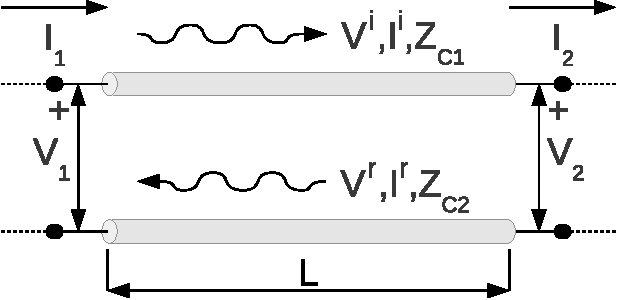
\includegraphics[width=0.5\columnwidth]{slike/sekcija.pdf}
\caption{Секција асиметричног вода дужине $L$}
\label{fpole}
\end{figure}

Циљ нам је да добијемо $ABCD$ параметре у функцији од параметара вода изведених у претходној секцији, наиме константе пропагације $\gamma$ (исте за оба правца простираања), дефинисане у (\ref{dispg}), и карактеристичних импеданси $Z_{c1}$ и $Z_{c2}$ (за инцидентни и рефлектовани талас, респективно), дефинисане у (\ref{zceta}). У сврху тога, представићемо стање на воду у било којој тачки помоћу напона инцидентног и рефлектованог таласа, $V^i$ и $V^r$, респективно. Релација између ових напона на портовима 1 и 2, у матричном облику, биће:
\begin{equation}\label{modal_basis}
\begin{bmatrix} V^i_1 \\ V^r_1 \end{bmatrix} =
\begin{bmatrix} e^{\gamma l} & 0 \\ 0 & e^{-\gamma l} \end{bmatrix}
\begin{bmatrix} V^i_2 \\ V^r_2 \end{bmatrix}.
\end{equation}
Укупни напон и струја у било којој тачки вода могу се представити као:
\begin{equation}\label{slicnost}
\begin{bmatrix} V \\ I \end{bmatrix} =
\begin{bmatrix} 1 & 1 \\ \frac{1}{Z_{c1}} & -\frac{1}{Z_{c2}} \end{bmatrix}
\begin{bmatrix} V^i \\ V^r \end{bmatrix} = 
Q\begin{bmatrix} V^i \\ V^r \end{bmatrix}.
\end{equation}
Инверзна релација је:
\begin{equation}\label{slicnost2}
\begin{bmatrix} V^i \\ V^r \end{bmatrix} =
Q^{-1}\begin{bmatrix} V \\ I \end{bmatrix}.
\end{equation}
%By substituing (\ref{slicnost2}) into (\ref{modal_basis}), we obtain:
%\begin{equation}
%Q^{-1}\begin{bmatrix} V_1 \\ I_1 \end{bmatrix} =
%\begin{bmatrix} e^{\gamma l} & 0 \\ 0 & e^{-\gamma l} \end{bmatrix}
%Q^{-1}\begin{`bmatrix} V_2 \\ I_2 \end{bmatrix}.
%\end{equation}
Заменом (\ref{slicnost2}) у (\ref{modal_basis}) и множењем са $Q$ са леве стране добијамо $ABCD$ матрицу:
\begin{equation}\label{decomp}
ABCD = Q\begin{bmatrix} e^{\gamma l} & 0 \\ 0 & e^{-\gamma l} \end{bmatrix}Q^{-1},
\end{equation}
која се, после замене вредности $Q$ и мало сређивања, своди на:
\begin{equation}\label{abcd}
\begin{bmatrix}
\cosh{\gamma l} + \dfrac{\eta}{Z_c}\sinh{\gamma l } & \left( Z_c - \dfrac{\eta^2}{Z_c} \right) \sinh{\gamma l} \\
\dfrac{\sinh{\gamma l}}{Z_c} & \cosh{\gamma l} - \dfrac{\eta}{Z_c}\sinh{\gamma l }
\end{bmatrix}.
\end{equation}
Може се видети из (\ref{abcd}) да када је $\eta = 0$, односно у симетричном случају, $ABCD$ се своде на случај вода са обичним диелектриком.

\subsection{Екстракција параметара}
Параметри расејања ($S$-параметри) се најчешће добијају као резултат мерења или ЕМ симулације, и могу се једнозначно трансформисати у $ABCD$ матрицу~\cite{Pozar:05}. Када је добијемо, лако се види из (\ref{abcd}) да се ефективни параметри могу добити на следећи начин:
\begin{align}
\gamma & = \pm \cosh^{-1}\frac{A+D}{2},\label{a2gama}\\
Z_c & = \frac{\sinh{\gamma l}}{C} = \pm\frac{1}{C}\sqrt{1 - \left( \frac{A+D}{2}\right)^2},\label{a2zc}\\
\eta & = \frac{A-D}{2C}.\label{a2eta}
\end{align}
%Уколико је јединична ћелија симетрична\footnote{Симетрија имплицира $A=D$ за $ABCD$ параметре, и $S_{11}=S_{22}$ за $S$-параметре.}, можемо заменити $S$-параметре и поједноставити изразе тако да се добије
%\begin{eqnarray}
%\gamma = \pm\frac{1}{L}\cosh^{-1}\frac{1-S_{11}^2+S_{21}^2}{2S_{21}},\label{s2gama} \\
%Z_c = \pm \sqrt{\frac{(1+S_{11})^2-S_{21}^2}{(1-S_{11})^2-S_{21}^2}}\label{s2zc},
%\end{eqnarray}
%и $\eta = 0$, што се слаже са претходним резултатима за НРВ процедуру, што је било очекивано~\cite{Smith:02, Mao:05, Chen:04}. %ovaj pasus treba dide dole

Неколико додатних коментара је потребно у вези датих релација. Најпре, знак у (\ref{a2gama}) треба изабрати у складу са критеријумом пасивности, 
\begin{equation}\label{pasivnost}
\mathrm{Re}\left\lbrace\gamma\right\rbrace > 0.
\end{equation}
Ипак, остаје проблем гранања функције $\cosh^{-1}{z}$, који доводи до неодређености у имагинарном делу $\gamma$ (односно, у реалном делу $n$). Ово је последица чињенице да је немогуће разликовати промену фазе од $\phi$ до $\phi + 2k\pi, k\in Z$. Један приступ за решавање овог проблема је коришћење Крамерс-Кронигових релација да се процени тачна грана~\cite{Szabo:10}.

У већини претходних извештаја~\cite{Nicol:70, Weir:74, Smith:02, Markos:03, Mao:05}, знак карактеристичне импедансе у (\ref{a2zc}) или (\ref{s2zc}) се бира на основу критеријума $\mathrm{Re}\{Z_c\}>0$ или сличног, који може бити веома осетљив на мале нумеричке грешке~\cite{Chen:04}. Ипак, јасно се види из (\ref{a2zc}) да је знак каркатеристичне импедансе повезан са знаком константе простирања у (\ref{a2gama}), дакле, само један критеријум је довољан, као што је показано у~\cite{Chen:04}.

\subsection{Ефективни параметри еквивалентног медијума}
Када је одређена константа простирања, $\gamma$, и карактеристична импеданса еквивалентног вода, $Z_{c1,2}$, индекс преламања, $n$, и карактеристична импеданса еквивалентног медијума, $z_{1,2}$, се лако добијају
\begin{equation}\label{nz}
n = -j\frac{c}{\omega}\gamma,\quad z_{1,2}=\frac{Z_{c1,2}}{Z_{вазд.}}.
\end{equation}
Ефективни параметри бианизотропног медијума, $\varepsilon$, $\mu$ и $u$ могу се изразити преко $n$ и $z_{1,2}$ преуређењем (\ref{dispn}) и (\ref{dispz}):
\begin{equation}\label{effp}
\begin{split}
	\varepsilon = \frac{2n}{z_1+z_2},\quad
	\mu = 2n\frac{z_1z_2}{z_1+z_2},\quad
	u = -jn\frac{z_1-z_2}{z_1+z_2}.
\end{split}
\end{equation}
Комбинација (\ref{nz}) и (\ref{effp}) са изразима који их повезују са $S$-параметрима изведеним раније омогућава ектстракцију ефективних параметара из симулираних или експерименталних података. Ове релације ћемо надаље обележавати као генералисани поступак ($ГП$).

Још једна могућност за опис асиметричних јединичних ћелија је коришћење $\varepsilon$ и $\mu$ који зависе од смера простирања таласа. Они се могу добити као
\begin{equation}
\varepsilon_{1,2}=\frac{n}{z_{1,2}};\quad \mu_{1,2}=nz_{1,2}.
\end{equation}
Иако је математички еквиваленан претходном, овај приступ нема директну физичку интерпретацију. Међутим, показаће се као изузетно користан за валидацију ефективних параметара у секцији~\ref{sekc4}, због чега ће бити укључен у примере екстракције, где ће се реферисати као генералисани поступак за инцидентни талас на порту 1 и порту 2 ($ГП_1$ и $ГП_2$, респективно).

\subsection{Николсон-Рос-Вир процедура са усредњавањем}

Као што је речено у уводу, за екстракцију параметара се најчешће користи тзв. Николсон-Рос-Вир (\foreign{Nicolson-Ross-Weir}, НРВ) процедура, која претпоставља да је испитивани узорак симетричан, односно да важи $S_{11}=S_{22}$~\cite{Nicol:70, Weir:74, Smith:02}. Како би се заобишло ово ограничење у случају асиметричних узорака, предложено је коришћење геометријске средине рефлексије, $S_{11ср}=\sqrt{S_{11}S_{22}}$~\cite{smith:05}; овај поступак ће бити означаван као $НРВ_{ср}$. Како би се јасније представиле сличности и разлике између $НРВ_{ср}$ и овде излаганог метода, изрази (\ref{a2gama})--(\ref{a2zc}) ће бити приказани преко $Ѕ$-параметара:
\begin{equation}\label{phy_gama}
\gamma=\mp\frac{1}{L}\cosh^{-1}{\frac{1-S_{11}S_{22}+S_{12}^2}{2S_{12}}},%=\mp\frac{jc}{\omega l}\cosh{\frac{1-S_{11avg}^2+S_{12}^2}{2S_{12}}},
\end{equation}
\begin{equation}\label{phy_zc}
Z_{c} = \frac{2S_{12}\sqrt{1-\left( \frac{1-S_{11}S_{22}+S_{12}^2}{2S_{12}} \right)^2}}{1-S_{11}-S_{22}+S_{11}S_{22}-S_{12}^2}. (избачено Z_0?)
\end{equation}
Уколико је ћелија симетрична, $Ѕ_{11}=Ѕ_{22}$, горњи изрази ће се поједноставити у
\begin{eqnarray}
\gamma = \pm\frac{1}{L}\cosh^{-1}\frac{1-S_{11}^2+S_{21}^2}{2S_{21}},\label{s2gama} \\
Z_c = \pm \sqrt{\frac{(1+S_{11})^2-S_{21}^2}{(1-S_{11})^2-S_{21}^2}}\label{s2zc}.
\end{eqnarray}
Суштински, $НРВ_{ср}$ процедура се базира на замени $Ѕ_{11}$ у изразима (\ref{s2gama})--(\ref{s2zc}) са $\sqrt{Ѕ_{11}Ѕ_{22}}$. Лако се види да ће израз за константу простирања (\ref{s2gama}) приликом ове замене претворити у тачан израз (\ref{phy_gama}). С друге стране, израз за импедансу (\ref{s2zc}) неће бити еквивалентан изразу (\ref{phy_zc}), услед постојања линеарних чланова у имениоцу. Због тога ће се карактеристичне импедансе добијене помоћу два метода разликовати; при томе у случају $НРВ_{ср}$ израз није добијен полазећи од почетних дефиниција, као код ГП метода, већ донекле арбитрарним поступком усредњавања. Такође, пошто импеданса фигурише у изразима ефективних $\varepsilon$ и $\mu$, разлике ће се пренети и на њих. У наставку ће бити дато поређење екстрахованих ефективних параметара на оба начина за различите практичне случајеве, где ће бити показана већа утемељеност ГП метода у случајевима са израженом асиметријом.

\section{Асиметричне јединичне ћелије}\label{sekc3}

У овом делу се врши испитивање електромагнетних својстава метаматеријала на бази водова, који се састоји од микрострип вода спрегнутог са (бродсајд-каплд??) сплит-ринг резонаторима, постављеним са једне стране вода.

Показано је да се ротирањем појединачних сплит-рингова значајно утиче на електромагнетне особине [метаматеријала на бази водова], због другачијих електричних и магнетних интеракција услед другачије међусобне оријентације сплит-рингова у простору и због другачије оријентације у односу на вод (грозна реченица!!)~\cite{stereo,bib9}.

Коришћењем предложеног генералисаног поступка екстракције, истраживаће се нове асиметричне јединичне ћелије реализоване на двослојном супстрату. Ивице прстенова које садрже процепе постављене су једна изнад друге, а не на супротним странама као што је то уобичајено [код БСЦ СРР-ова]. За разлику од уобичајеног дизајна, нови СРР-ови имају резонантне учестаности међусобно много ближе (око 500\,MHz), што је погодно за савремене бежичне системе.

Испитиваће се два типа СРР-ова: са процепима паралелним и нормалним у односу на вод. Процепи могу да се померају симетрично лево и десно у односу на центар ивице на којој се налазе, као што је приказано на сл.~\ref{fig4} за СРР-ове са паралелним процепима.

Како би се испитала ефективност предложене методе у односу на $НРВ_{ср}$ поступак, тестиране су структуре које имају слабо изражену асиметрију, код којих је процеп паралелан воду, као и оне које су наглашено асиметричне, код којих је процеп нормалан на вод.

\subsection{Јединичне ћелије са паралелним процепом [у односу на вод]}

Овај тип јединичних ћелија може имати процепе на ивицама које су ближе воду или даље од њега, као што је приказано на сл.~\ref{fig4}. Јединичне ћелије састоје се од [broadside coupled] СРР-ова са процепима симетрично помереним од центра. Асиметрија је узрокована само чињеницом да су процепи у различитим слојевима супстрата (горњем и доњем). Микрострип вод је повезан са масом (проводном равни) преко цилиндричне вије, пречника $R_v$, постављеном у центру ћелије између референтних равни (означених испрекиданим линијама).

Јединичне ћелије су симулиране помоћу програма WIPL-D Pro 10.0, намењеног за 3Д електромагнетну анализу~\cite{wipl}, који је базиран на методи момената; $S$-параметри су деембедовани на референтним равнима. Биће упоређена екстракција бианизотропних параметара, $ГП$, асиметрична екстракција која даје два скупа параметара, $ГП_{1,2}$ као и стандардни поступак са усредњавањем $НРВ_{ср}$.
\begin{figure}[!t]
\subfloat[]{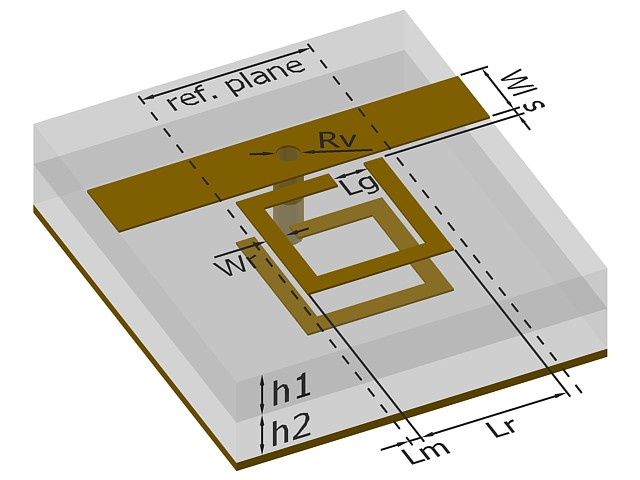
\includegraphics[width=0.45\textwidth]{slike/p1.jpeg}
\label{fig4a}}\hfill
\subfloat[]{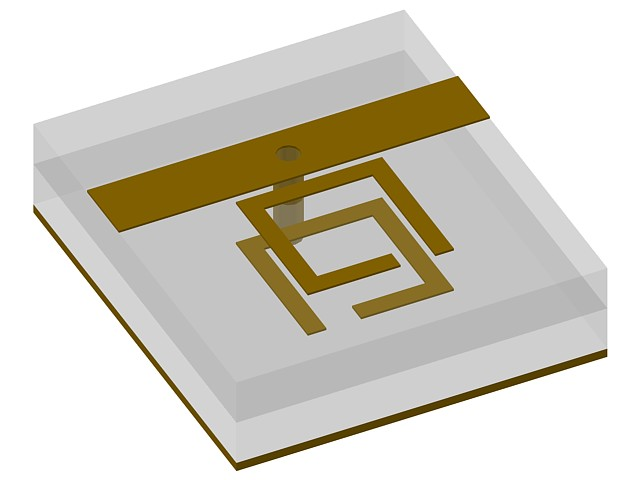
\includegraphics[width=0.45\textwidth]{slike/p2.jpeg}
\label{fig4b}}
\caption{Јединичне ћелије са процепима помереним на супротне стране у односу на средину ивице прстена: (а) процепи близу вода, (б) процепи даље од вода. Релевантне димензије: $h_1~=~0.635\,\mathrm{mm}$, $h_2=1.575\,\mathrm{mm}$, $\varepsilon_{r1}=10.2$, $\varepsilon_{r2}=2.2$, $L_r=3.15\,\mathrm{mm}$, $L_g=0.75\,\mathrm{mm}$, $L_a=2\,\mathrm{mm}$, $L_m=0.25\mathrm{mm}$, $L= L_r +2L_m$, $W_l=1.4\,\mathrm{mm}$, $W_r=0.4\,\mathrm{mm}$, $R_v=0.5\,\mathrm{mm}$, $s=0.2\,\mathrm{mm}$.}
\label{fig4}
\end{figure}

Магнитуда $S$-параметара за јединичне ћелије са процепима близу вода [сл.~\ref{fig4a}] приказана је на сл.~\ref{fig5a}. Може се видети да разлика између коефицијената рефлексије $S_{11}$ и $S_{22}$ постоји само у околини прве резонансе. Екстраховани индекс преламања на сл.~\ref{fig5b} је исти код свих поступака, захваљујући погодно дефинисаној средњој вредности код $НРВ_{ср}$. Јединична ћелија испољава ,,леворуки`` опсег око \SI{5.5}{\giga\hertz}, осенчен на графику, и ,,десноруки`` опсег око \SI{6.15}{\giga\hertz}, који одговара другој резонанси.
\begin{figure}[!t]
\subfloat[]{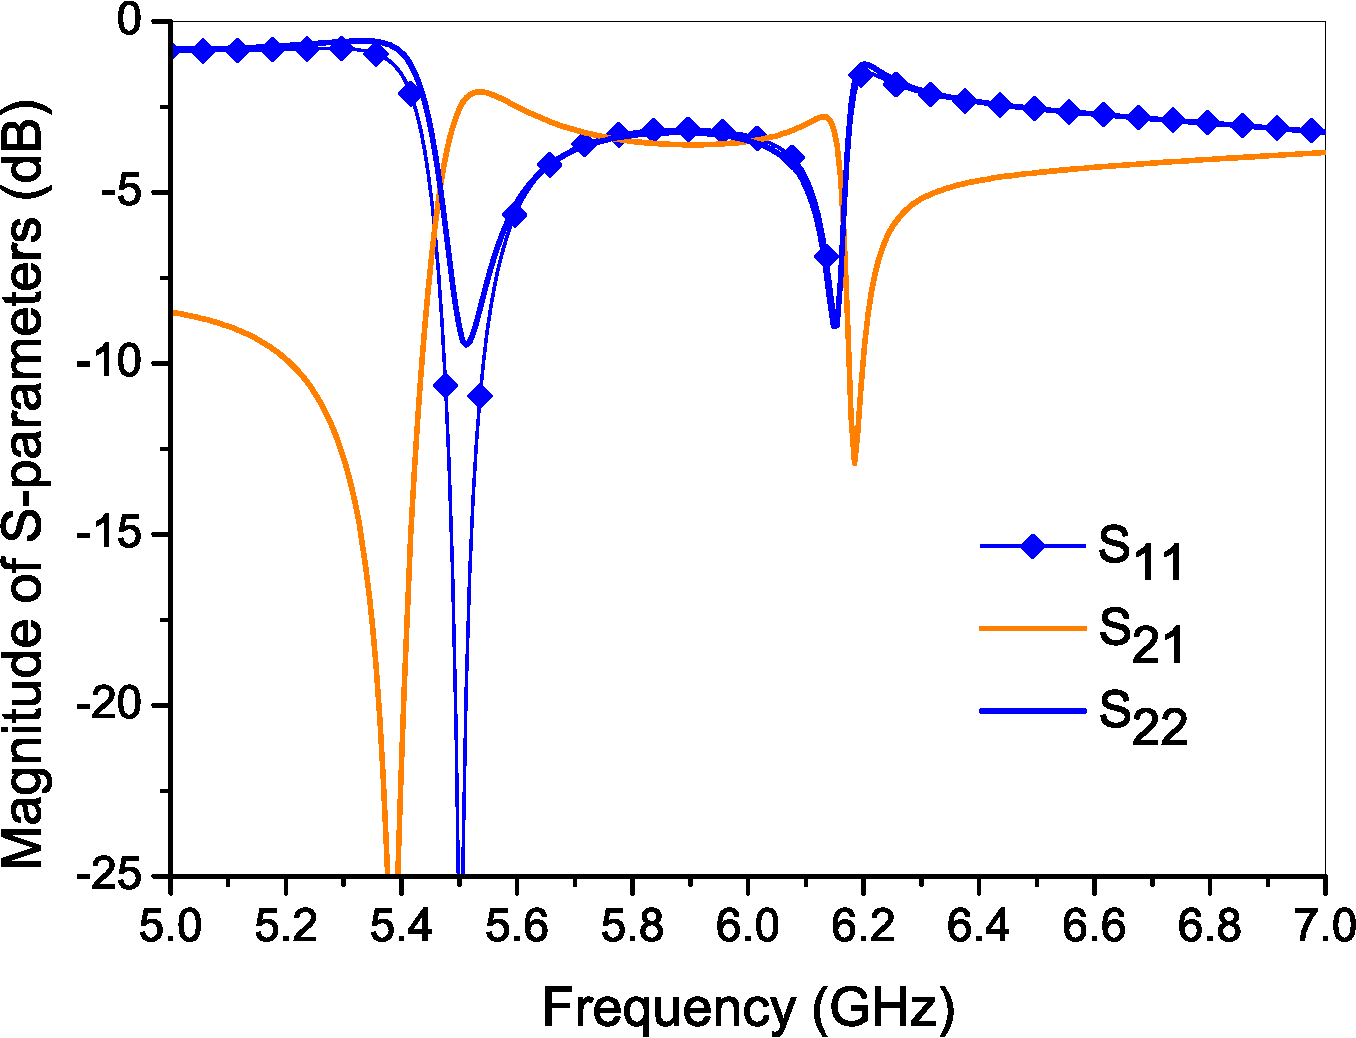
\includegraphics[scale=\SkalaA]{slike/5a.pdf}
\label{fig5a}}\hfill
\subfloat[]{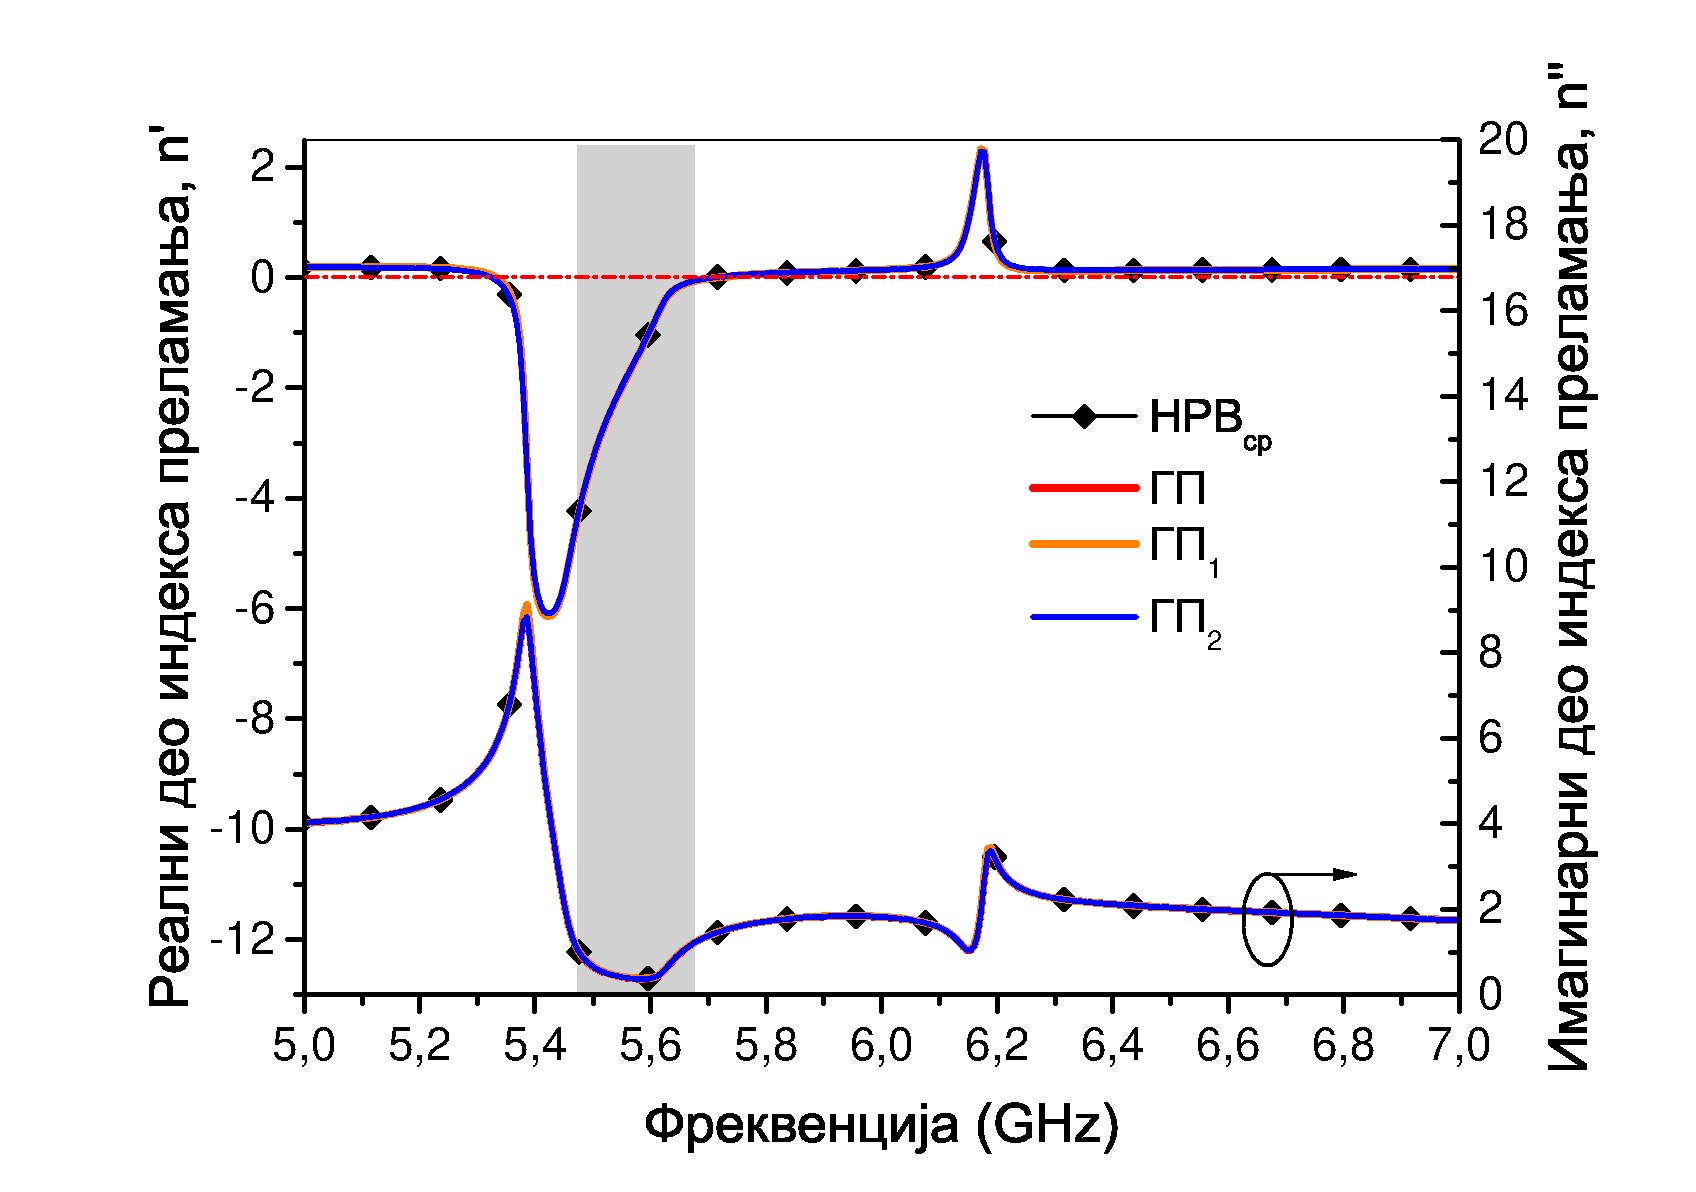
\includegraphics[scale=\SkalaA]{slike/5b.pdf}
\label{fig5b}}
\caption{Јединичне ћелије са АСРР-овима са процепом близу вода: (а) магнитуда $S$-параметара, (б) екстраховани индекс преламања. Осенчени правоугаоник означава фреквенцијски опсег са двоструко негативним параметрима.}
\label{fig5}асдф
\end{figure}адсф 

Карактеристичне импедансе, екстраховане помоћу различитих метода, су упоређене на сл.~\ref{fig7}. Може се видети да се вредности добијене помоћу $ГП$ налазе тачно између вредности добијених преко $ГП_{1,2}$, као што је очекивано на основу релације (12). Важно је истаћи да је само на првој резонанси вредност добијена $НРВ_{ср}$ методом другачија, али незнатно, од вредности добијене $ГП$ методом, што значи да асиметрија није знатно изражена.
\begin{figure}[!t]
\centering
\includegraphics[scale=\SkalaB]{slike/11a.pdf}
\caption{Карактеристична импеданса екстрахована различитим поступцима за јединичне ћелије са АСРР-овима са процепом близу вода.}
\label{fig7}
\end{figure} 

\subsection{Јединичне ћелије са процепима далеко од вода}

Јединичне ћелије са процепима даље од вода, сл.~\ref{fig4b}, имају доста другачије $Ѕ$-параметре и екстраховани индекс преламања од ћелија са процепом близу вода [видети сл.~\ref{fig8} и сл.~\ref{fig8b}]. Разлика између коефицијената рефлексије на портовима 1 и 2 се јавља код друге резонансе, што је евидентно у њиховој фази на сл.~\ref{fig8c}. Екстраховани индекс преламања, приказан на сл.~\ref{fig8b}, има два ,,леворука`` опсега око 5.9\,GHz и 6.35\,GHz, који су означени осенченим правоугаоницима.
\begin{figure}[!t]
\subfloat[]{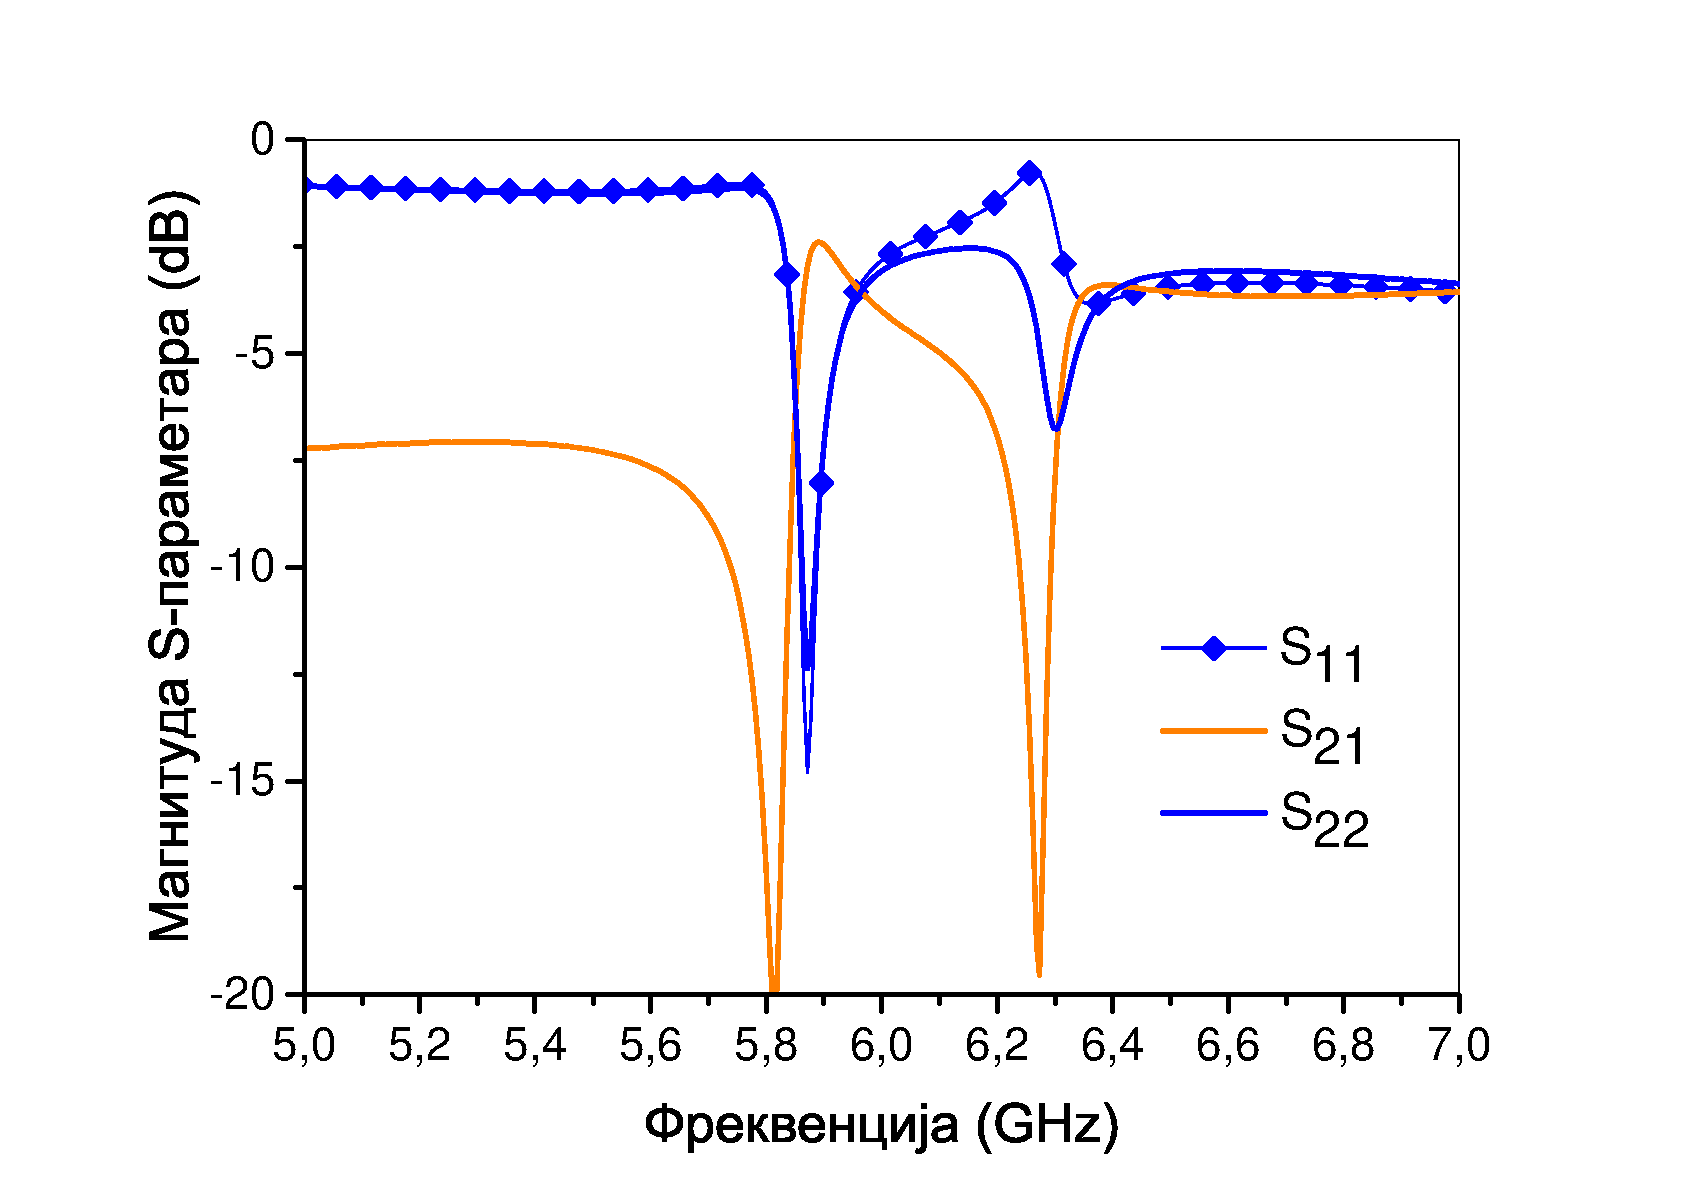
\includegraphics[scale=\SkalaA]{slike/8a.pdf}
\label{fig8a}}\hfill
\subfloat[]{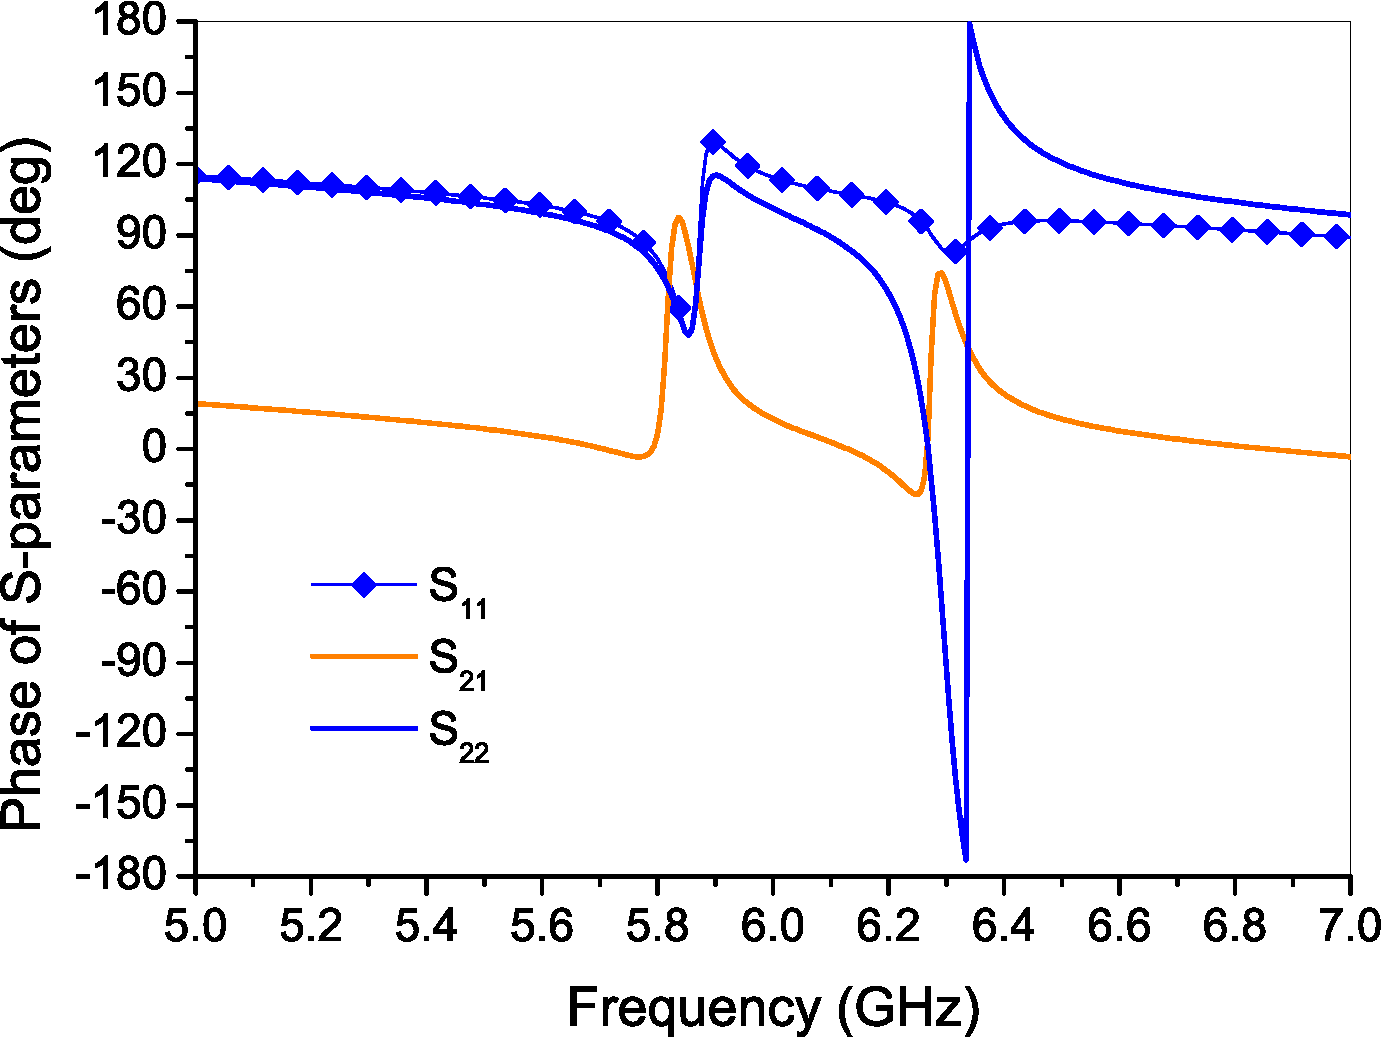
\includegraphics[scale=\SkalaA]{slike/8c.pdf}
\label{fig8c}}
\caption{Магнитуда (а) и фаза (б) $S$-параметара за АСРР-ове са процепима даље од вода.}
\label{fig8}
\end{figure}
\begin{figure}[!t]
\centering
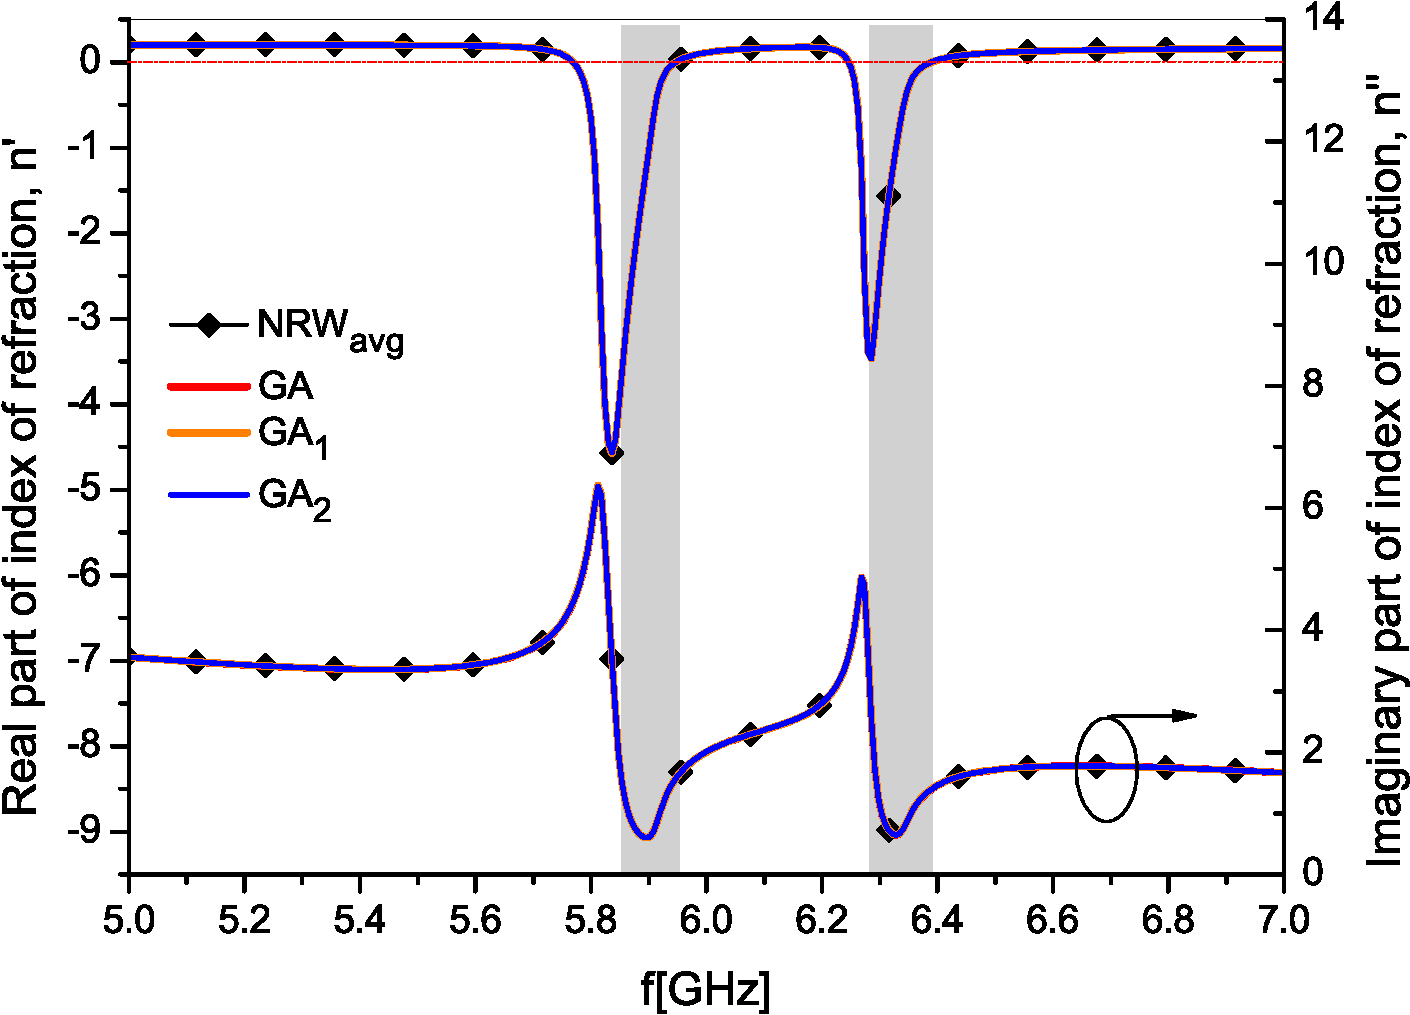
\includegraphics[scale=\SkalaB]{slike/8b.pdf}
\caption{Ефективни индекс преламања, екстрахован различитим поступцима, за јединичне ћелије са АСРР-овима са процепом даље од вода. Осенчени правоугаоници означавају фреквенцијске опсеге са двоструко негативним параметрима.}
\label{fig8b}
\end{figure} 
\begin{figure}[!t]
\subfloat[]{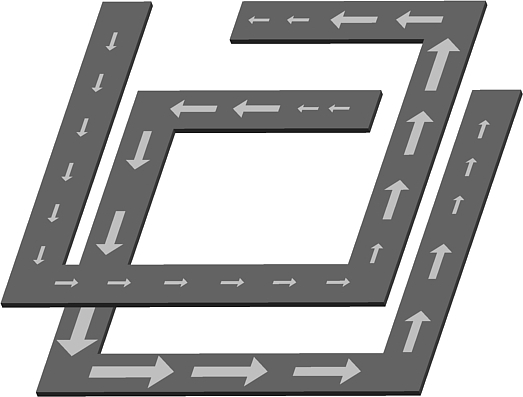
\includegraphics[width=0.45\textwidth]{slike/9a.jpeg}
\label{fig9a}}\hfill
\subfloat[]{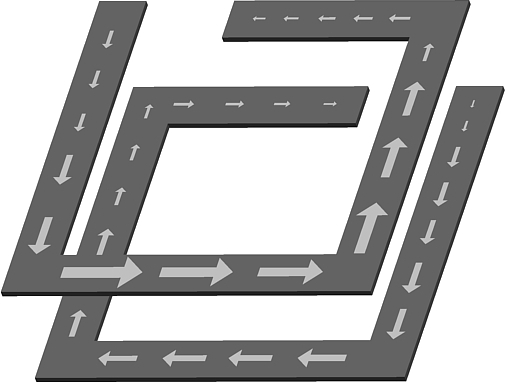
\includegraphics[width=0.45\textwidth]{slike/9b.jpeg}
\label{fig9b}}
\caption{Расподела струја, да ли то да убацим? Local induced current distribution at resonant frequencies: (а)~symmetric mode at $f=\SI{5.9}{\giga\hertz}$ and (б) anti-symmetric mode at $f=\SI{6.35}{\giga\hertz}$. Length of the arrows are proportional to the intensity of the current.}
\label{fig9}
\end{figure}

Екстрахована ефективна пермитивност, пермеабилност и карактеристична импеданса, коришћењем $ГП$, $ГП_{1,2}$ и $НРВ_{ср}$ приказани су на сл.~\ref{fig10}. Са слике се види да све методе дају исте резултате у опсегу где је одзив симетричан ($S_{11} = S_{22}$). Ефективни параметри добијени помоћу ГП и $НРВ_{ср}$ се разликују само око друге резонансе, где је асиметрија најизраженија, што је обележено осенченим правоугаоницима на сл.~\ref{fig10}. У целом опсегу учестаности од интереса ефективна пермитивност добијена $НРВ_{ср}$ и ГП методама је негативна, док ефективна пермеабилност мења знак на две резонансе које одговарају ,,леворуким`` опсезима.
\begin{figure}[!t]
\centering
\subfloat[]{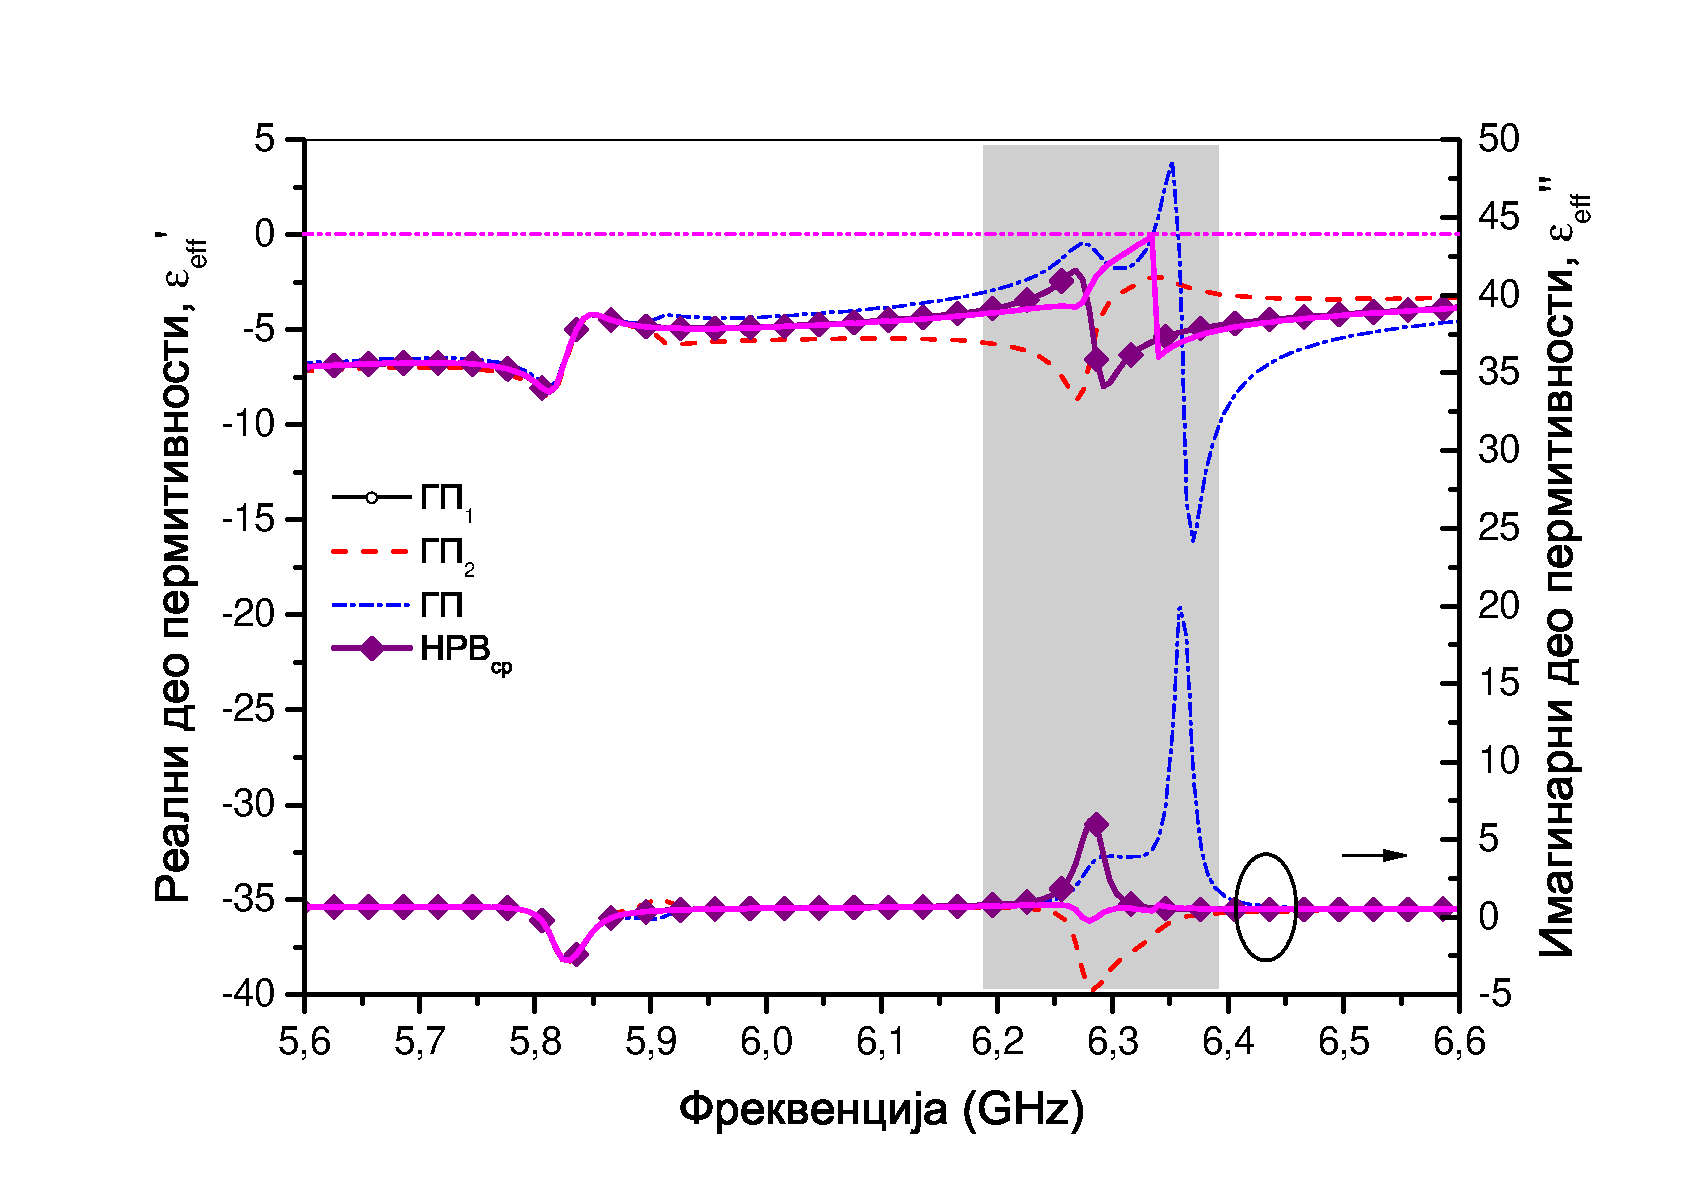
\includegraphics[width=0.6\textwidth]{slike/10a.pdf}
\label{fig10a}}\hfill
\subfloat[]{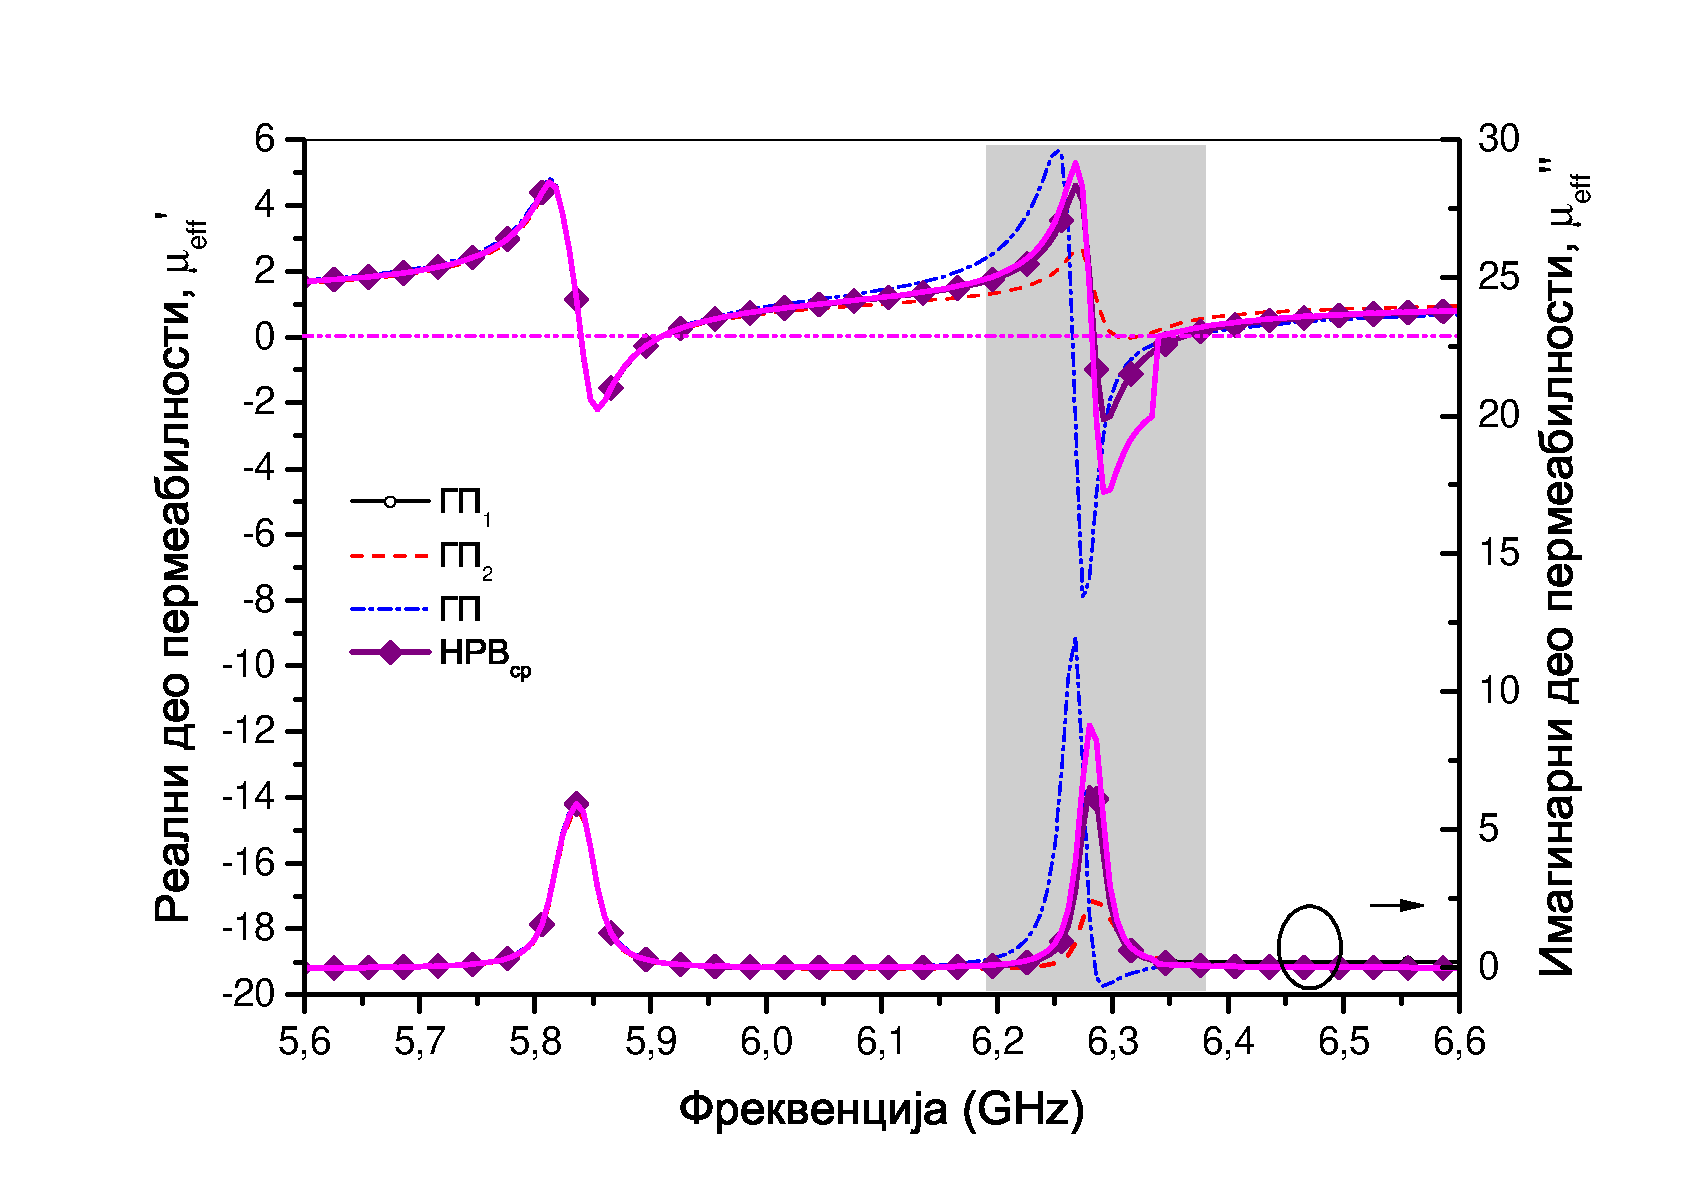
\includegraphics[width=0.6\textwidth]{slike/10b.pdf}
\label{fig10b}}\\
\subfloat[]{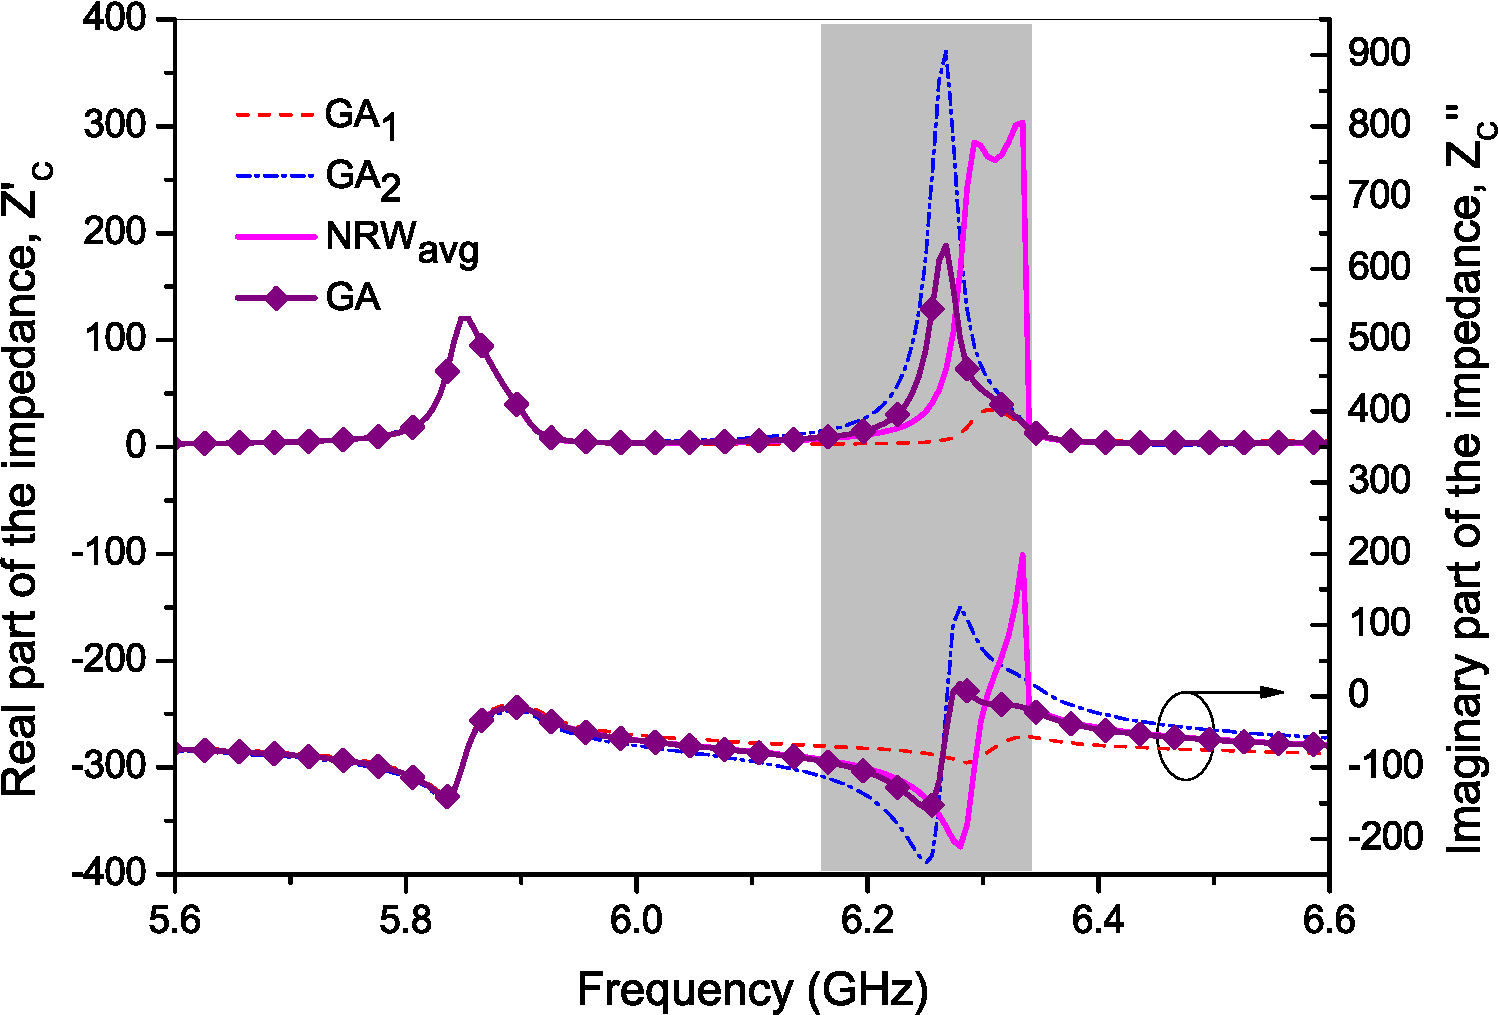
\includegraphics[width=0.6\textwidth]{slike/11b.pdf}
\label{fig11b}}
\caption{Ефективна пермитивност (а), пермеабилност (б) и карактеристична импеданса (в) екстрахована за АСРР-ове са процепима даље од вода. Осенчени правоугаоници означавају опсеге где $НРВ_{ср}$ и ГП дају различите резултате.}
\label{fig10}
\end{figure} 

%In Fig.~\ref{fig11} we compare characteristic impedances extracted using different retrieval procedures for unit cells with ASRRs. It can be seen that the different retrieval procedures give very different results at the first and second resonances for the case with gaps near and far from ML respectively. Difference is particularly pronounced if the gaps are far from ML as it is indicated by rectangular bar in Fig.~\ref{fig11b}. 
%\begin{figure}[!t]
%\subfloat[]{\includegraphics[width=\sirina]{slike/11a}
%\label{fig11a}}
%\subfloat[]{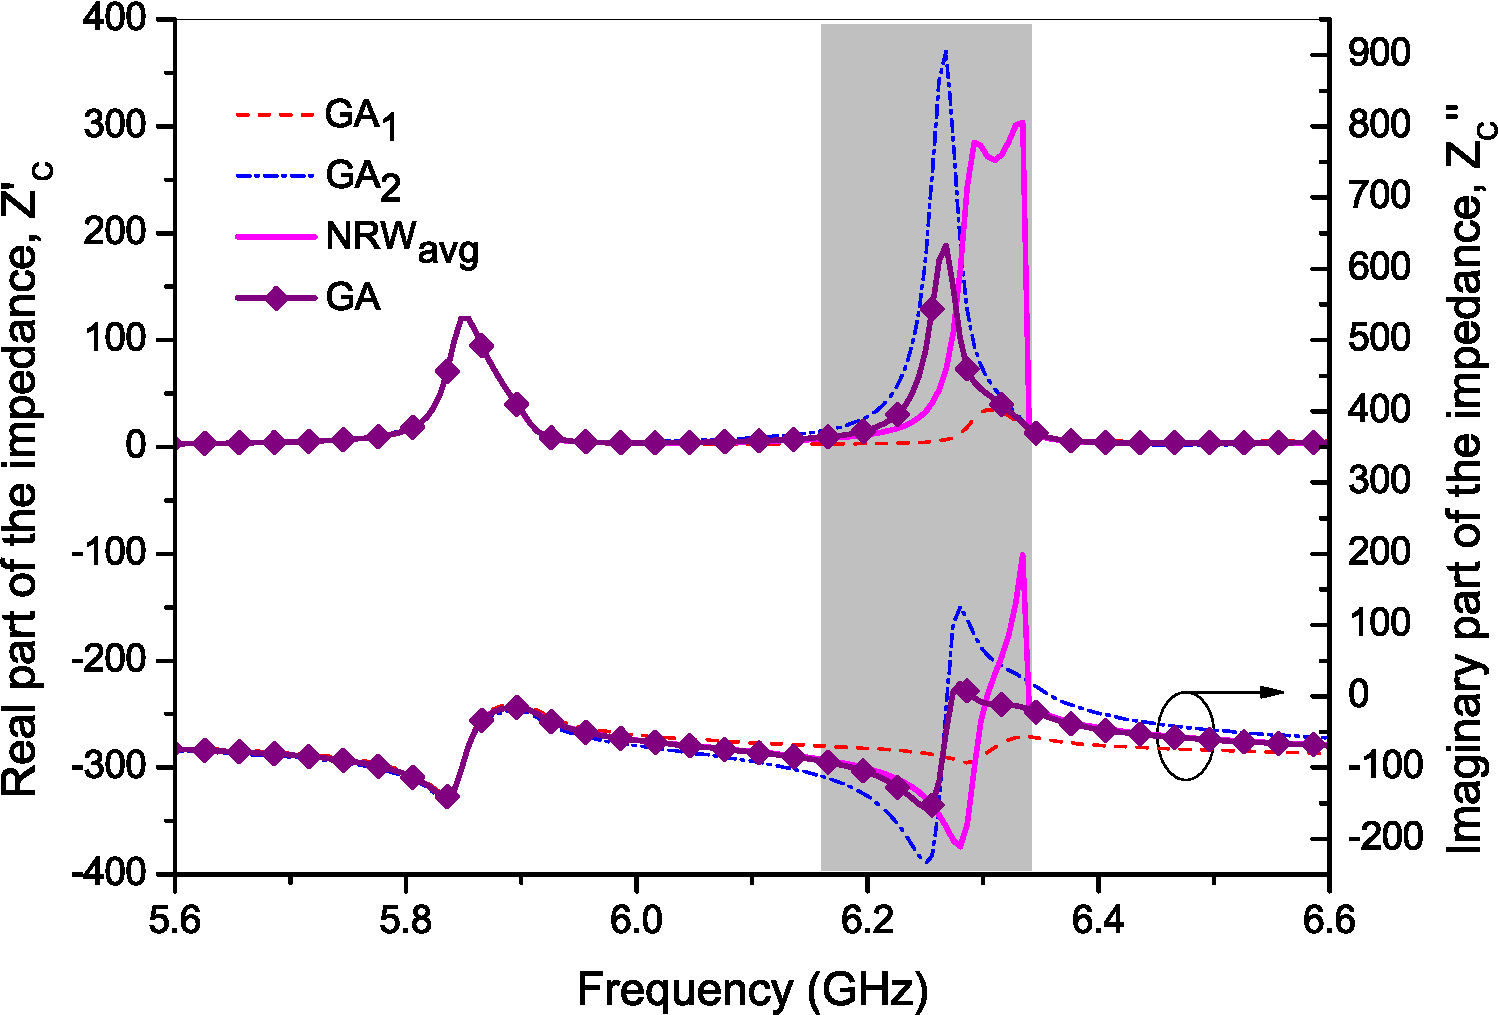
\includegraphics[width=\sirina]{slike/11b}
%\label{fig11b}}
%\caption{The effective characteristic impedance extracted using different retrieval procedures for unit cells with ASRRs: (a) with gaps near ML and (b) with gaps far from ML. Rectangular bars denote frequency range in which NRWavg and GA give different results.}
%\label{fig11}
%\end{figure} 

Генералисани поступак екстракције уводи два нова параметра, као меру асиметрије јединичне ћелије: $u$ и $\eta$. Сл.~\ref{fig12} јасно показује да јединичне ћелије са процепима даље од вода имају максималне вредности $u$ и $\eta$ параметара око три пута веће него ћелије са процепима ближе воду. Такође се види да се бианизотропија јавља у близини или прве или друге резонансе одговарајућих ћелија. Интересантно је напоменути да је бианизотропија драстично мања уколико су процепи постављени на супротним странама СРР-ова, као код стандардних БСЦ?? СРР-ова, чак и када су процепи померени од центра ивице. У том случају бианизотропија се јавља на обе резонансе.
%\begin{figure}[!t]
%\centering
%\includegraphics[scale=\SkalaB]{slike/graf_cr/11a}
%\caption{The extracted characteristic impedance extracted using different retrieval procedures for unit cell with ASRRs with gaps near ML.}
%\label{fig7}
%\end{figure} 
\begin{figure}[!t]
\centering
\subfloat[]{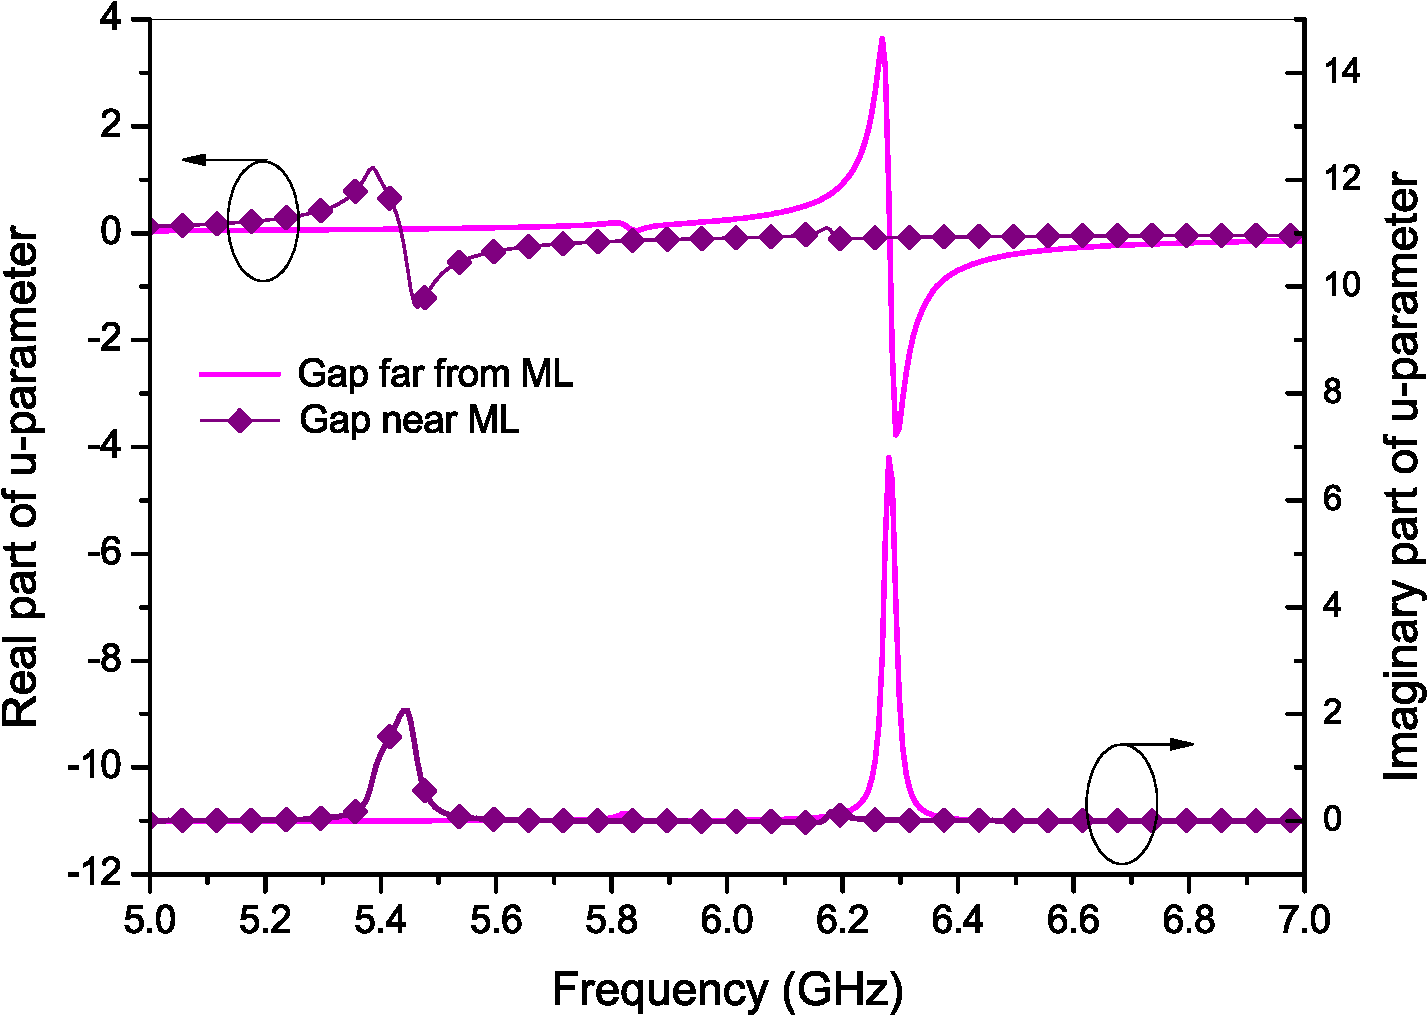
\includegraphics[width=0.6\textwidth]{slike/12a.pdf}
\label{fig12a}}\hfill
\subfloat[]{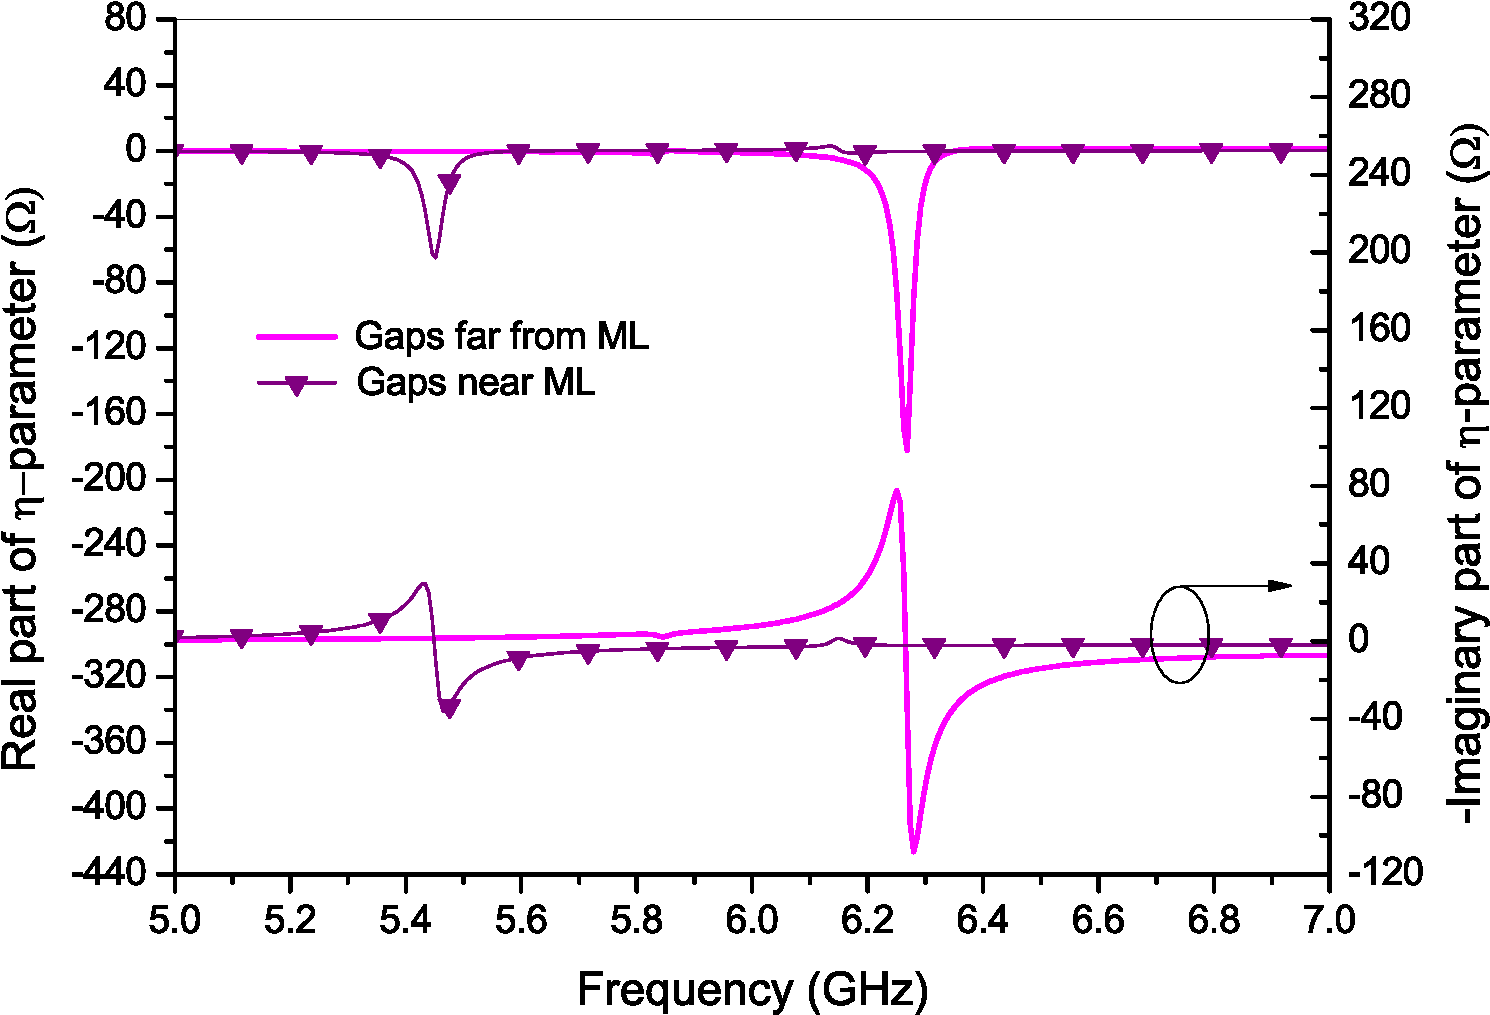
\includegraphics[width=0.6\textwidth]{slike/12b.pdf}
\label{fig12b}}
\caption{Поређење екстрахованих параметара: (а) параметар бианизотропије $u$ и (б) разлика ефективних карактеристичних импеданси, $\eta$, за ћелије са процепом паралелним воду.}
\label{fig12}
\end{figure} 

На сл.~\ref{usl_par} упоређени су стандардни услов за негативни индекс преламања (\ref{usl_std}), који је валидан за симетричне ћелије, и последично за параметре добијене $НРВ_{ср}$ методом, и нови услов (\ref{usln}), који је изведен за асиметричне ћелије. Оба услова су израчуната помоћу параметара добијених ГП методом. У случају ћелија са паралелним процепом даље од вода, види се да су око прве резонансе обе криве преклопљене, јер је одзив симетричан у том опсегу. Око друге резонансе крива која одговара новом услову пресеца $x$-осу тачно на тачкама где је реални део индекса једнак нули, што није случај за криву која одговара стандардном критеријуму. У овом случају, стандардни критеријум предвиђа нешто шири опсег негативног индекса. На крају, применили смо стандардни услов на параметре добијене $НРВ_{ср}$ методом, и показује се да се добијена крива у потпуности преклапа са новим условом. Ово потврђује валидност новог услова, пошто оба метода дају исти индекс преламања, како у симетричном тако и у асиметричном случају.
\begin{figure}[!t]
\centering
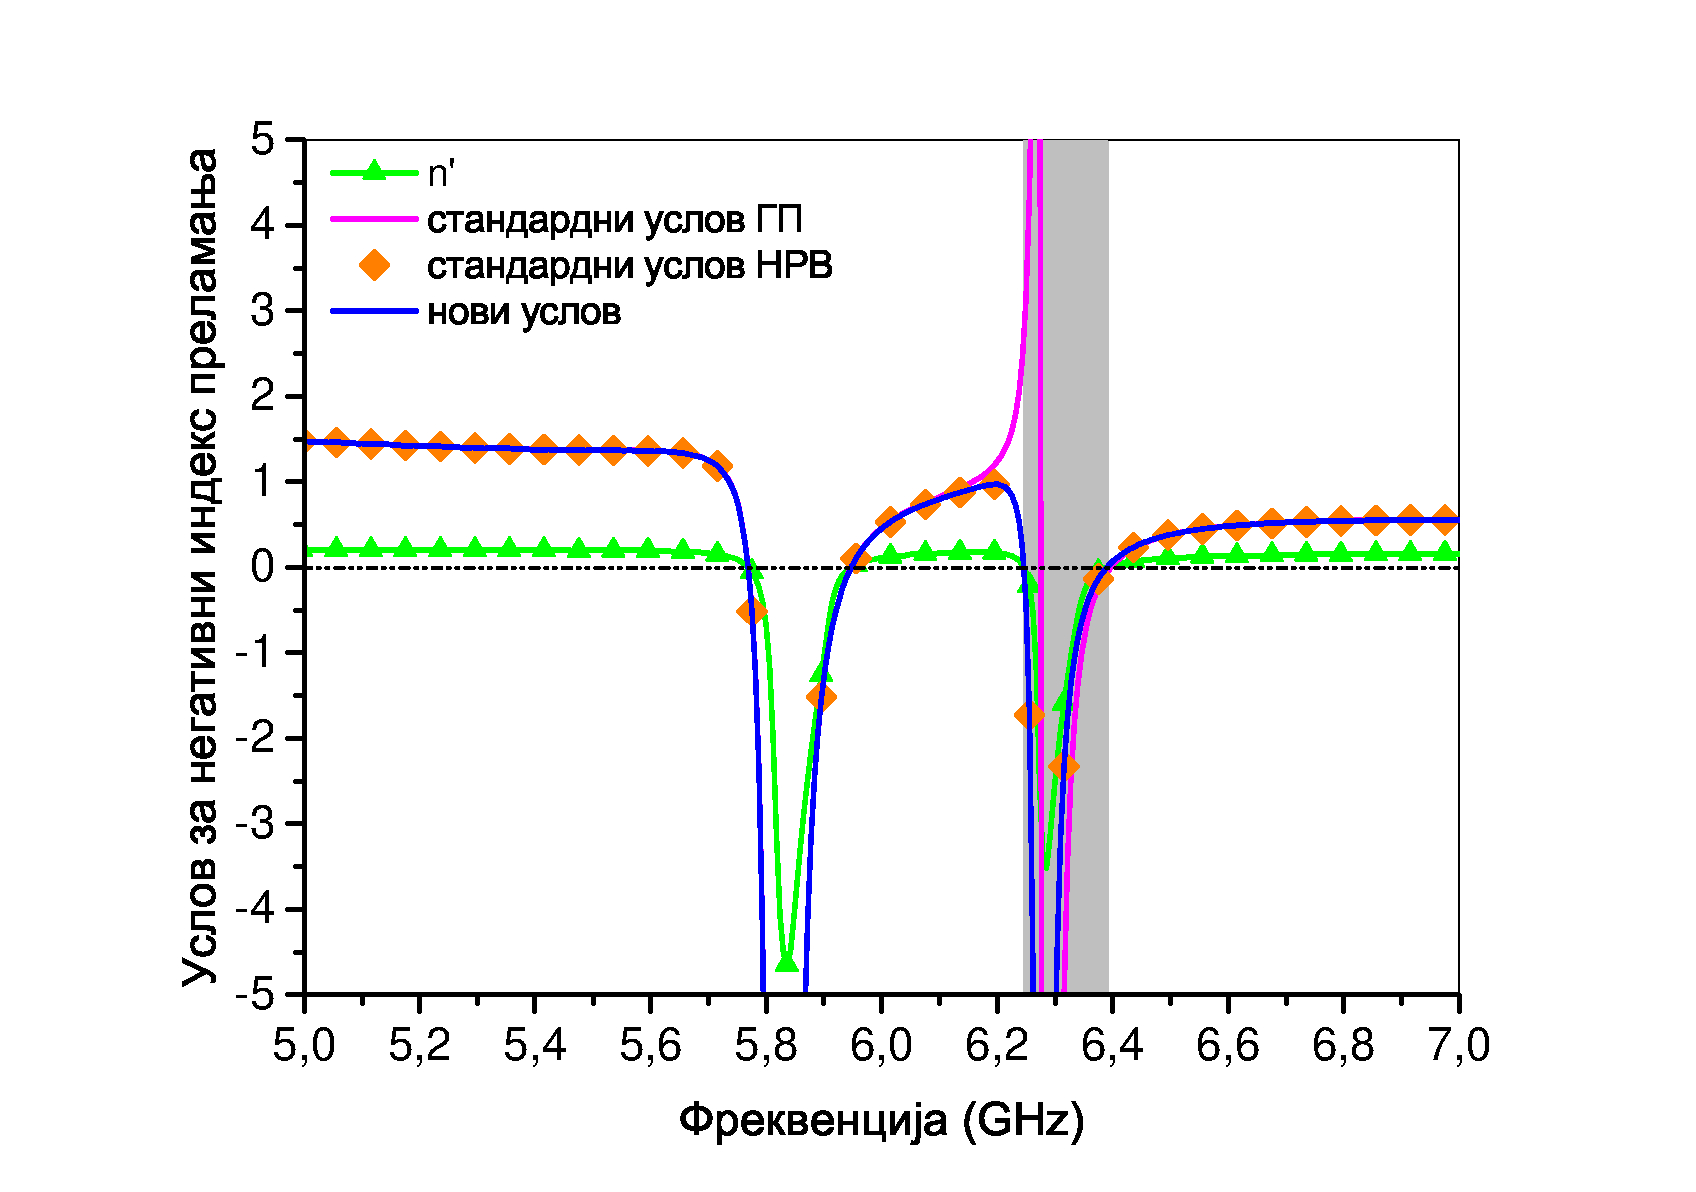
\includegraphics[width=0.6\textwidth]{slike/usl_par.pdf}
\caption{Поређење стандардног и новог критеријума за негативни индекс преламања за јединичну ћелију са процепима паралелним воду. Ефективни параметри су добијени ГП методом. Осенчени правоугаоник означава опсег у коме ћелија има асиметрични одзив и два критеријума предвиђају другачије опсеге негативног индекса.}
\label{usl_par}
\end{figure} 
	
\subsection{Јединичне ћелије са процепима нормалним на вод}

Јединичне ћелије са процепима нормалним у односу на микрострип вод су приказане на сл.~\ref{norm_gep}, и можемо разликовати два случаја у зависности од положаја горњег процепа: а) када је ближе воду и б) даље од њега. У оба случаја процепи су ближе порту 1 јединичне ћелије. Уколико бисмо заменили редослед портова, параметри $u$ и $\eta$ би променили знак, док би све остало било непромењено.
\begin{figure}[!t]
\subfloat[]{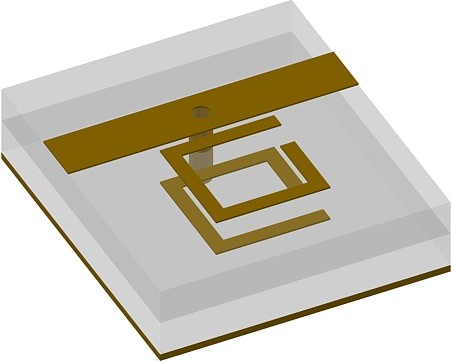
\includegraphics[width=0.45\textwidth]{slike/n1.jpeg}
\label{norm1}}\hfill
\subfloat[]{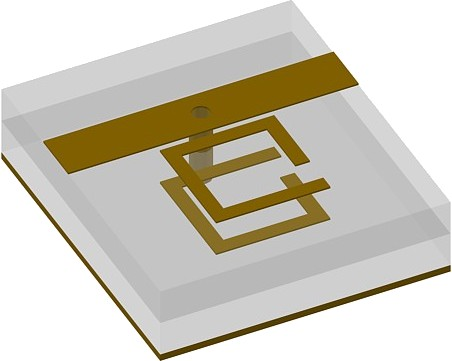
\includegraphics[width=0.45\textwidth]{slike/n2.jpeg}
\label{norm2}}
\caption{Изглед јединичних ћелија које се састоје од АСРР-ова са ивицом која садржи процеп нормалном на вод: (а) горњи процеп ближе воду, (б) горњи процеп даље од вода.}
\label{norm_gep}
\end{figure}

Магнитуда $Ѕ$-параметара за јединичне ћелије са нормалним процепом су приказане на сл.~\ref{fig14_1}. Екстрахована ефективна пермитивност и пермеабилност за случај са горњим процепом ближе и даље од вода су приказане на сл.~\ref{fig14_2}-\ref{fig14_3}, респективно. Може се видети да положај нормалних процепа не утиче на резонантне учестаности у значајној мери. Такође $S_{11}$ се разликује од $S_{22}$ на обе резонансе, али наглашеније на првој. Екстрахована пермитивност и пермеабилност коришћењем ГП и $НРВ_{ср}$ метода се значајно разликују око 5.7\,GHz, не само по апсолутној вредности, већ имају и супротне знакове.
\begin{figure}[!t]
\centering
\subfloat[]{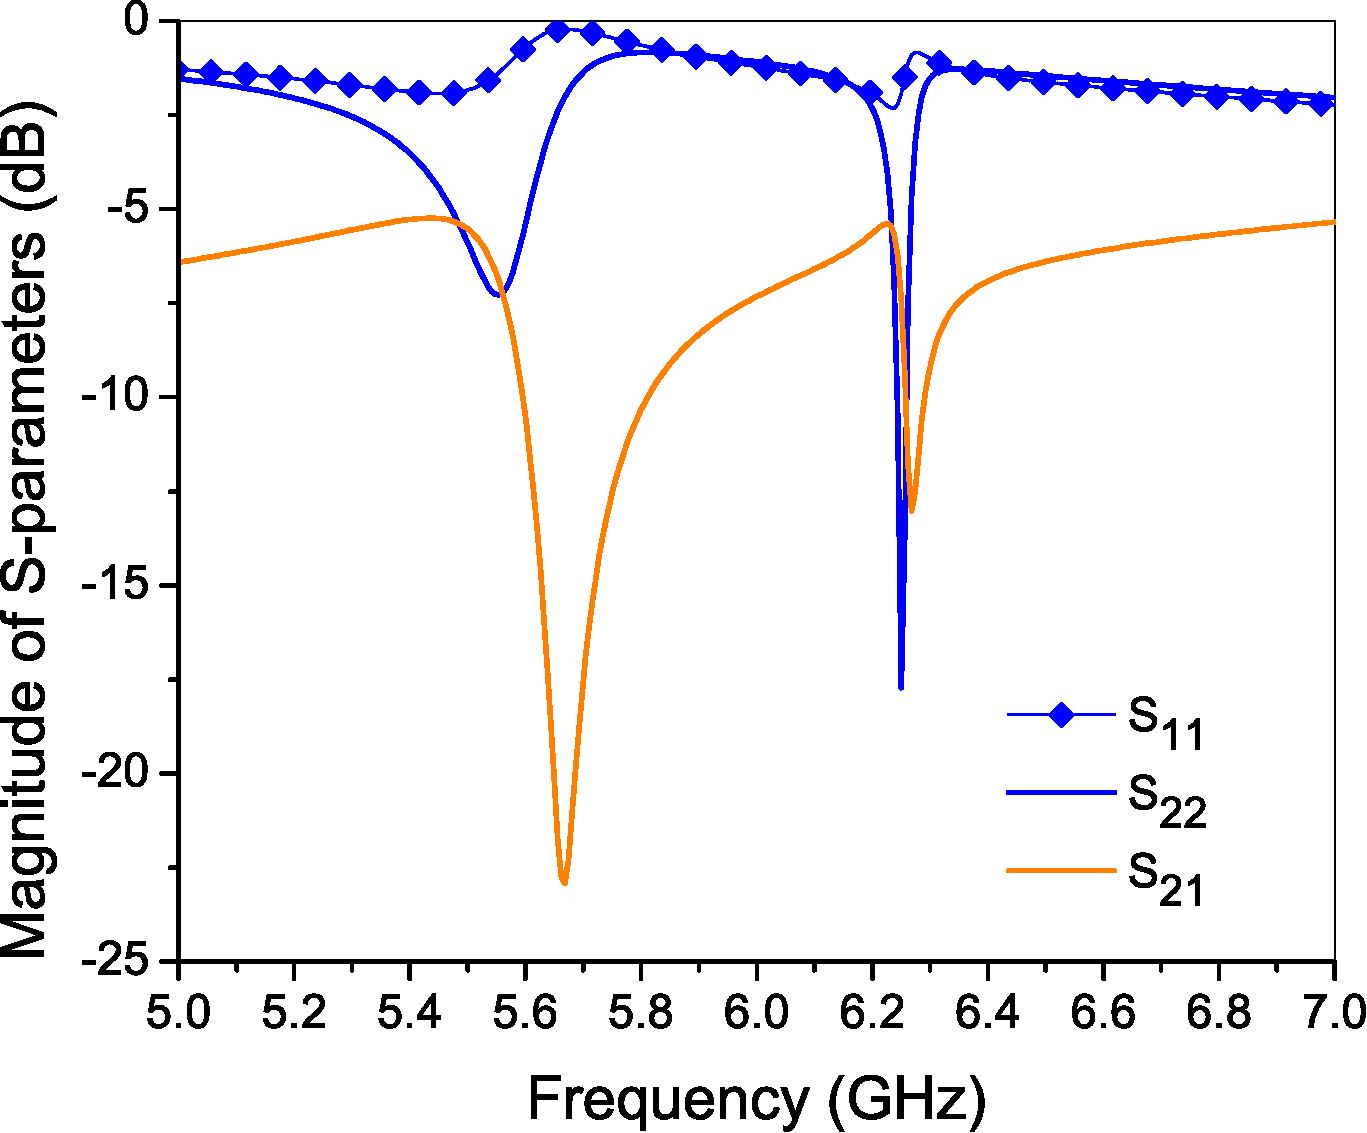
\includegraphics[width=0.45\textwidth]{slike/14a.pdf}
\label{fig14a}}
\hfill
\subfloat[]{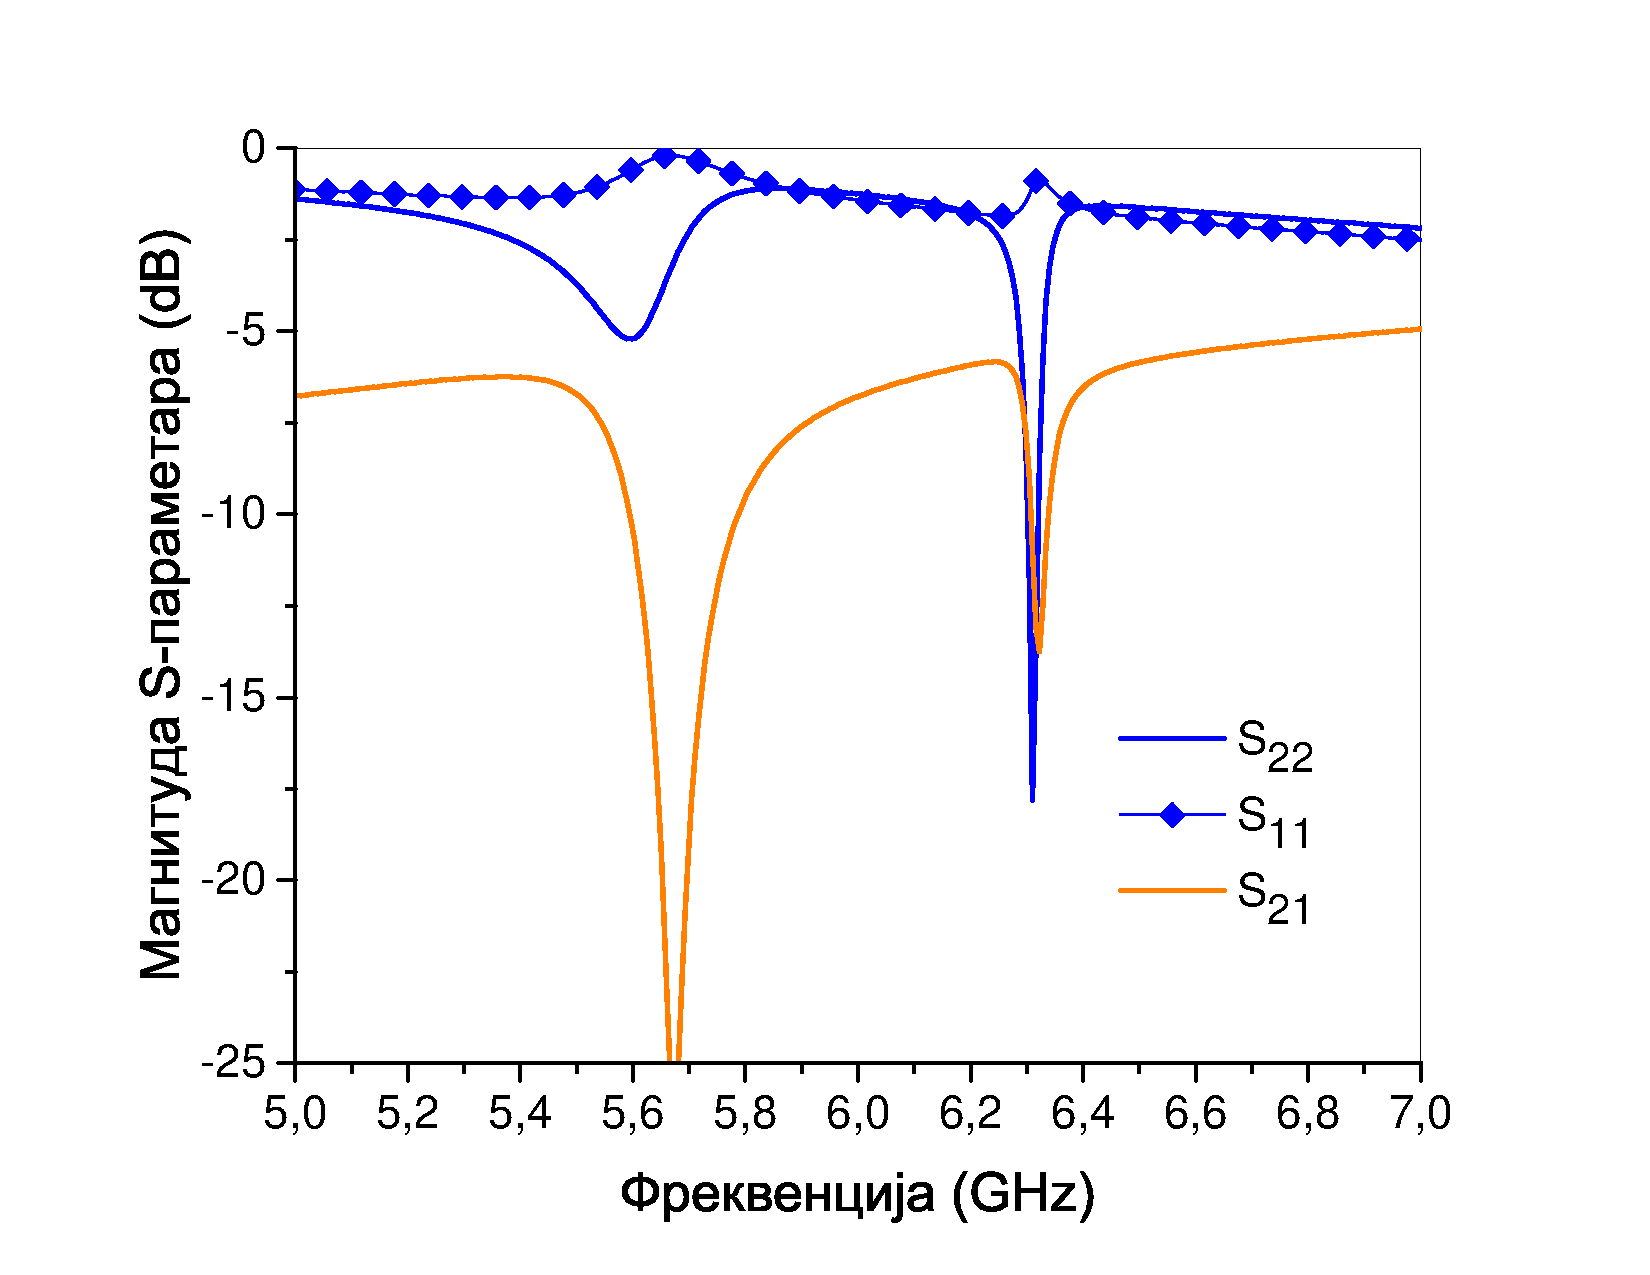
\includegraphics[width=0.45\textwidth]{slike/14b.pdf}
\label{fig14b}}
\caption{Магнитуда $Ѕ$-параметара за јединичне ћелије са нормалним процепом: (а) горњи процеп ближе воду, (б) даље од вода.}
\label{fig14_1}
\end{figure}
\begin{figure}[!t]
\centering
\subfloat[]{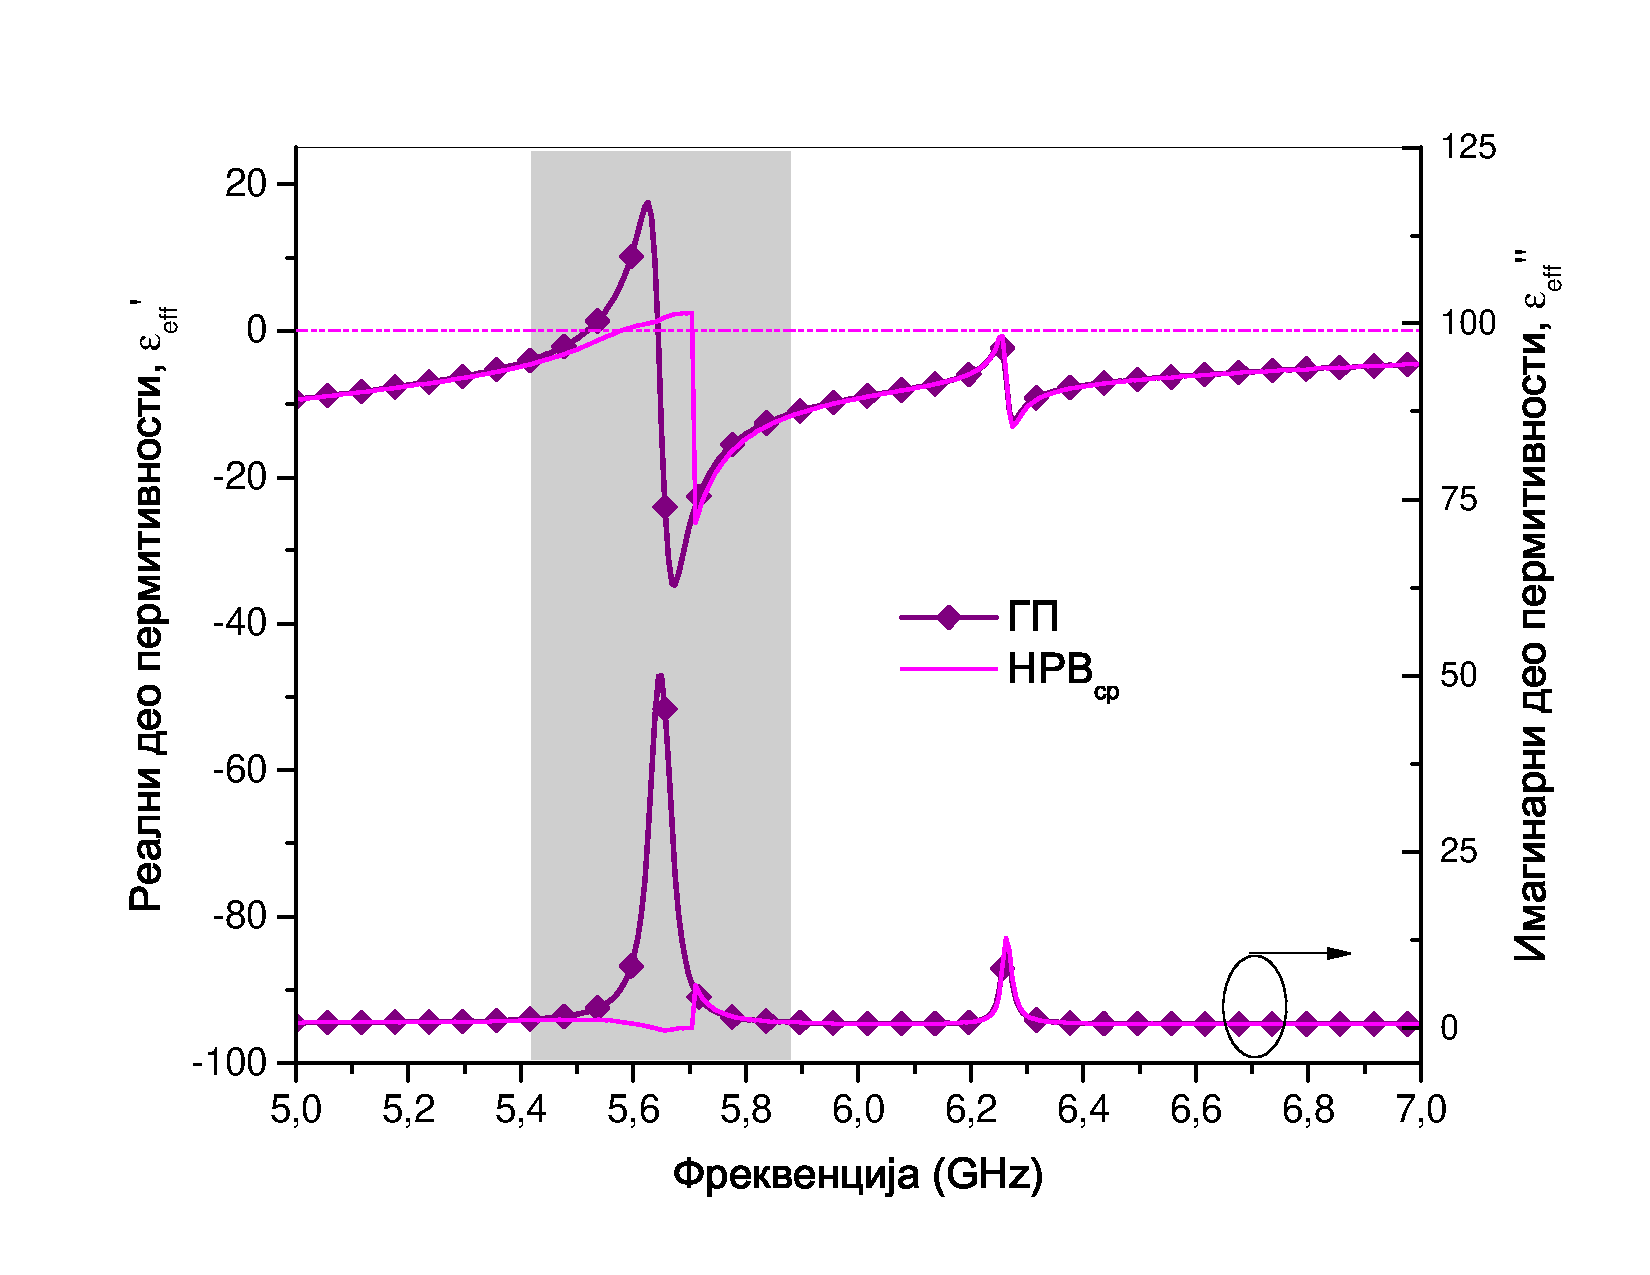
\includegraphics[width=0.5\textwidth]{slike/14c.pdf}
\label{fig14c}}\hfill
\subfloat[]{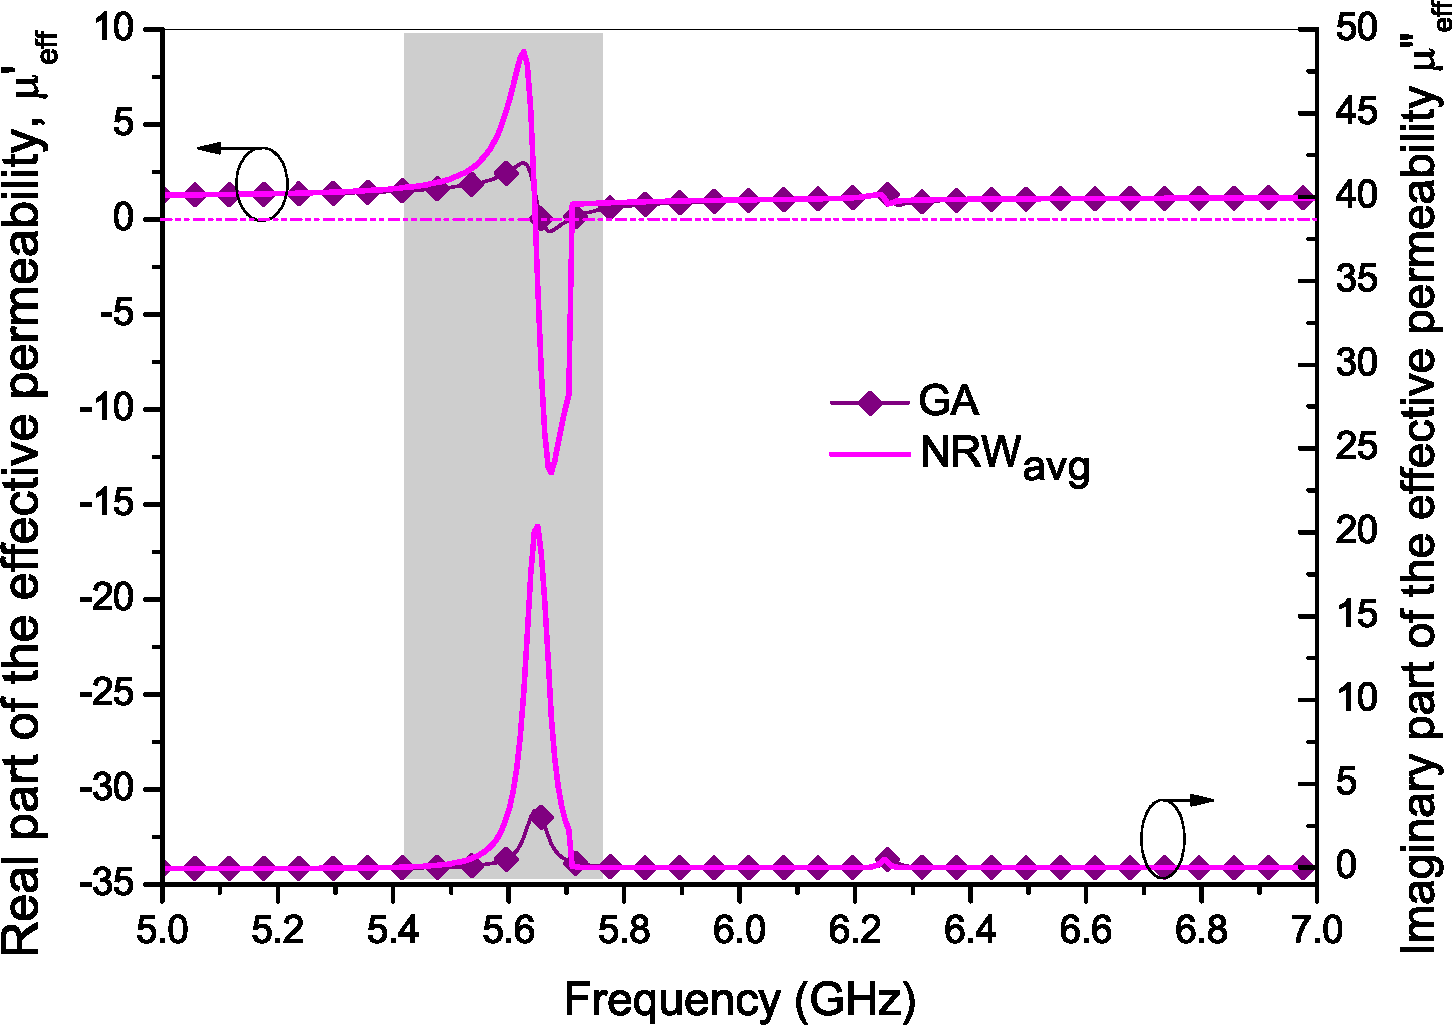
\includegraphics[width=0.5\textwidth]{slike/14e.pdf}
\label{fig14d}}
\caption{Ефективни параметри екстраховани ГП и $НРВ_{ср}$ методама за јединичне ћелије са горњим процепом ближе воду: (а) пермитивност, (б) пермеаблиност. Осенчени правоугаоници означавају зоне у којима две методе дају другачије резултате.}
\label{fig14_2}
\end{figure}
\begin{figure}[!t]
\centering
\subfloat[]{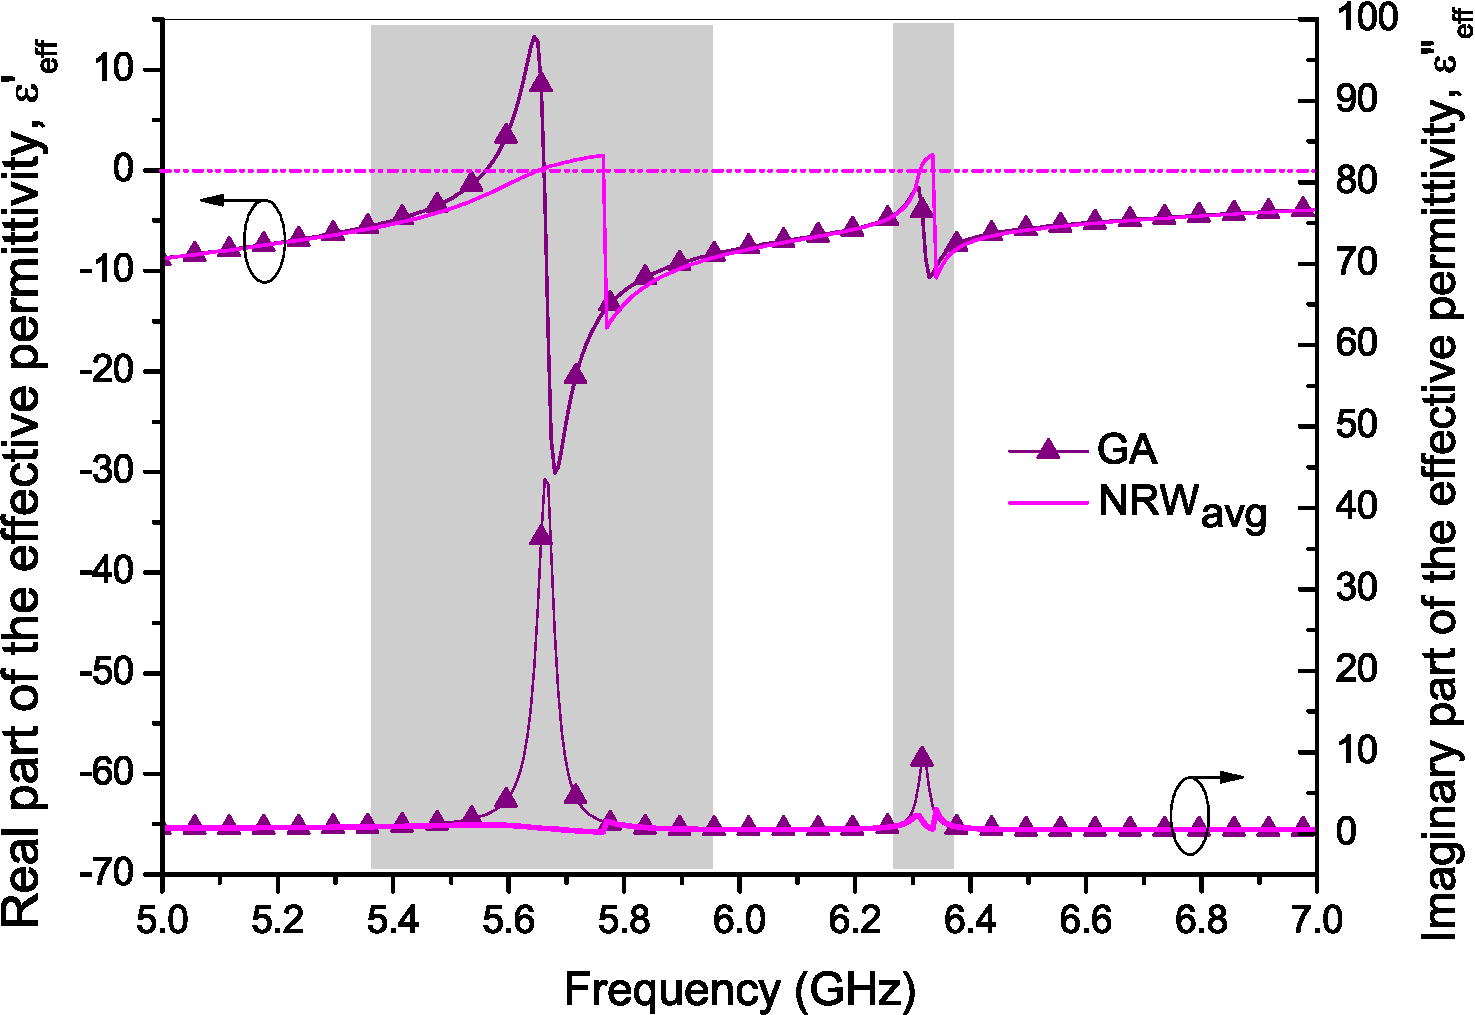
\includegraphics[width=0.6\textwidth]{slike/14d.pdf}
\label{fig14e}}\hfill
\subfloat[]{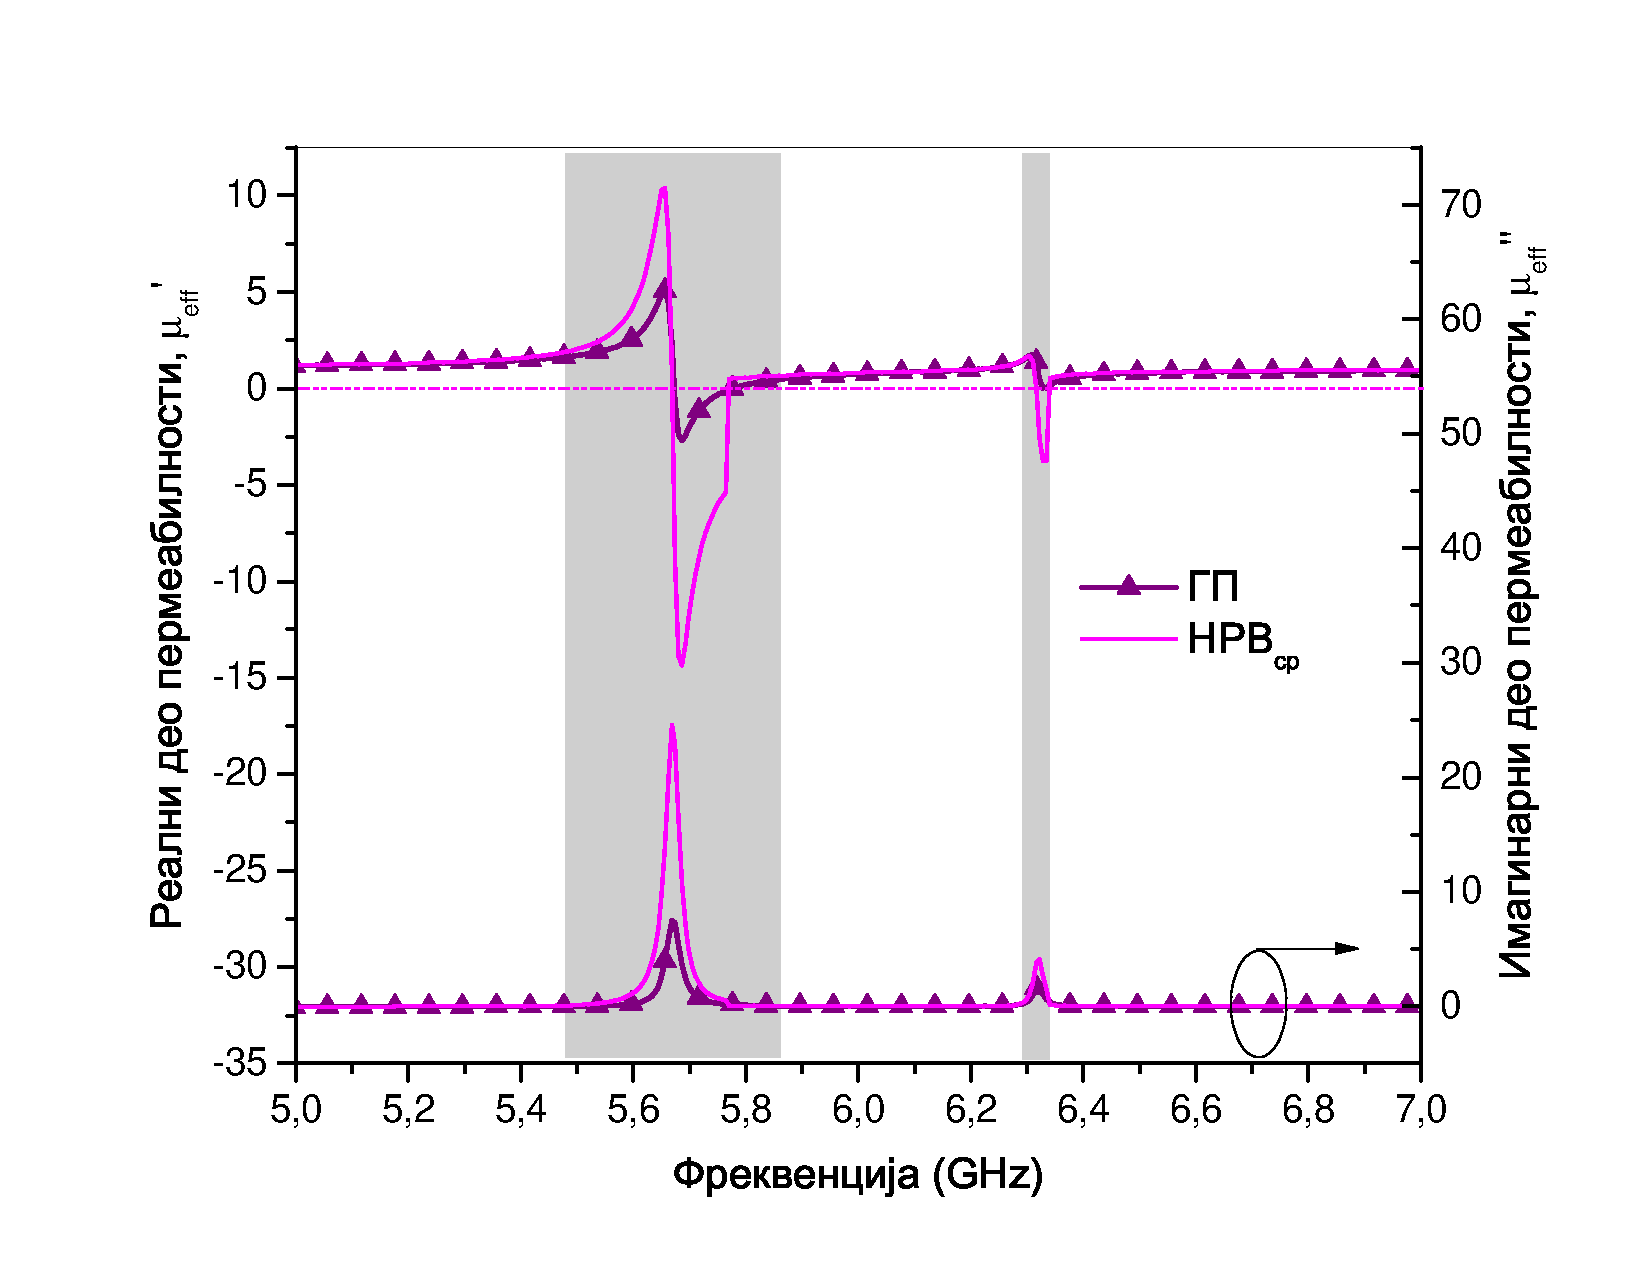
\includegraphics[width=0.6\textwidth]{slike/14f.pdf}
\label{fig14f}}
\caption{Ефективни параметри екстраховани ГП и $НРВ_{ср}$ методама за јединичне ћелије са горњим процепом даље од вода: (а) пермитивност, (б) пермеаблиност. Осенчени правоугаоници означавају зоне у којима две методе дају другачије резултате.}
\label{fig14_3}
\end{figure}

%It can be seen that asymmetry, i.e. difference in $S_{11}$ and $S_{22}$ exist around both resonances. The extracted effective parameters obtained by the two methods differ significantly especially around the first resonance due to the very strong asymmetry. This support our statement that averaged Nicolson-Ross-Weir based on averaging $S_{11}$ and $S_{22}$ is not suitable for highly asymmetric or bianisotropic unit cells.
%
Карактеристике јединичних ћелија са нормалним процепима су упоређене на сл.~\ref{fig15}. Може се видети да је реални део индекса преламања позитиван у целом опсегу за ћелију са процепом ближе воду, док за ћелију са процепом даље од вода поседује уски опсег са негативном вредношћу. Асиметрија је такође много израженија када је процеп даље од вода, као што је био случај и код ћелија са паралелним процепима. Код обе ћелије са нормалним процепима, максимална вредност параметра $u$ ($u_{даље}=8.6$ и $u_{ближе}=6.6$) је знатно већа него у случају са паралелним процепима ($u_{даље}=3.69$ and $u_{ближе}=1.21$).
\begin{figure}[!t]
\centering
\subfloat[]{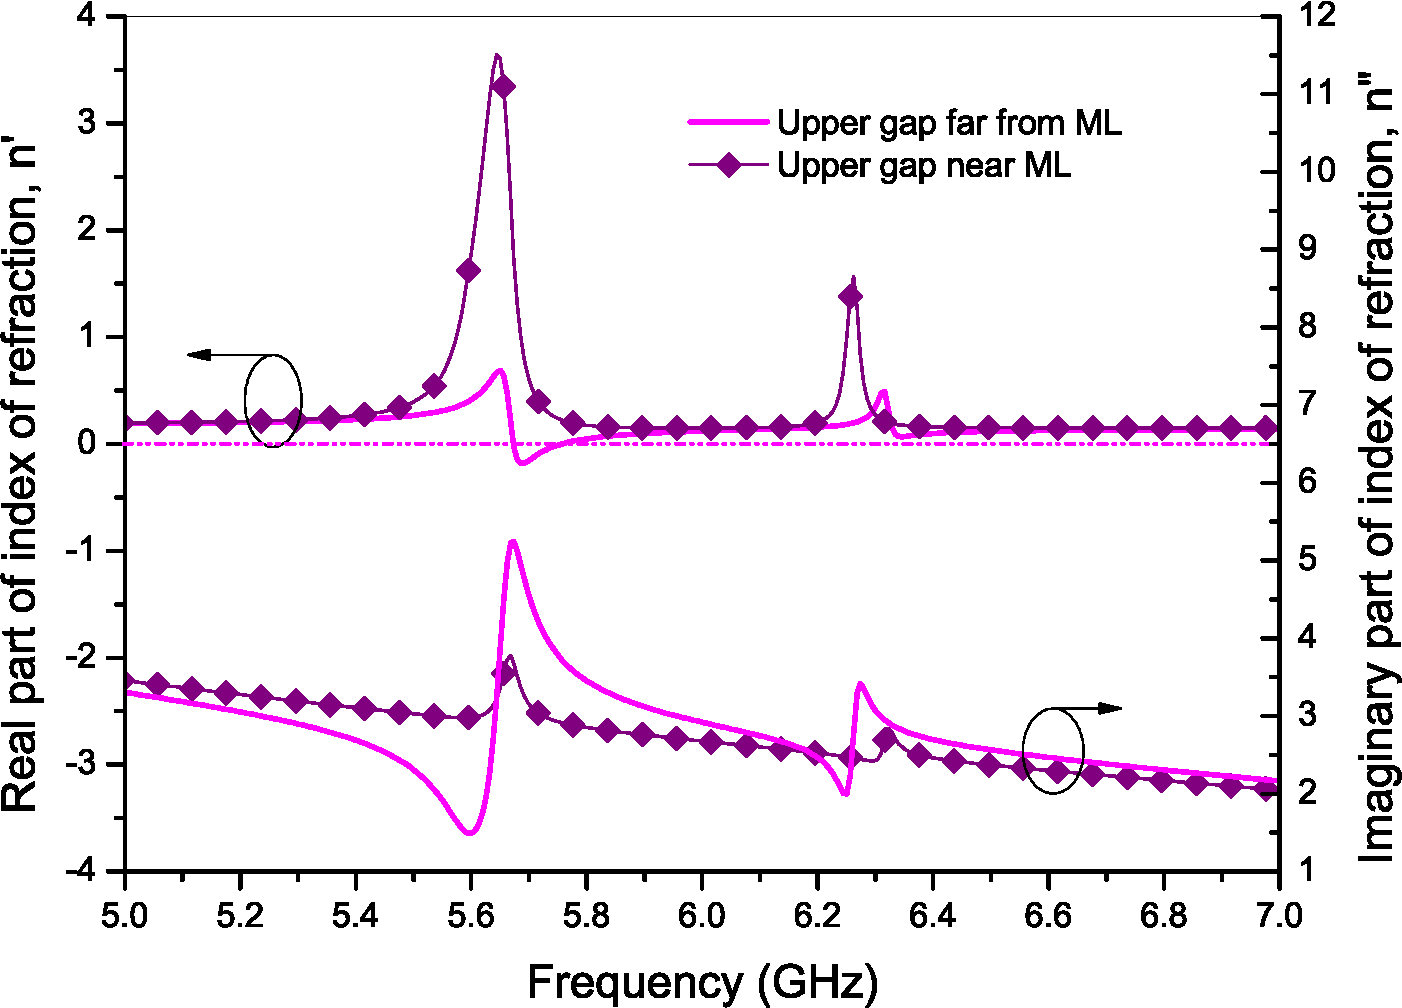
\includegraphics[width=0.6\textwidth]{slike/15a.pdf}
\label{fig15a}}
\subfloat[]{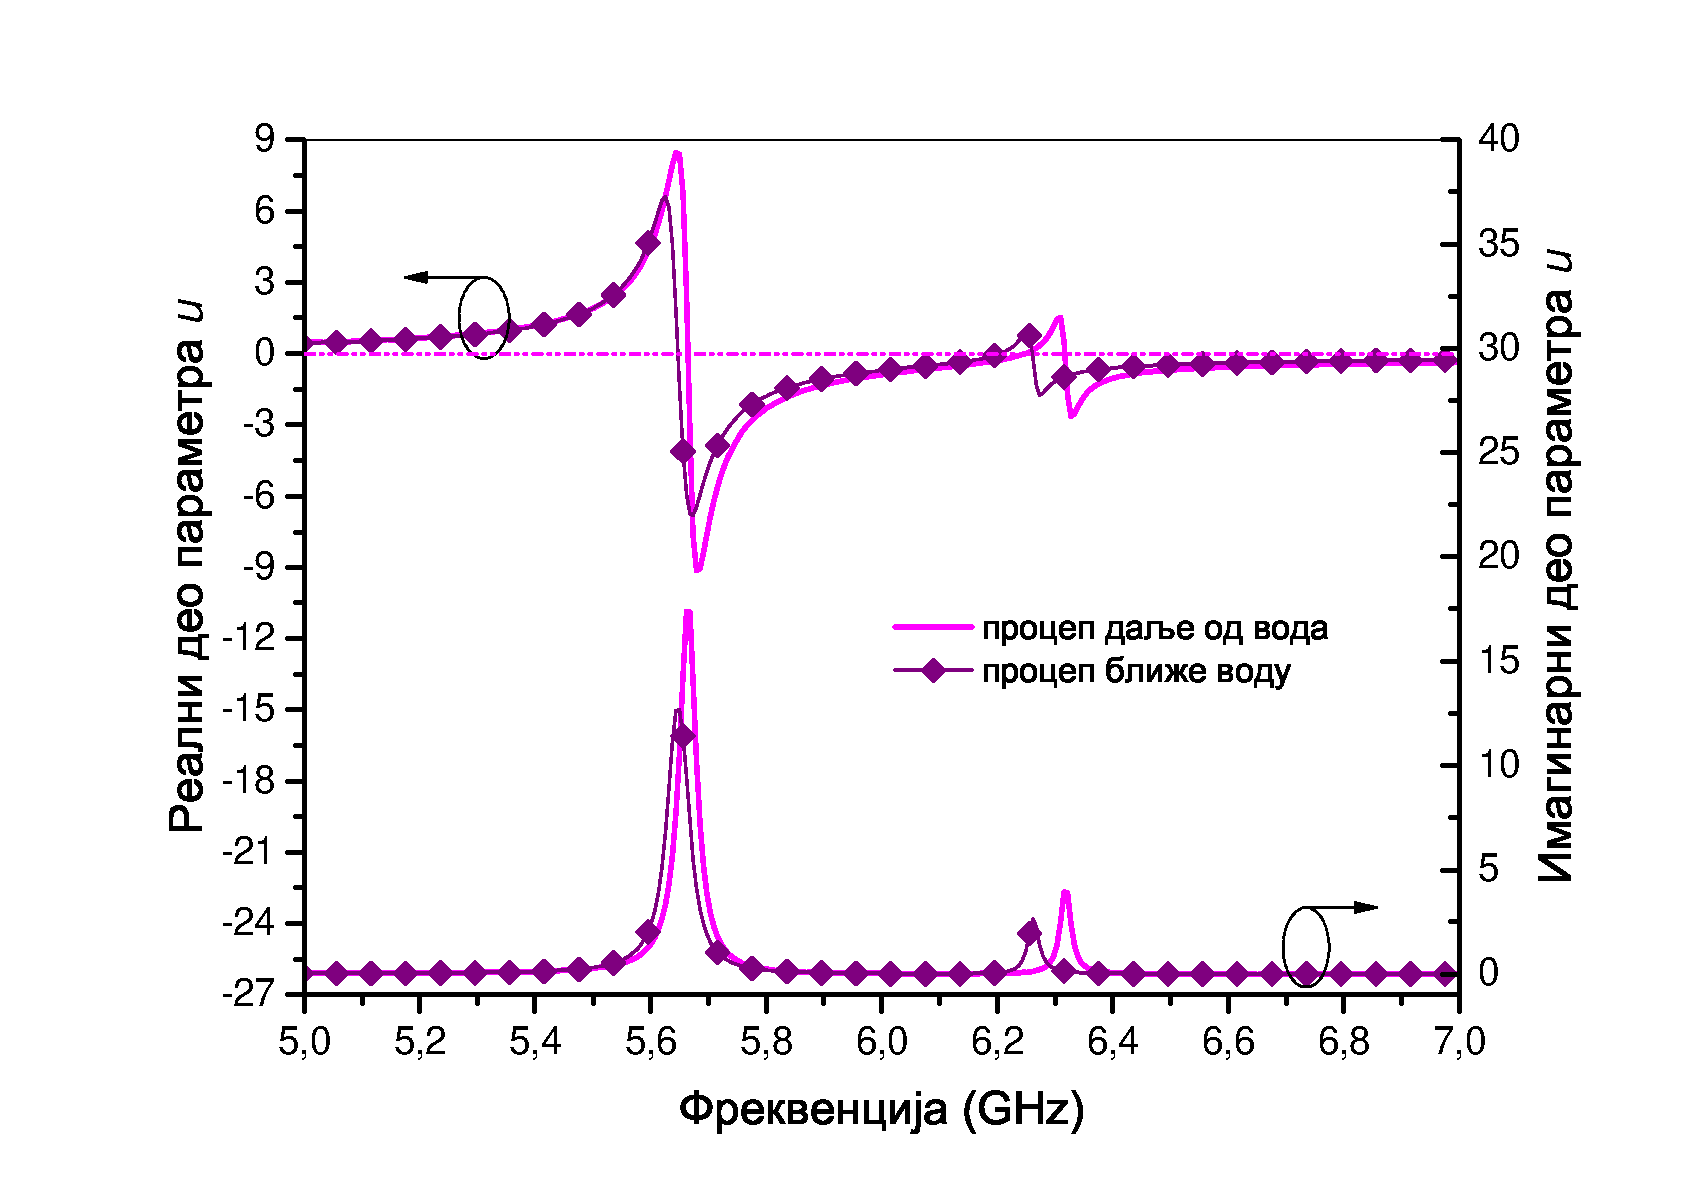
\includegraphics[width=0.6\textwidth]{slike/15b.pdf}
\label{fig15b}}

\caption{Екстраховани индекс преламања (а) и параметар $u$ (б) за јединичне ћелије са нормалним процепима.}
\label{fig15}
\end{figure}

На сл.~\ref{usl_norm} упоређени су стандардни услов за негативни индекс преламања и нови услов, за ћелије са горњим процепом даље од вода. За рачунање оба услова коришћени су параметри добијени ГП поступком. Може се видети да се, око прве резонансе, нови критеријум тачно поклапа са тачкама где реални део индекса пролази кроз нулу. То није случај са стандардним критеријумом, који предвиђа осетно већи опсег негативних вредност индекса. Око друге резонансе на 6.3\,GHz стандардни критеријум предвиђа негативне вредности, док је индекс заправо позитиван. Као доказ валидности новог критеријума додата је криву која одговара стандардном критеријуму, али срачунатом за параметре добијене $НРВ_{ср}$ методом, која се у потпуности поклапа са новим критеријумом.
\begin{figure}[!t]
\centering
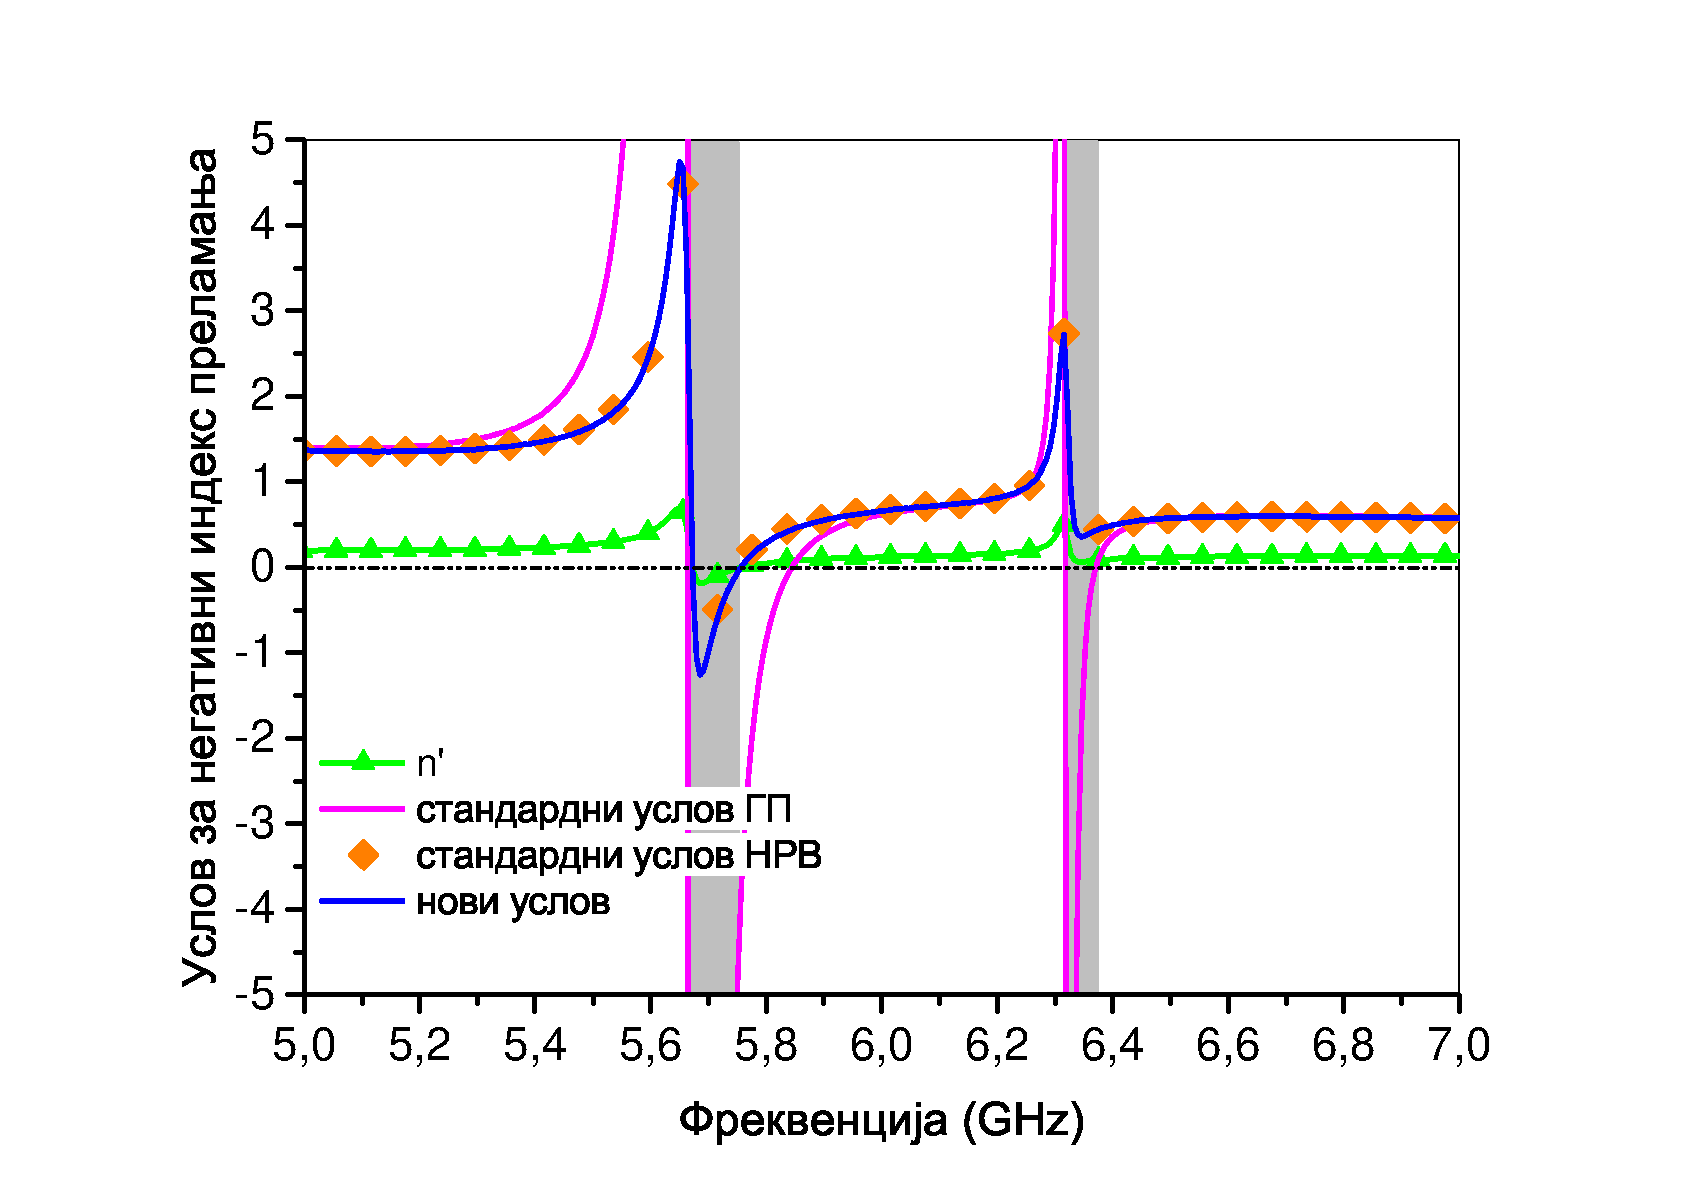
\includegraphics[scale=\SkalaC]{slike/usl_norm.pdf}
\caption{Поређење стандардног и новог критеријума за негативни индекс преламања, за ћелију са нормалним процепом даље од вода. Осенчене су зоне где ћелија има асиметрични одзив и два критеријума предвиђају различите опсеге негативних вредности.}
\label{usl_norm}
\end{figure}

\subsection{Ивично спрегнути СРР (\emph{физ.скрипта})}

\newcommand{\labelaslike}{а)~СРР са паралелним процепима, б)~СРР са нормалним процепима. }
(Такође су разматране)
На сл.~\ref{ph:fig1} приказане су структуре, са релевантним димензијама, код којих су коришћени ивично спрегнути (edge-coupled) СРР-ови. Код њих су прстенови постављени концентрично у истој равни, што знатно олакшава фабрикацију, пошто нема потребе за двослојним диелектриком. С друге стране, смањена је слобода приликом пројектовања. Поново су присутна два случаја, у зависности од тога да ли су процепи оријентисани паралелно (\ref{ph:fig1a}) или нормално (\ref{ph:fig1b}) у односу на вод.
\begin{figure}[!t]
\centering
\subfloat[]{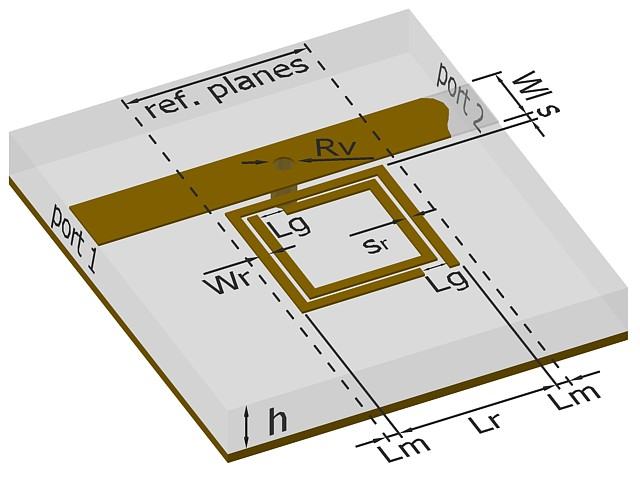
\includegraphics[width=0.45\textwidth]{slike/physcr/pod0/model.jpeg}
\label{ph:fig1a}}
\hfill
\subfloat[]{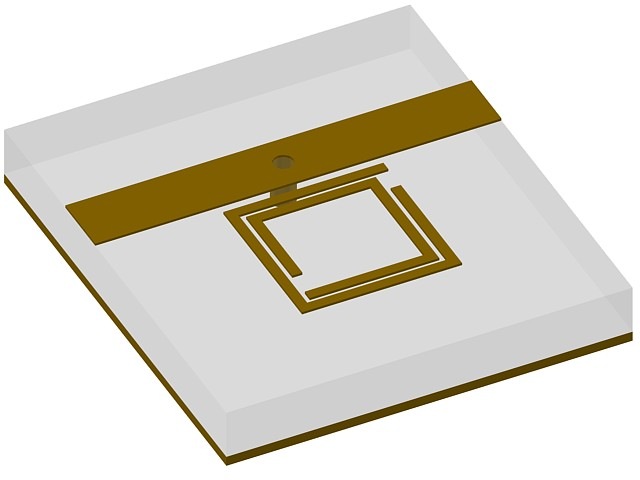
\includegraphics[width=0.45\textwidth]{slike/physcr/pod90/model.jpeg}
\label{ph:fig1b}}
\caption{Ћелије са ивично спрегнутим СРР-овима: \labelaslike Релевантне димензије: $h=\num{1.27}\,\mathrm{mm}$, $L_r=3\,\mathrm{mm}$, $L_g=\num{0.5}\,\mathrm{mm}$, $L_m=\num{0.25}\,\mathrm{mm}$, $W_l=\num{1.2}\,\mathrm{mm}$, $W_r=\num{0.2}\,\mathrm{mm}$, $R_v=\num{0.5}\,\mathrm{mm}$, $s=\num{0.1}\,\mathrm{mm}$, $s_r=\num{0.1}\,\mathrm{mm}$, и релативна пермитивност супстрата $\varepsilon_r=\num{10.2}$.}
\label{ph:fig1}
\end{figure} 

\begin{figure}[!t]
\centering
\subfloat[]{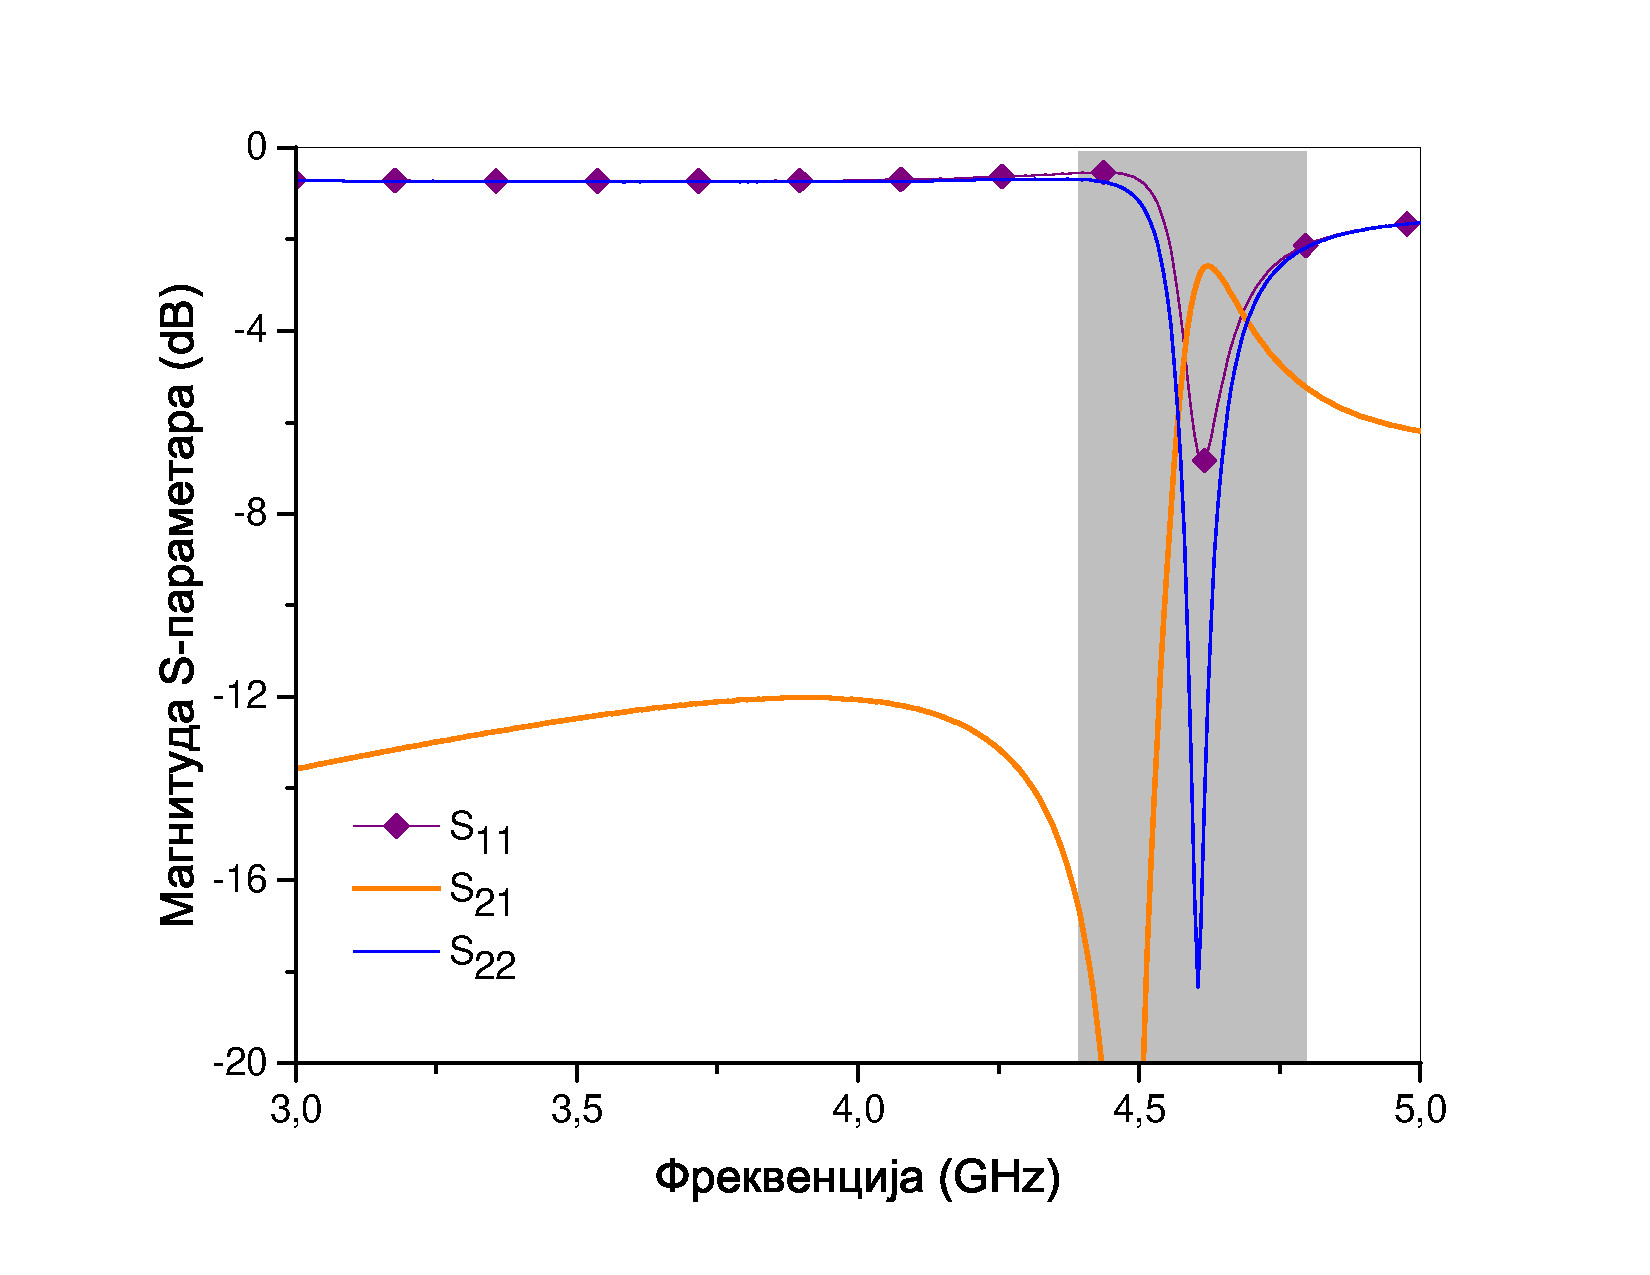
\includegraphics[width=0.48\textwidth]{slike/physcr/pod0/smag}}
%\label{fig}}
\hfill%\hspace*{1cm}
\subfloat[]{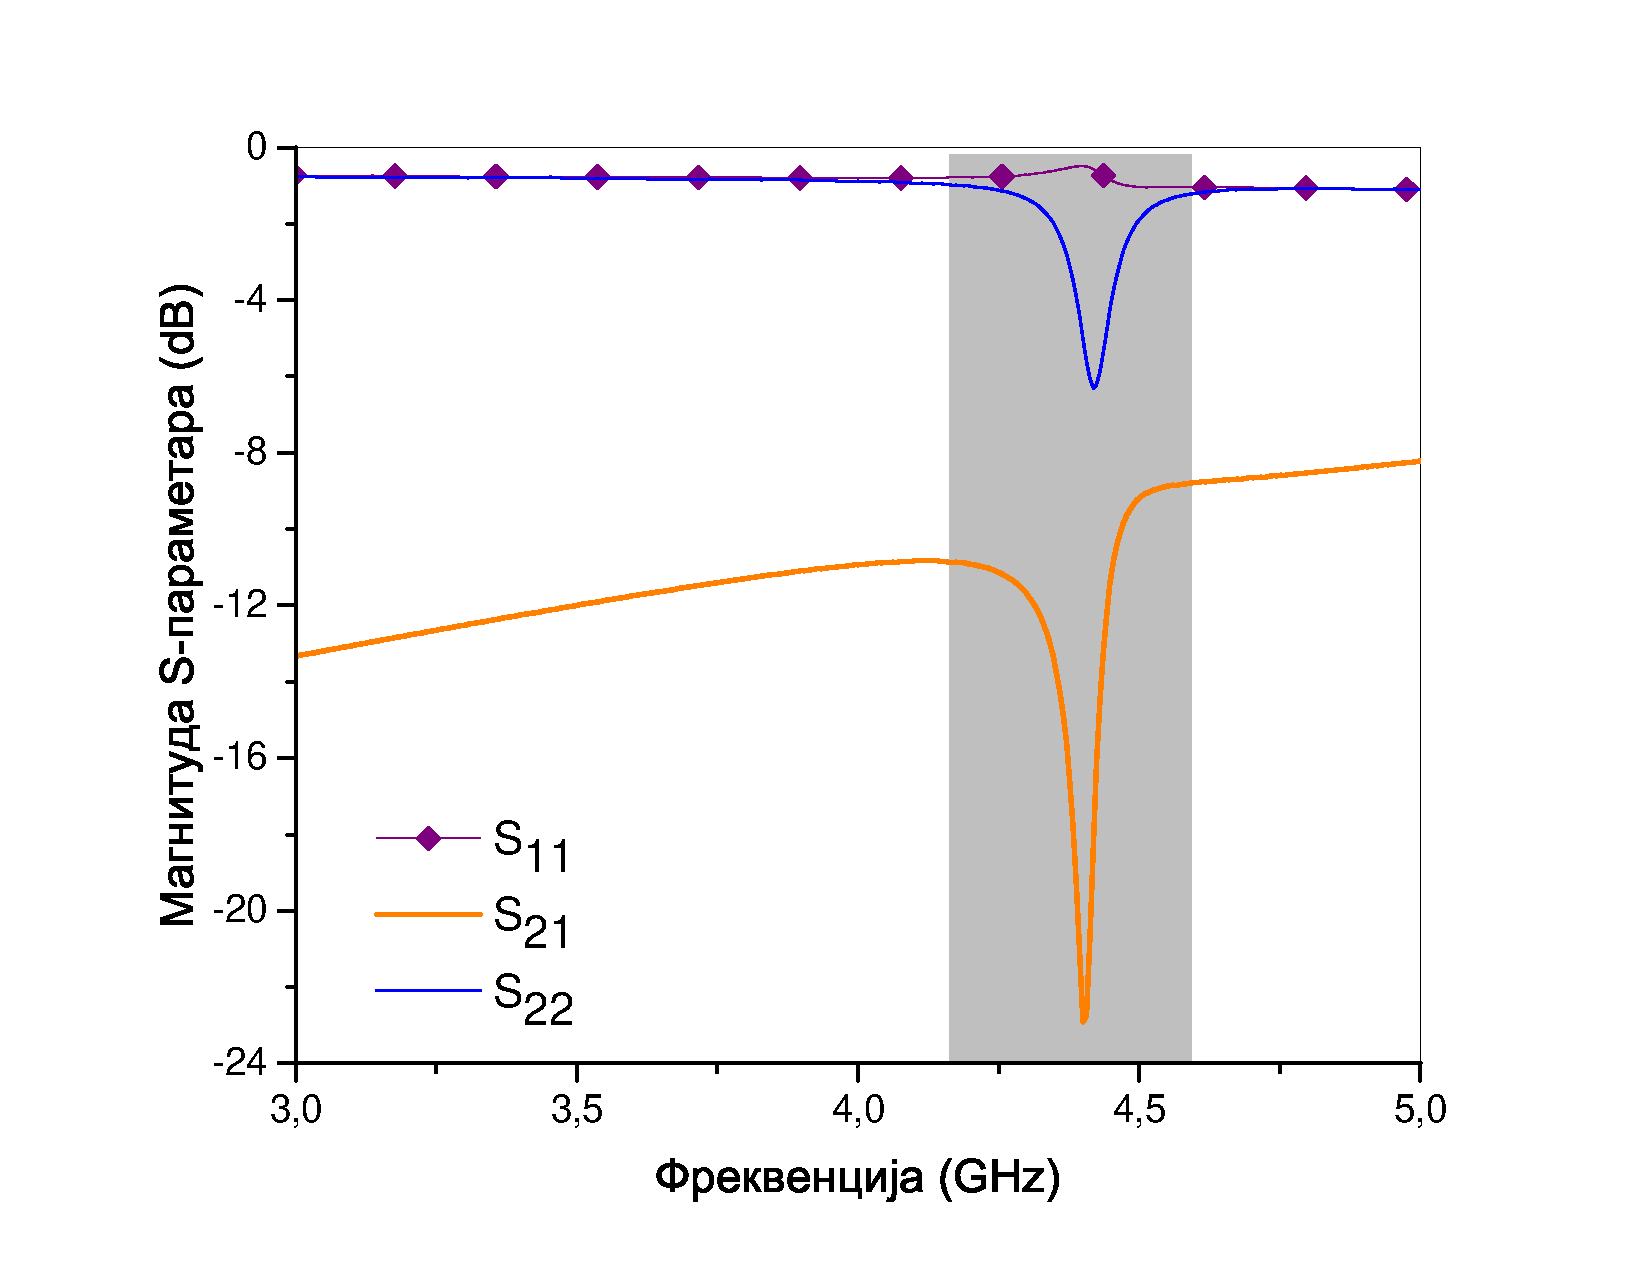
\includegraphics[width=0.48\textwidth]{slike/physcr/pod90/smag}}
%\label{fig}}
\caption{Магнитуда $S$-параметара: \labelaslike Асиметрија је присутна у осенченим деловима.}
\label{ph:fig2}
\end{figure} 

\begin{figure}[!t]
\centering
\subfloat[]{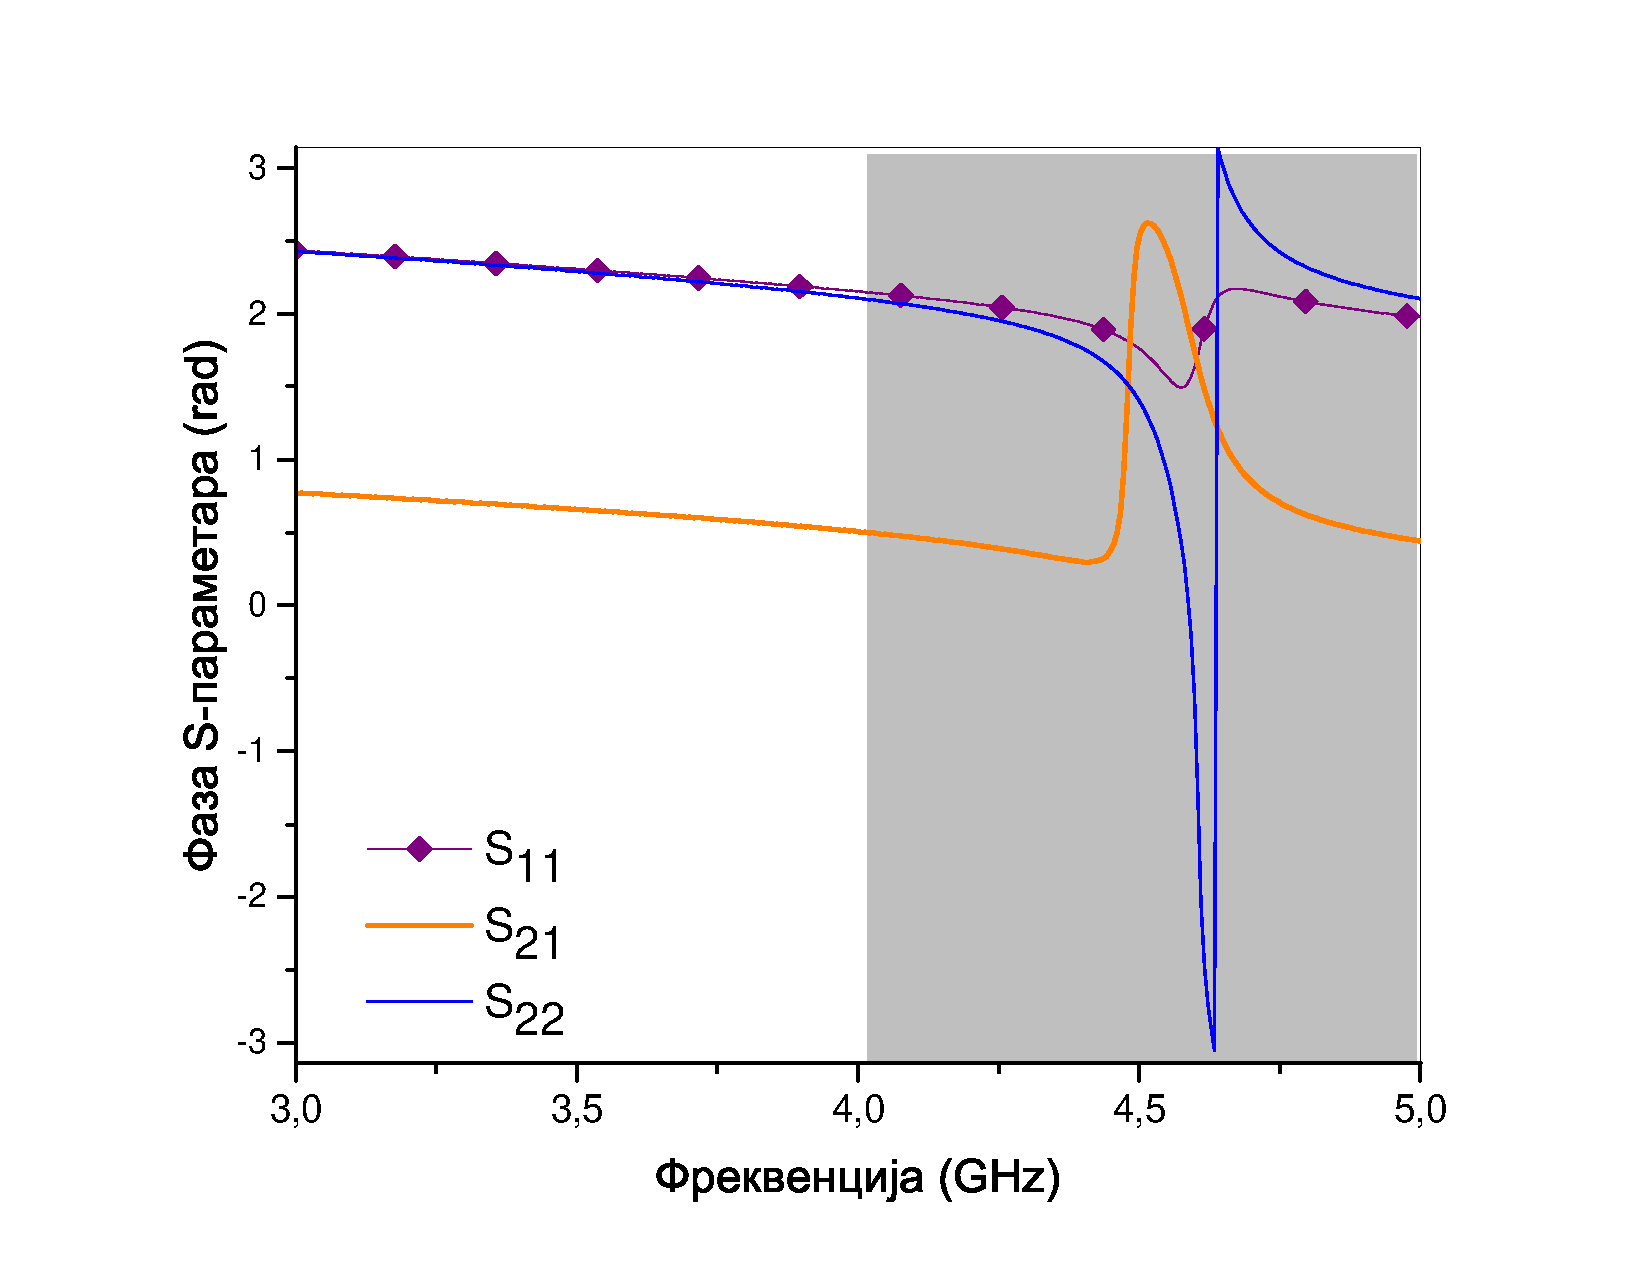
\includegraphics[width=0.48\textwidth]{slike/physcr/pod0/sfaza}}
%\label{fig}}
%\hspace*{1cm}
\subfloat[]{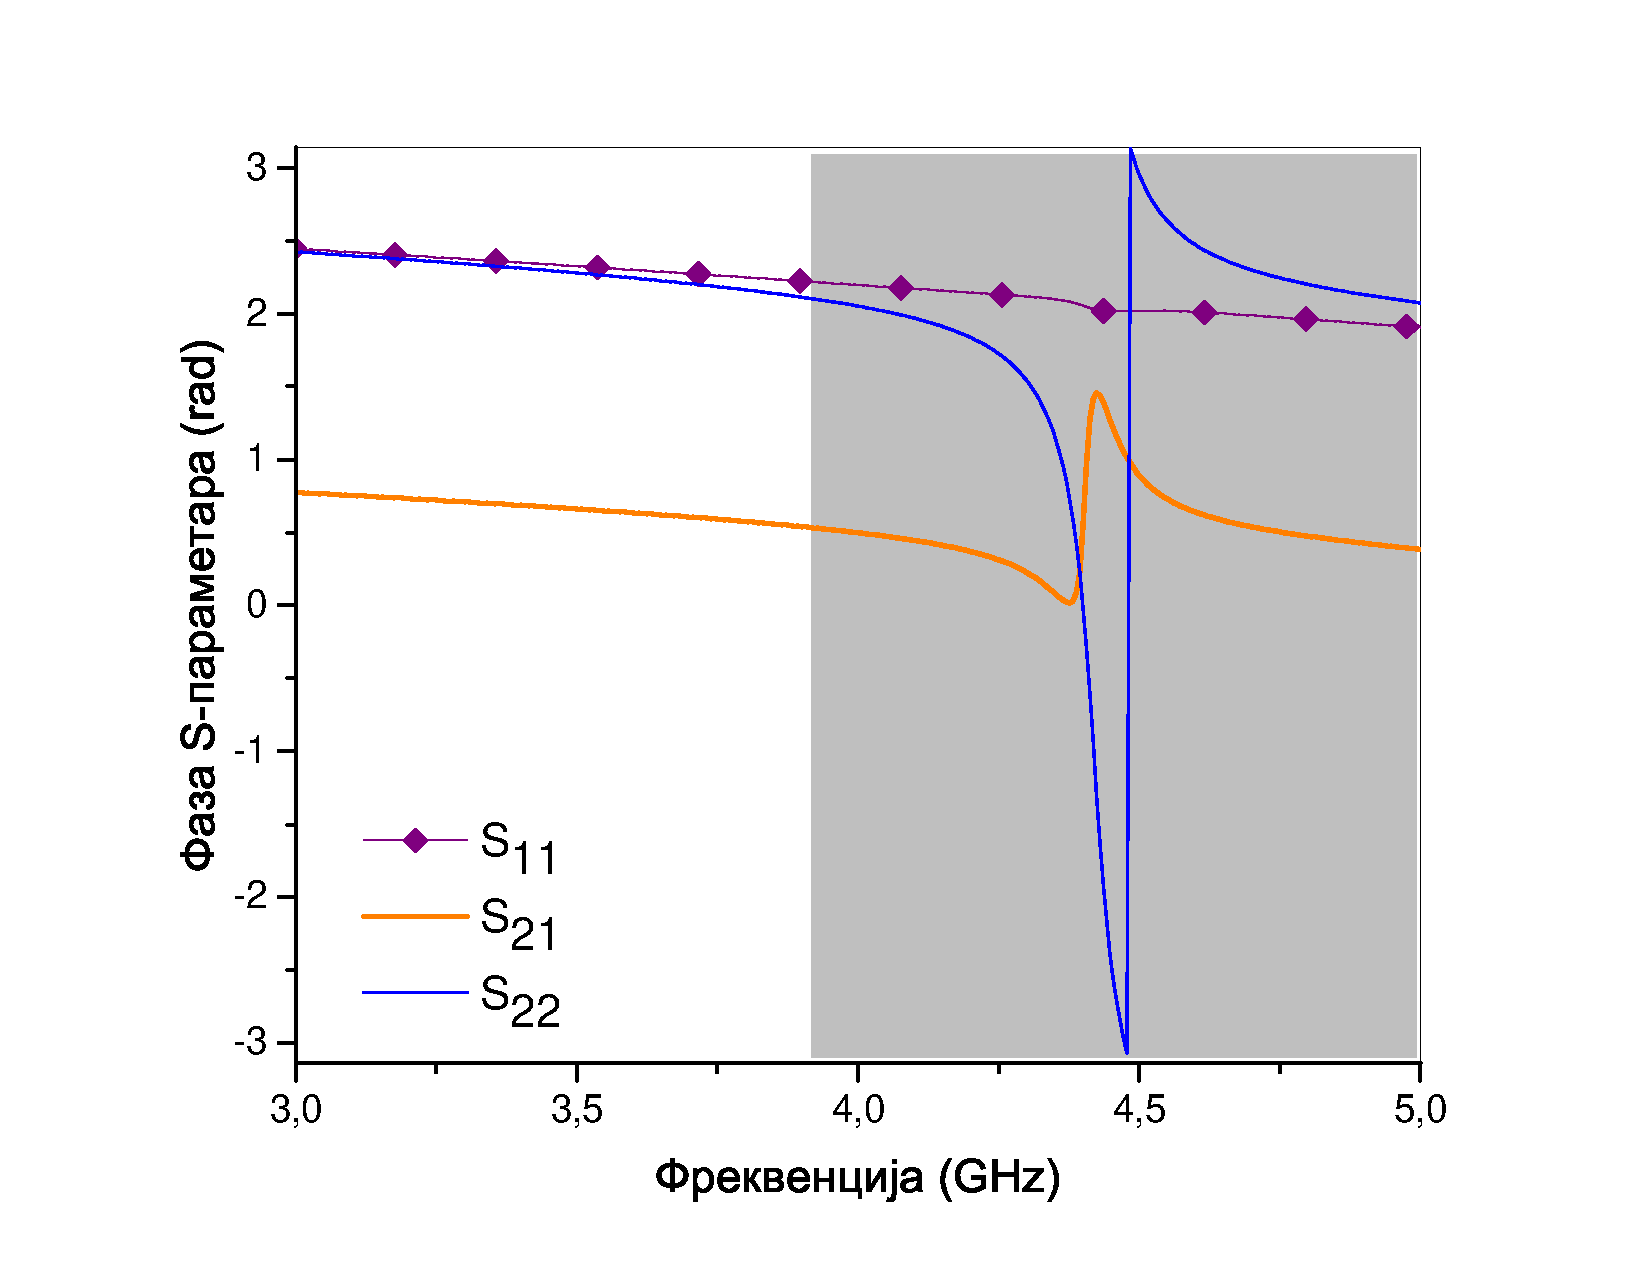
\includegraphics[width=0.48\textwidth]{slike/physcr/pod90/sfaza}}
%\label{fig}}
\caption{Фаза $S$-параметара: \labelaslike Асиметрија је присутна у осенченим деловима.}
\label{ph:fig3}
\end{figure} 
Симулирани $Ѕ$-параметри приказани су на сл.~\ref{ph:fig2}-\ref{ph:fig3}; види се да је асиметрија присутна само око резонанси, при чему је много израженија за случај са нормалним процепима са сл.~\ref{ph:fig1b}. Екстраховани ефективни параметри -- индекс преламања, карактеристична импеданса, пермитивност и пермеабилност дати су на сл.~\ref{ph:fig4}-\ref{ph:fig7}.

На сл.~\ref{ph:fig5} види се да карактеристична импеданса за $НРВ_{ср}$ има потпуно другачији облик и вредности од средње вредности за ГП метод, при чему за обе структуре испољава неприродно понашање (скокове) у околини резонансе. Ово ће резултовати неприродним обликом фреквенцијских зависности $\varepsilon$ и $\mu$, што се може видети на сл.~\ref{ph:fig6b} и \ref{ph:fig7b}.

Асиметрија је слабије изражена код структуре са паралелним процепима, што доводи до мање разлике у екстрахованим параметрима за два различита смера, што се види на сл.~\ref{ph:fig6a} and \ref{ph:fig7a}. У овом случају су резултати за $НРВ_{ср}$ изостављени пошто немају значајне разлике у односу на ГП. Насупрот томе, у случају са нормалним процепима асиметрија је наглашенија, због чега се импедансе за $ГП_1$ и $ГП_2$ значајније разликују, што последично изазива разлике и у ефективним параметрима, сл.~\ref{ph:fig6b} и \ref{ph:fig7b}.
\begin{figure}[!t]
\centering
\subfloat[]{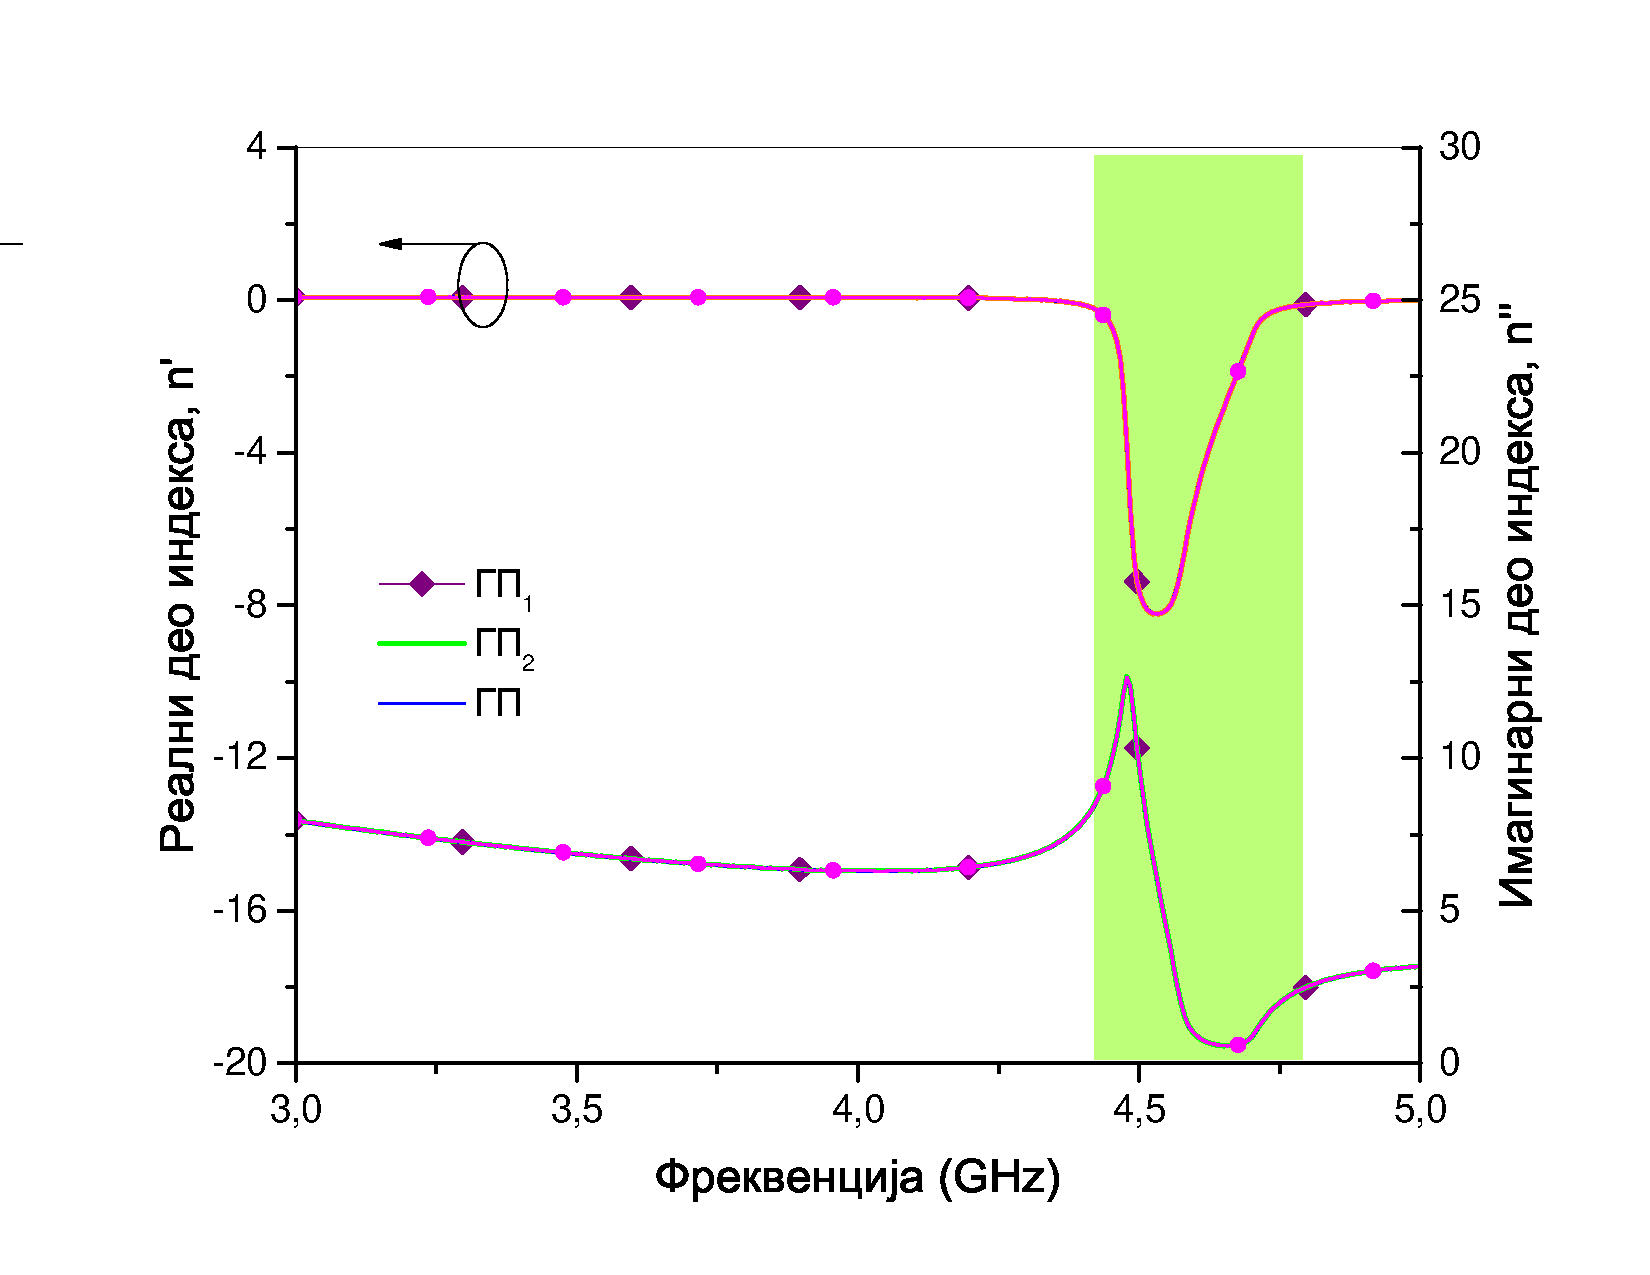
\includegraphics[width=0.6\textwidth]{slike/physcr/pod0/n}}
%\label{fig}}
\hfill
\subfloat[]{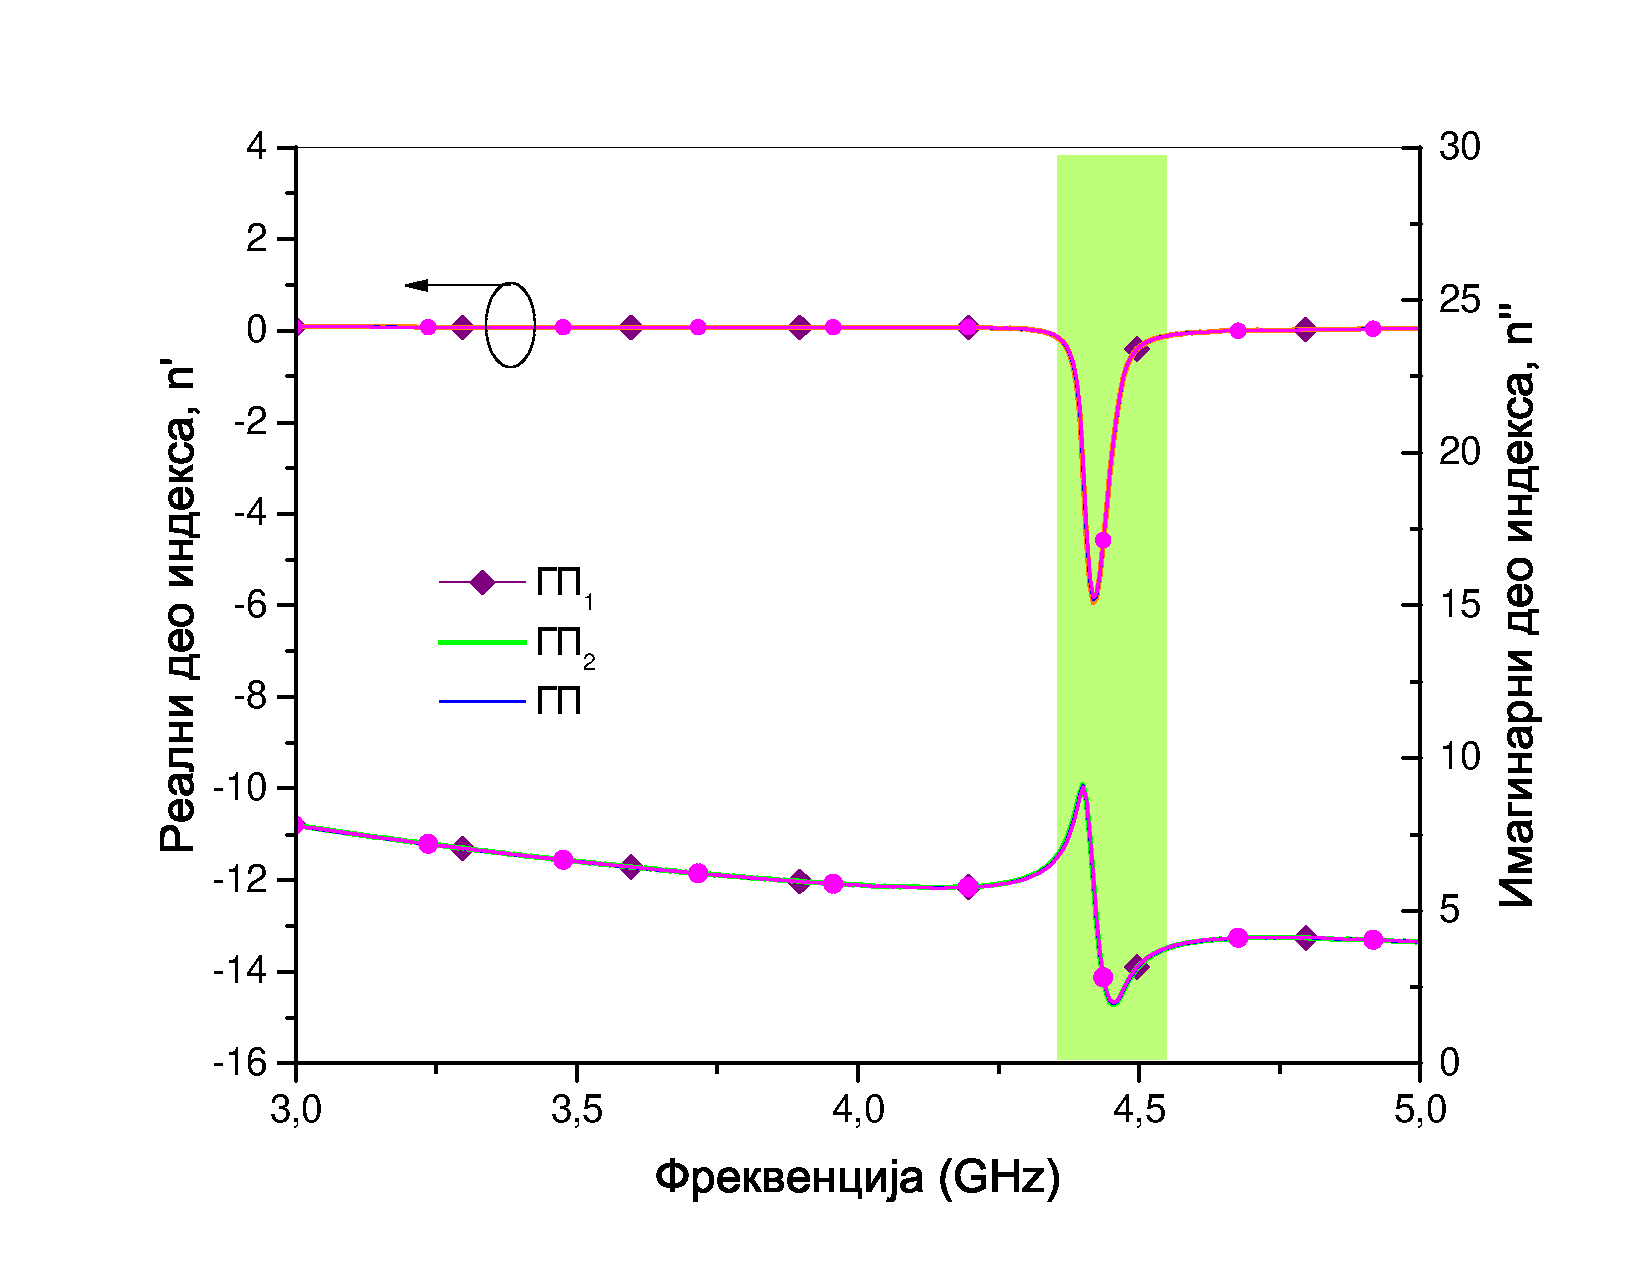
\includegraphics[width=0.6\textwidth]{slike/physcr/pod90/n}}
%\label{fig}}
\caption{Екстраховани индекс преламања: \labelaslike Осенчени делови означавају зоне са двоструко-негативним параметрима.}
\label{ph:fig4}
\end{figure} 

\begin{figure}[!t]
\centering
\subfloat[]{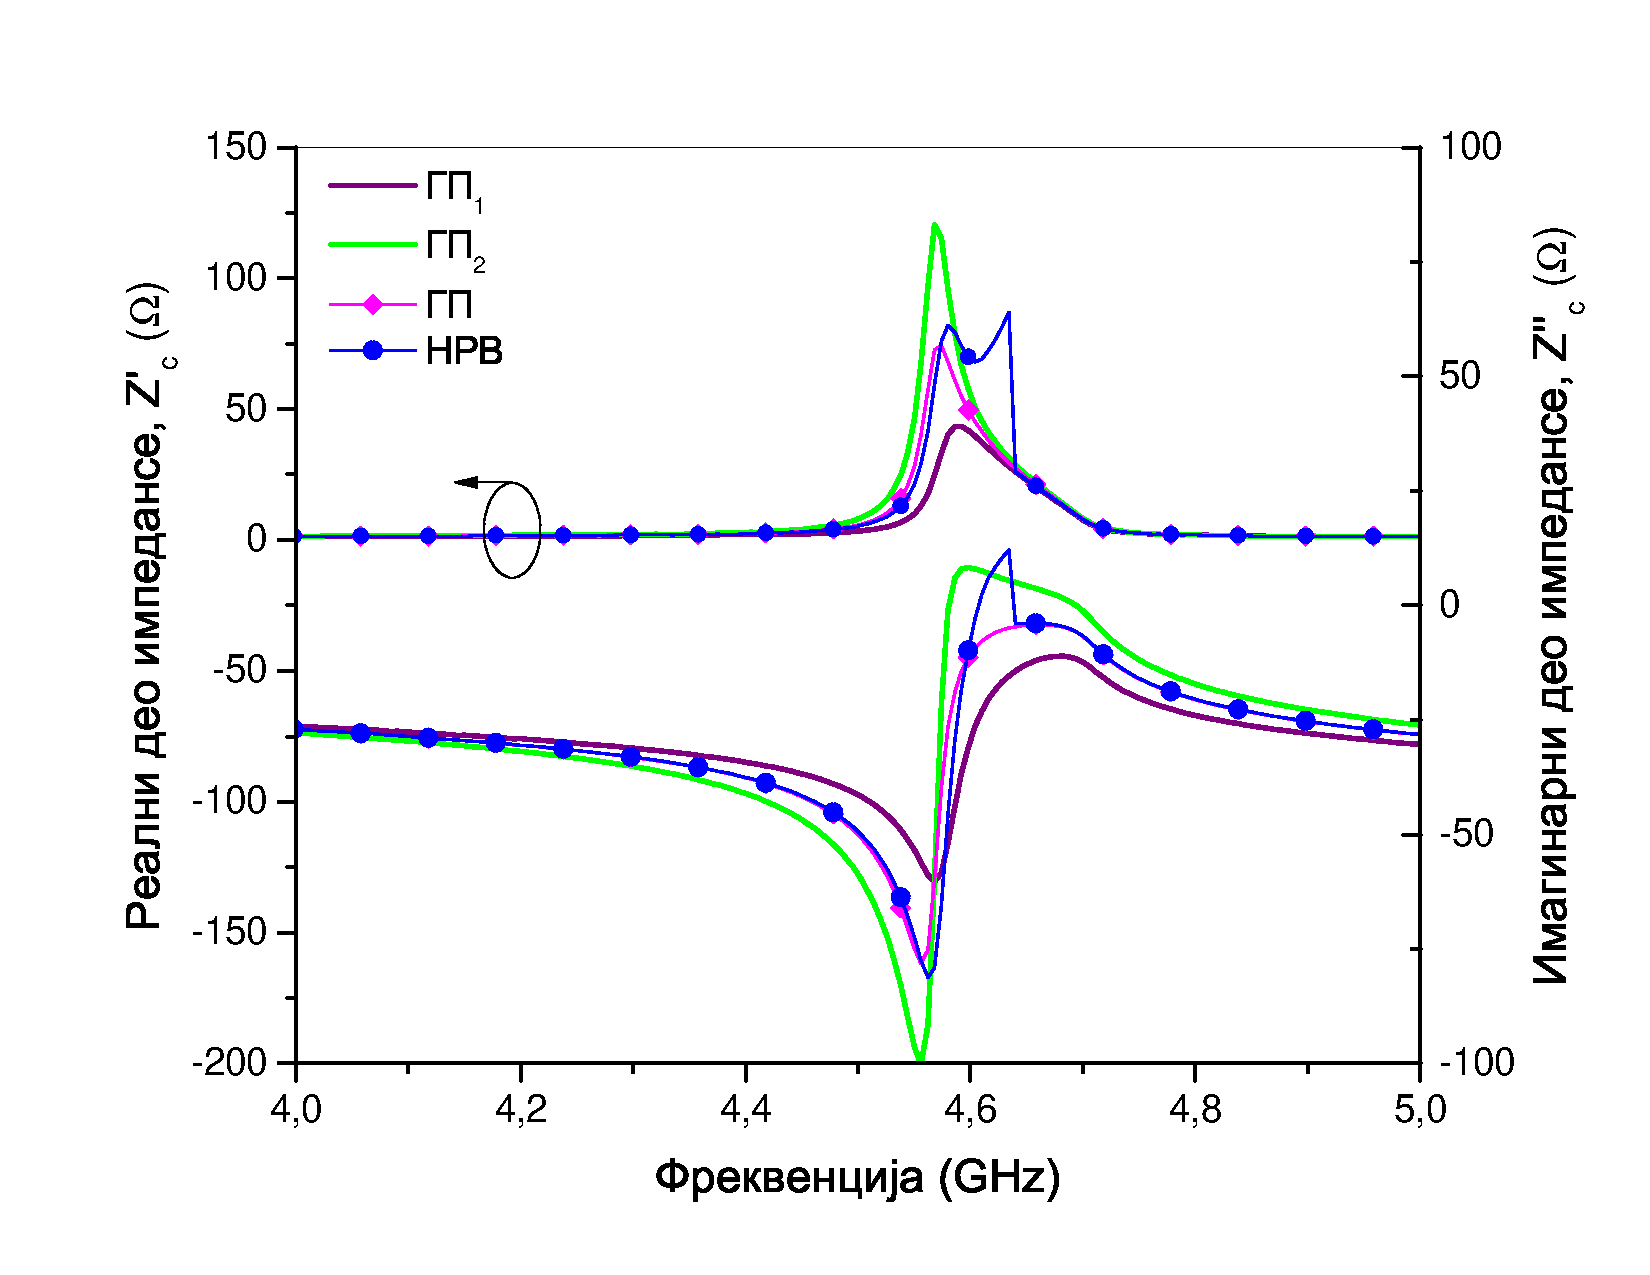
\includegraphics[width=0.6\textwidth]{slike/physcr/pod0/zc}}
%\label{fig}}
\hfill
\subfloat[]{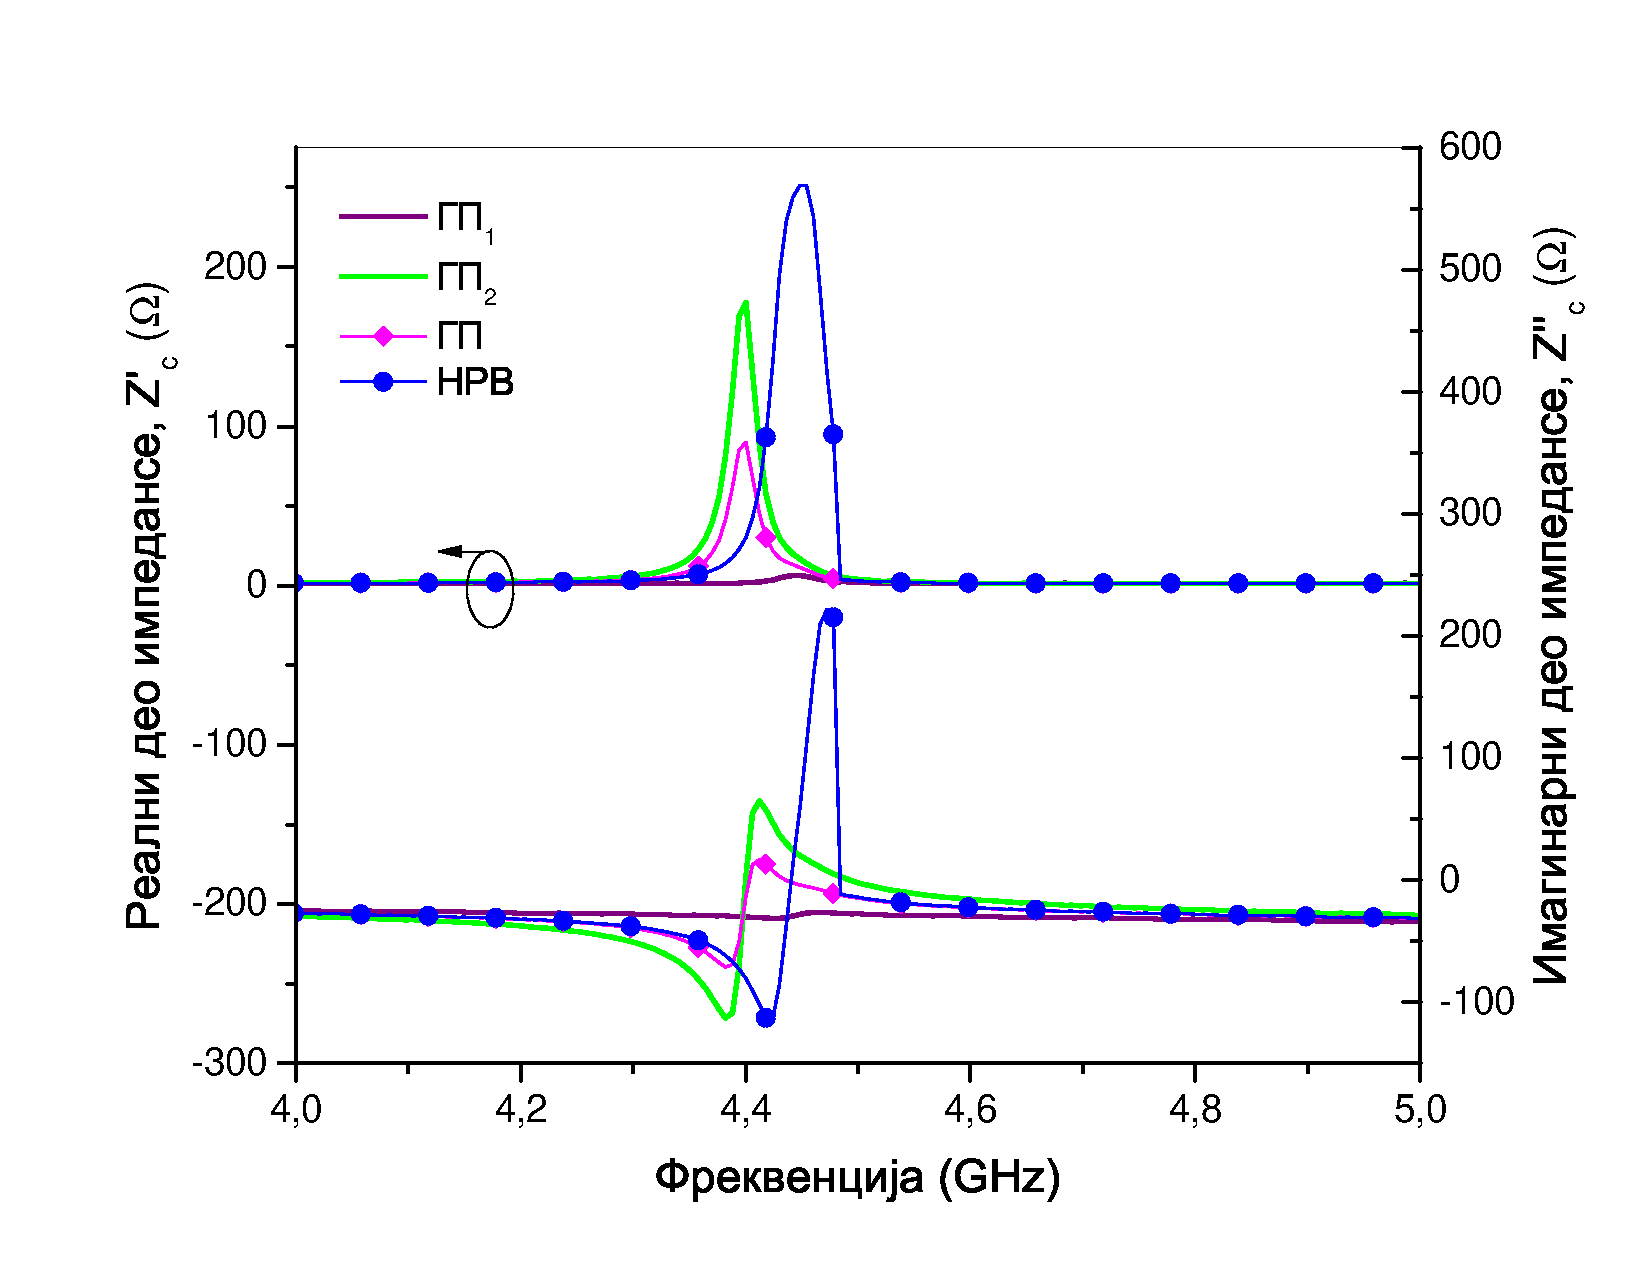
\includegraphics[width=0.6\textwidth]{slike/physcr/pod90/zc}}
%\label{fig}}
\caption{Екстрахована карактеристична импеданса: \labelaslike}
\label{ph:fig5}
\end{figure} 

\begin{figure}[!t]
\centering
\subfloat[]{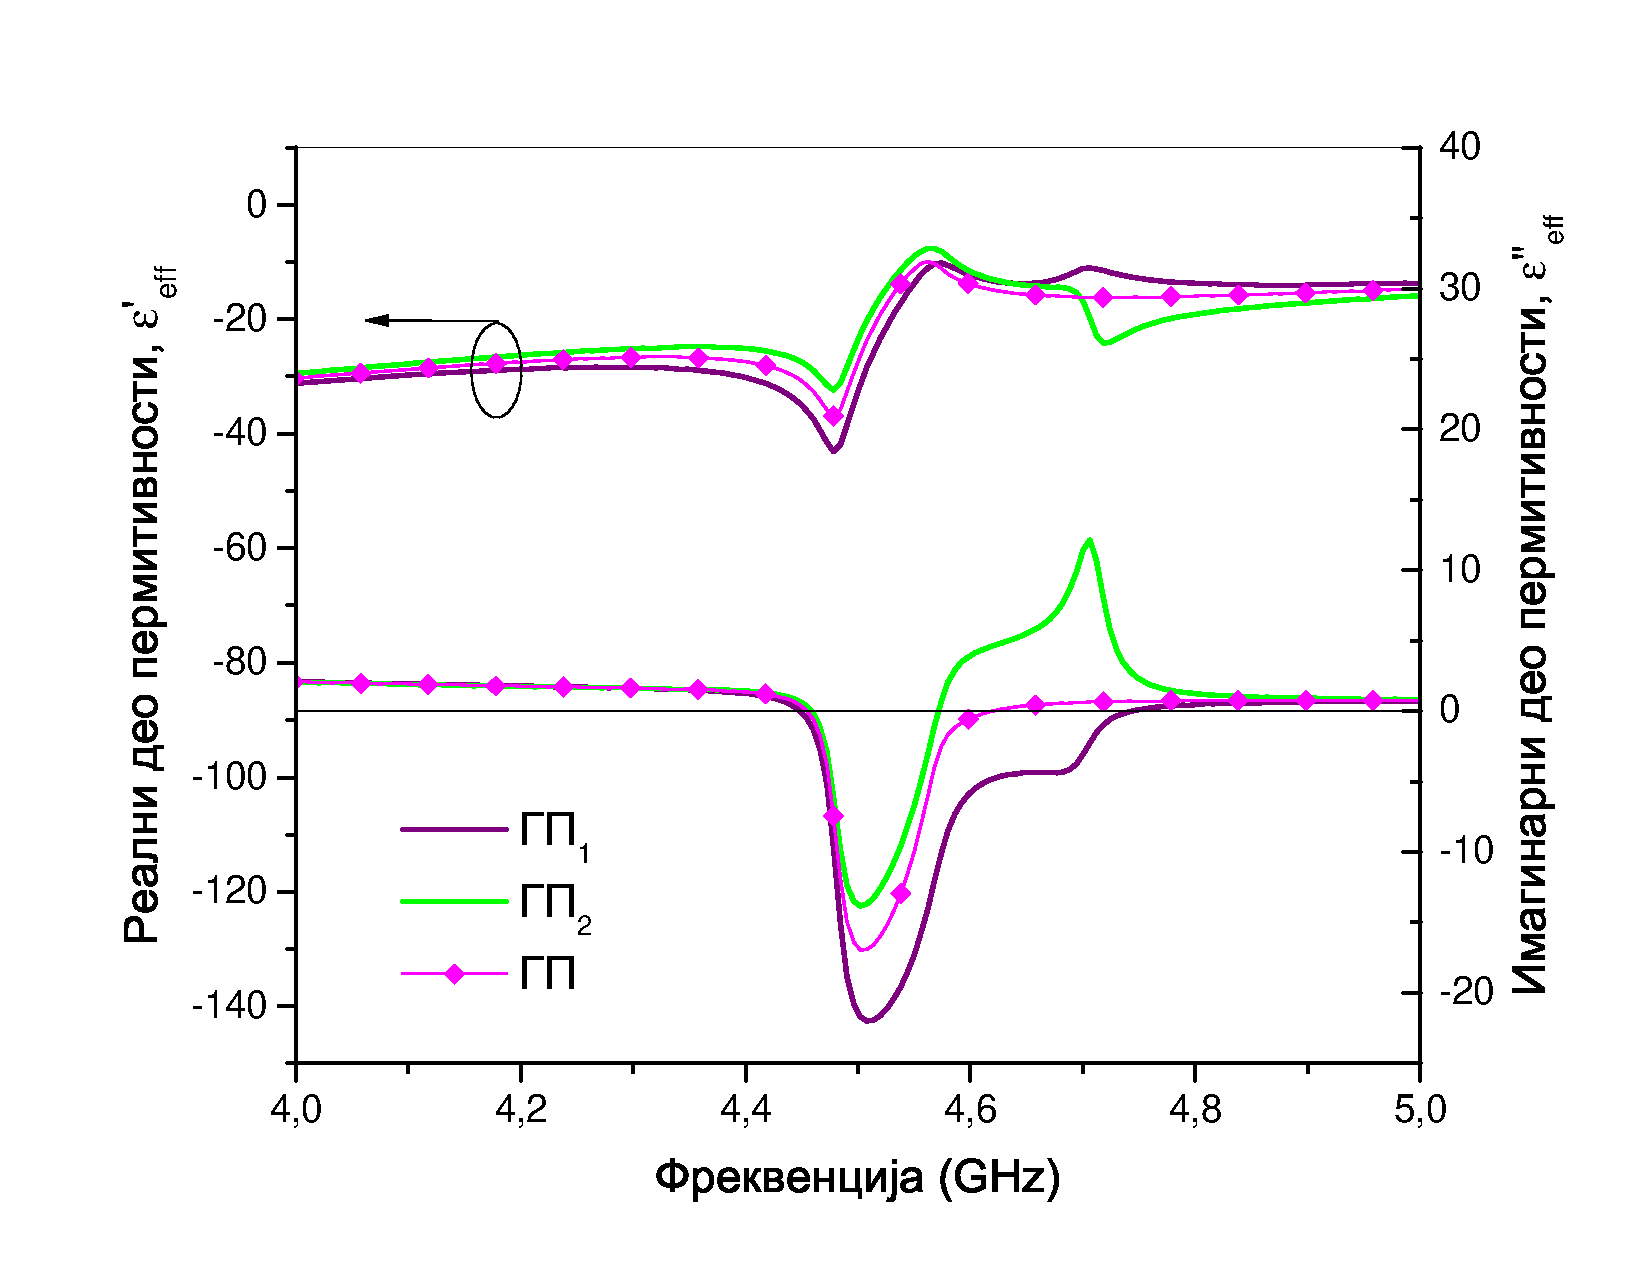
\includegraphics[width=0.6\textwidth]{slike/physcr/pod0/eps}
\label{ph:fig6a}}
\hfill
\subfloat[]{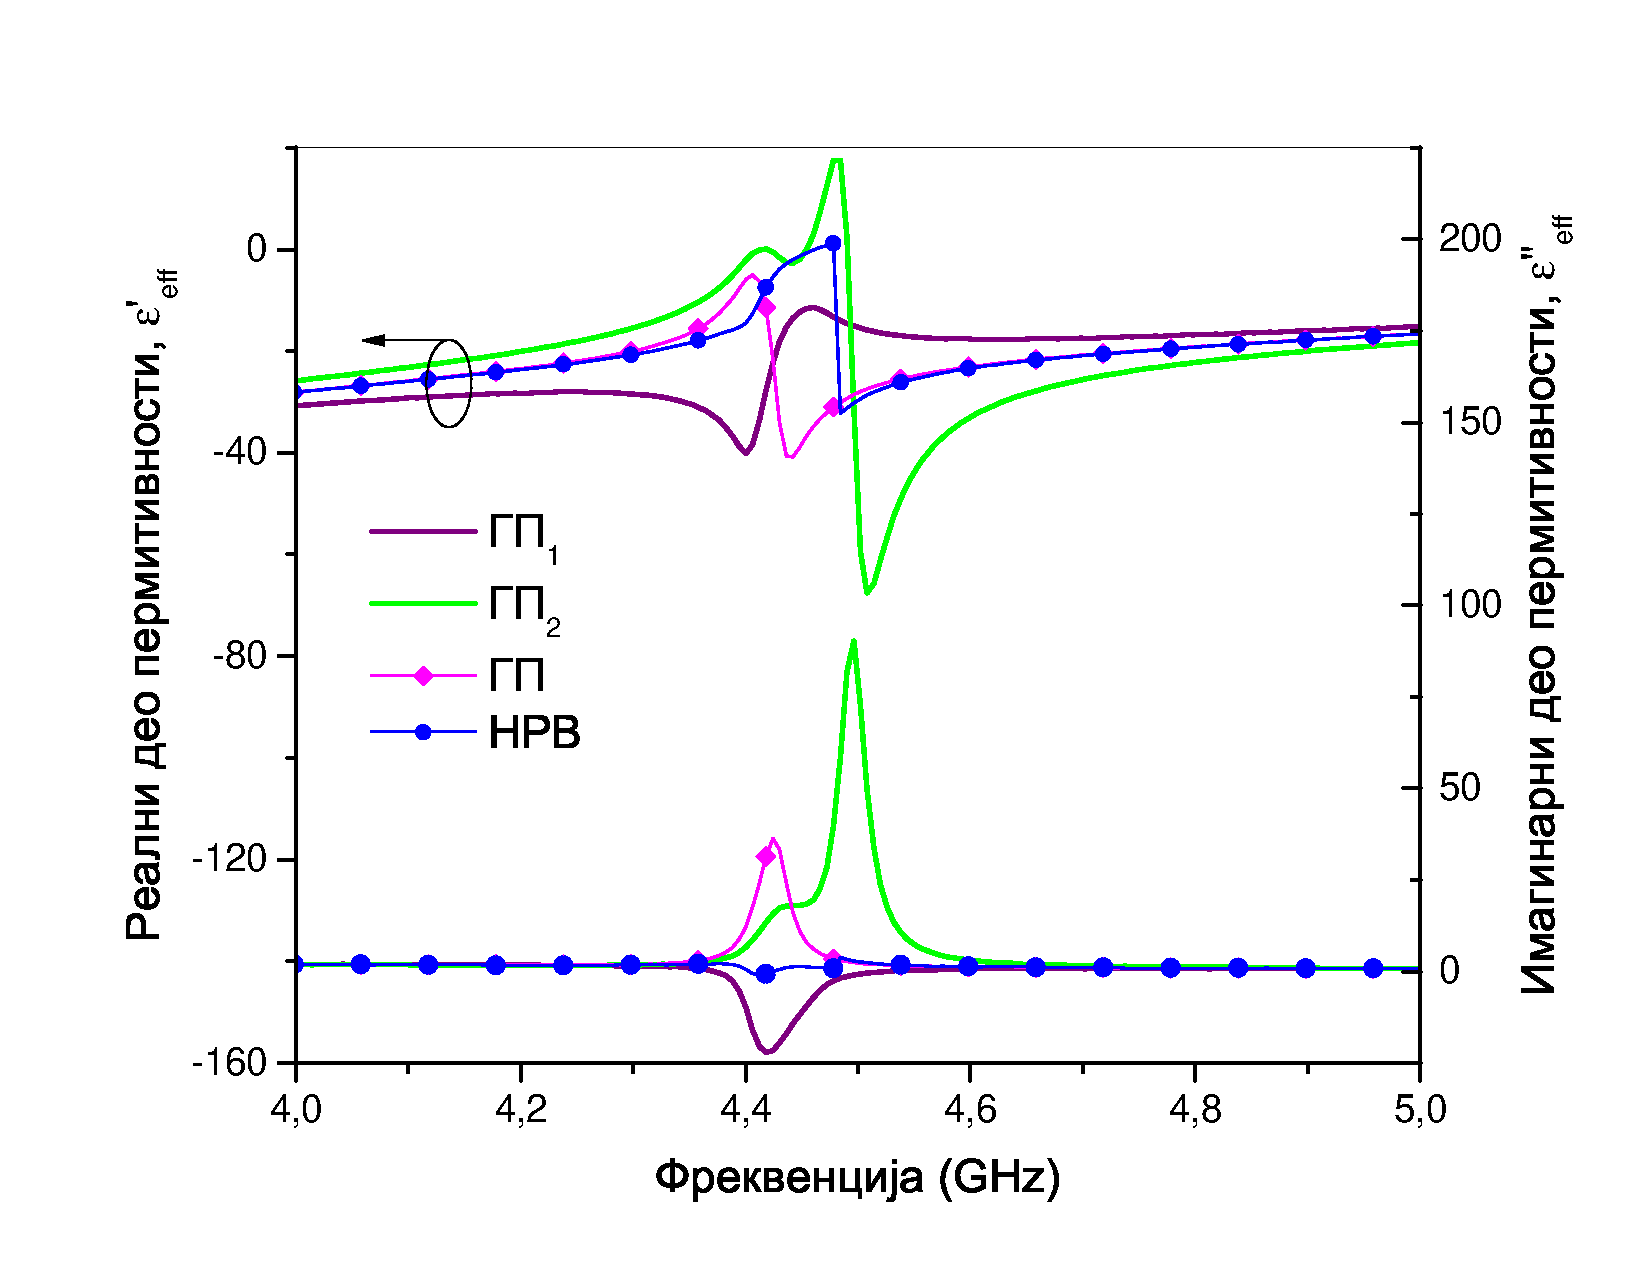
\includegraphics[width=0.6\textwidth]{slike/physcr/pod90/eps}
\label{ph:fig6b}}
\caption{Екстрахована ефективна пермитивност: \labelaslike}
\label{ph:fig6}
\end{figure} 

\begin{figure}[!t]
\centering
\subfloat[]{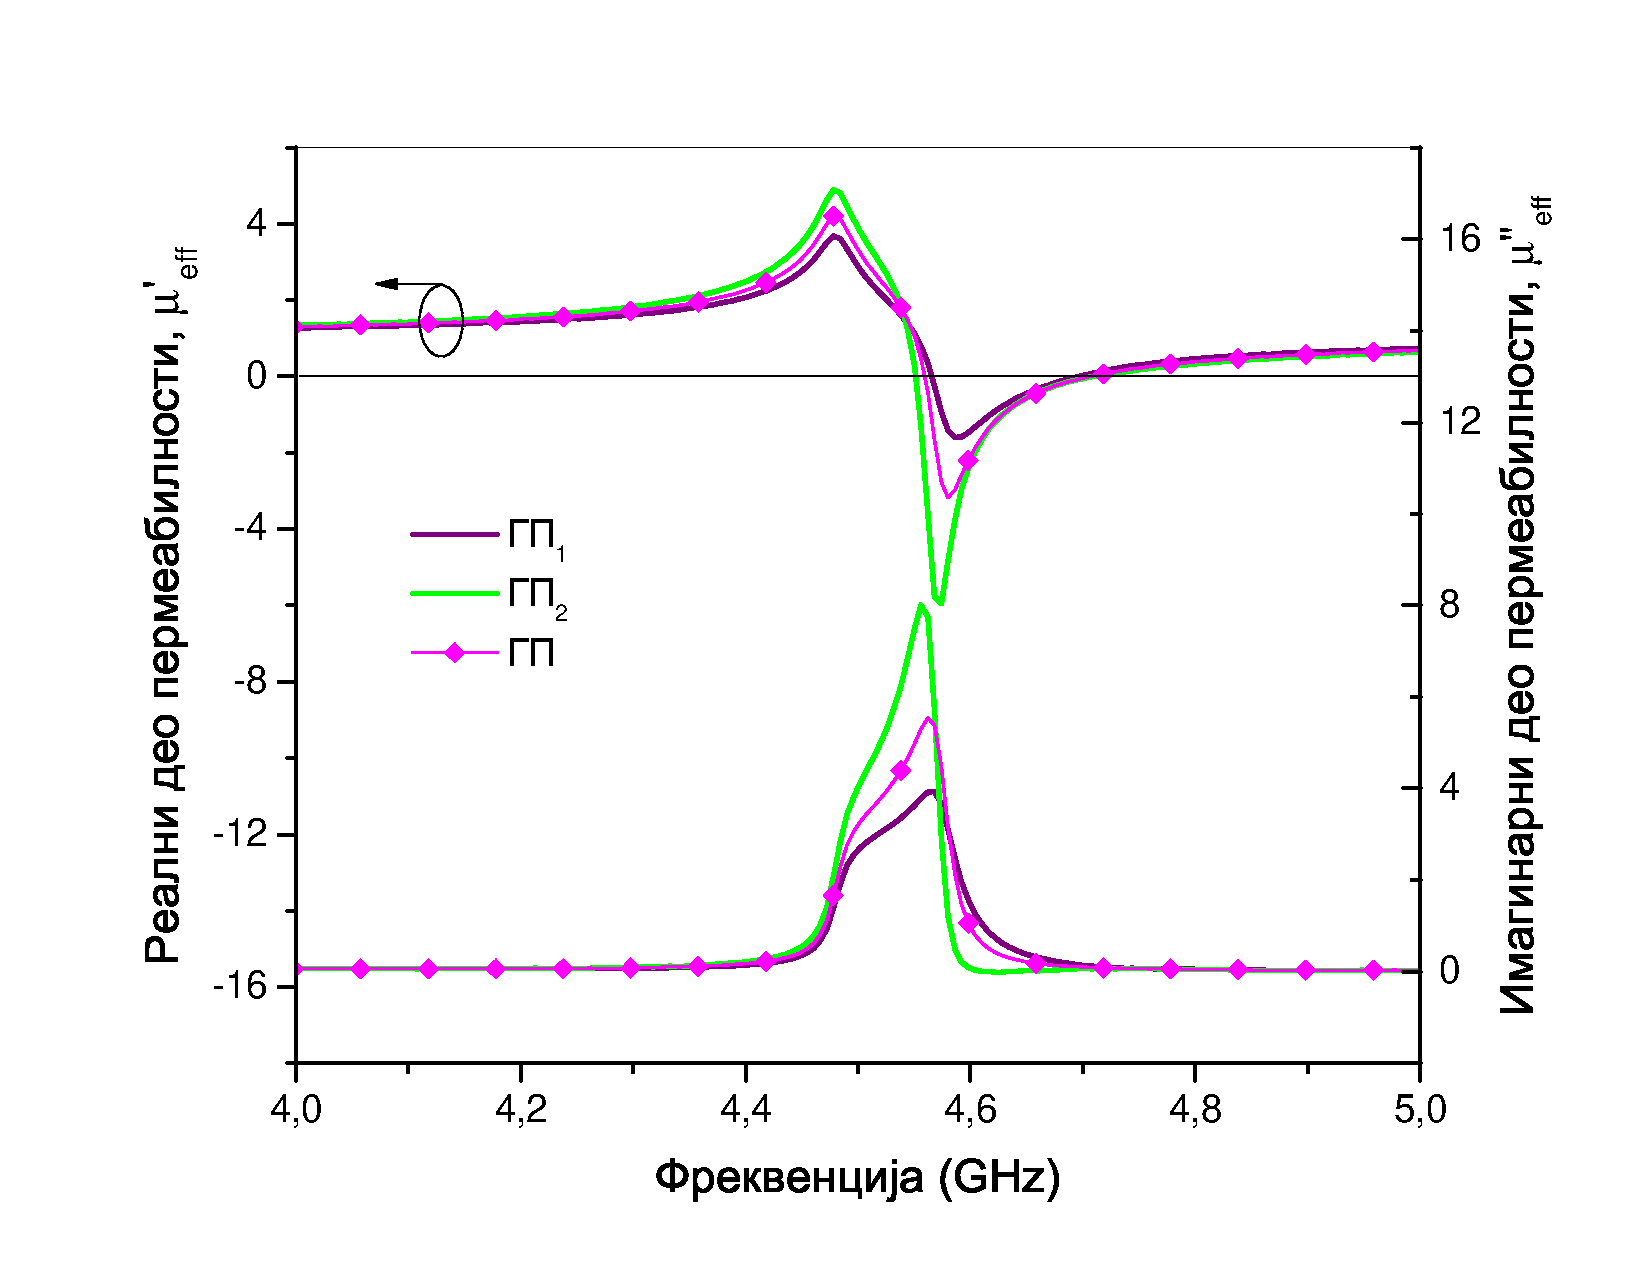
\includegraphics[width=0.6\textwidth]{slike/physcr/pod0/mi}
\label{ph:fig7a}}
\hfill
\subfloat[]{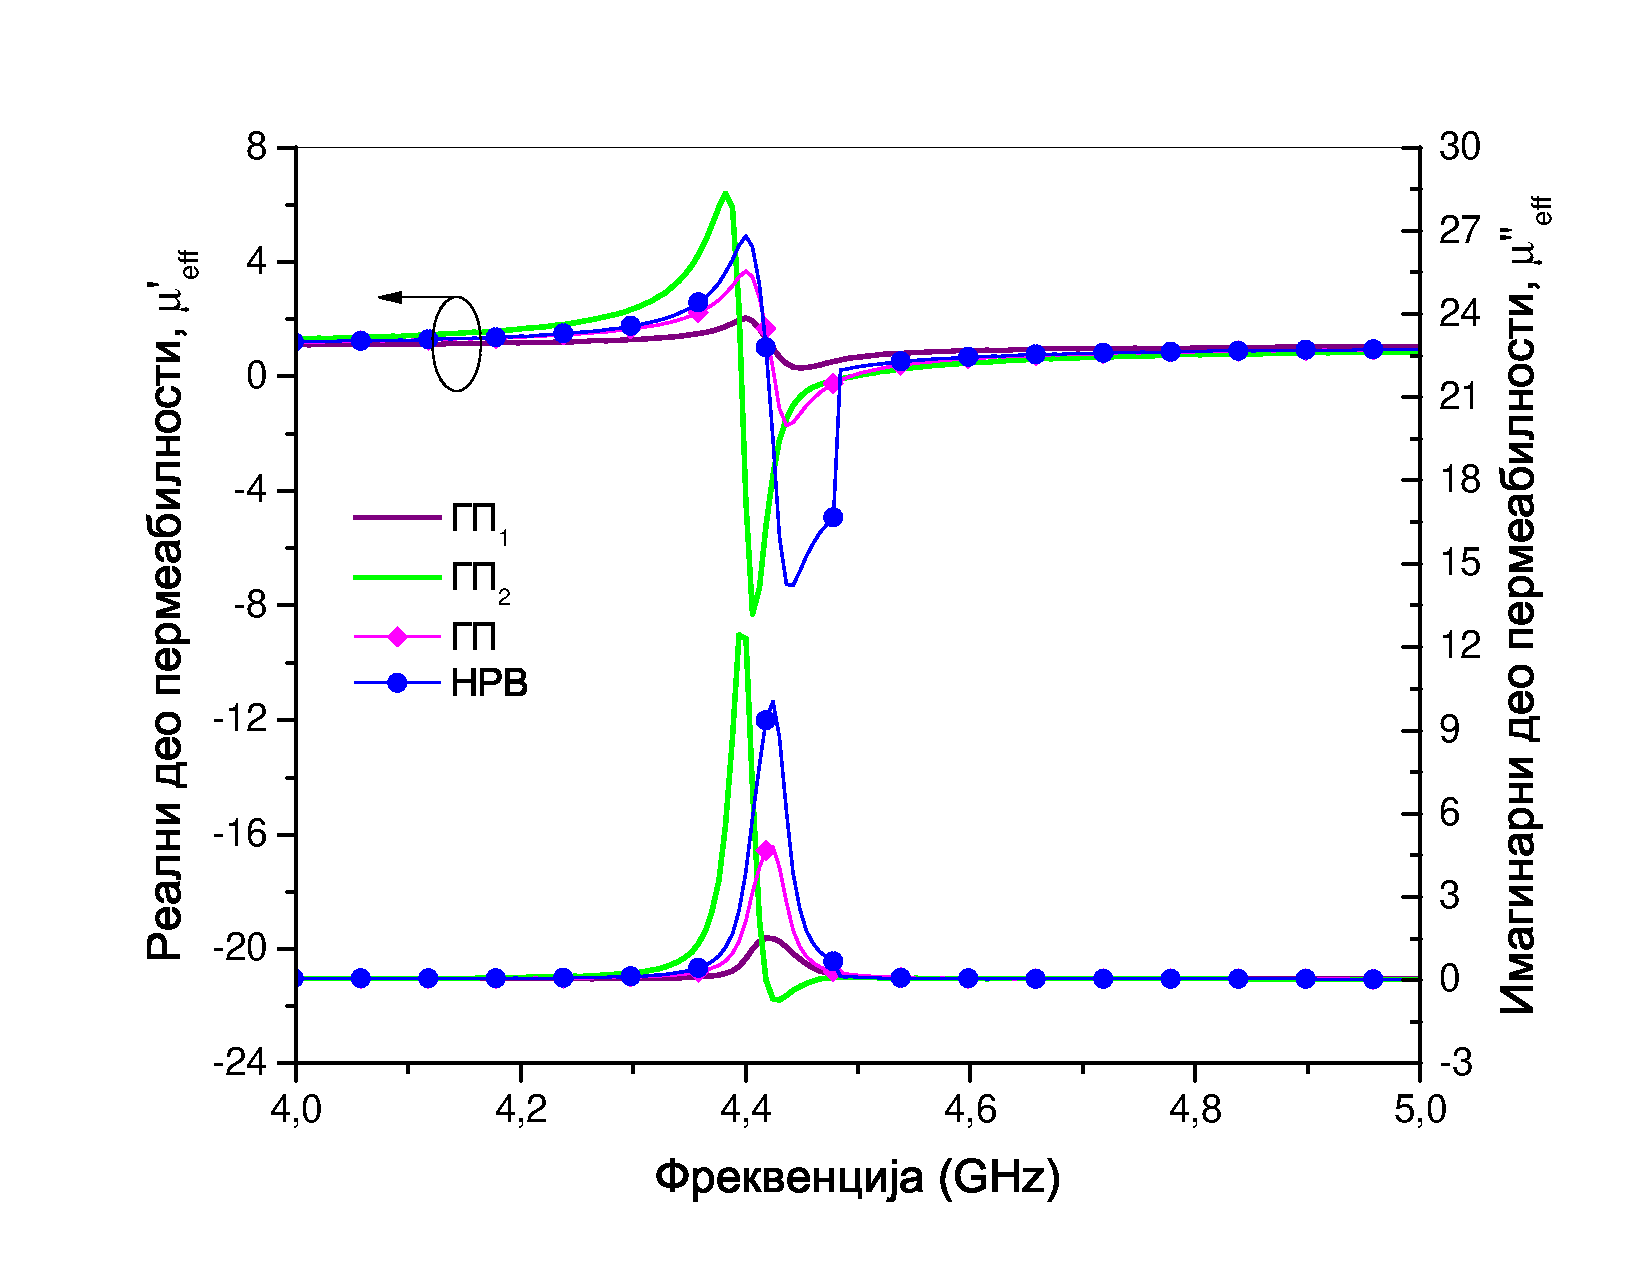
\includegraphics[width=0.6\textwidth]{slike/physcr/pod90/mi}
\label{ph:fig7b}}
\caption{Екстрахована ефективна пермеабилност: \labelaslike}
\label{ph:fig7}
\end{figure} 

\section{Валидација метода екстракције}\label{sekc4}
\subsection{Метод декомпозиције}
За проверу валидности предложене методе, може се користити независна симулација микрострип вода уроњеног у хомогени диелектрик са параметрима који одговарају екстрахованим вредностима, као што је приказано на сл.~\ref{slab}. Улазни микрострип водови су уроњени у ефективни диелектрик пермитивности $\varepsilon^{ML}_{eff}=3.15$. Приликом рачунања $Ѕ$-параметара [ефективног slaba], улазни водови се деембедују. Описана процедура се може непосредно применити за реконструкцију $Ѕ$-параметара добијених НРВ екстракцијом, која користи изотропни медијум описан са $\varepsilon$ и $\mu$, међутим [у тренутку писања рада] ауторима није било познато постојање програма за ЕМ анализу способног за рад са бианизотропним медијима.
\begin{figure}[!t]
\centering
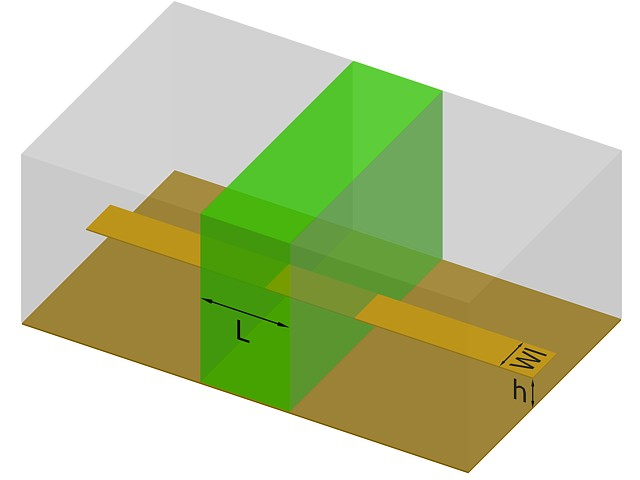
\includegraphics[width=0.6\columnwidth]{slike/slab.jpeg}
\caption{Слој ефективног медијума, који одговара асиметричној јединичној ћелији (зелени квадар) и улазни микрострип водови уроњени у ефективни диелектрик (светлосиви [квадри]). Релевантне димензије: $L=L_r+2L_m$, $h=h_1+h_2$, где су $L_r$, $L_m$, $h_1$, $h_2$ и $W_l$ дати на сл.~\ref{fig4}.}
\label{slab}
\end{figure}

Због тога, предложено је следеће [заобилазно] решење: симулирање два изотропна слоја, чији параметри одговарају онима добијеним $ГП_1$ и $ГП_2$ екстракцијама, на основу чега се добијају два сета $ABCD$ параметара, означених као $ABCD_{ГП1}$ and $ABCD_{ГП2}$, респективно. Сада, ако се пажљивије размотри релација (\ref{decomp}), примећује се да она представља дијагонализацију матрице, при чему $e^{\pm \gamma l}$ представљају сопствене вредности, а колоне матрице $Q$ сопствене векторе. Из (\ref{slicnost}) и (\ref{decomp}) следи да ће се матрице $ABCD_{ГП1,2}$, пошто оне подразумевају само једну вредност импедансе $Z_{c1,2}$, дијагонализовати у следећем облику:
\begin{equation}\label{decomp2}
ABCD_{ГП1,2} = Q_{1,2}\: \mathrm{diag}(e^{\gamma l},e^{-\gamma l})\: Q_{1,2}^{-1};
\end{equation}
where
\begin{equation}
Q_{1,2} = 
\begin{bmatrix}
1 & 1 \\
\frac{1}{Z_{c1,2}} & -\frac{1}{Z_{c1,2}}
\end{bmatrix}.
\end{equation}
Приметимо да су сопствене вредности $e^{\pm \gamma l}$ једнаке за све три матрице.

Из симулације слојева $ГП_{1,2}$ добијају се два сета $S$-параметара, који се могу конвертовати у $ABCD_{ГП1,2}$. Затим се врши дијагонализација ових матрица да би се добио облик (\ref{decomp2}). Оваква дијагонализација је лако доступна у програмским пакетима попут МАТЛАБ-а, и неопходно је само распоредити сопствене вредности и векторе на исти начин као у (\ref{decomp2}), што се може урадити на основу критеријума пасивности (\ref{pasivnost}). Сада је могуће добити матрицу $Q$ као
\begin{equation}
Q =
\begin{bmatrix}
Q_1(1,1) & Q_2(1,2) \\
Q_1(2,1) & Q_2(2,2)
\end{bmatrix},
\end{equation}
и, коначно, тражену $ABCD$ матрицу у складу са релацијом (\ref{decomp}).

\subsection{Јединичне ћелије са паралелним процепима}

$S$-параметри добијени описаним поступком, за јединичну ћелију са процепима паралелним и даље од вода (видети сл.~\ref{fig4b}), упоређени са оригиналним симулацијама, приказани су на сл.~\ref{val_pod180_mag}-\ref{val_pod180_ang}, за ГП и НРВ екстракције. НРВ метод (сл.~\ref{val_pod180nrw_mag} и \ref{val_pod180nrw_ang}) резултира са симетричним одзивом (због чега је само један коефицијент рефлексије, $S_{11}^{eff}=S_{22}^{eff}$, реконструисан), што очигледно не успева да тачно репродукује рефлексију у регионима са наглашеном асиметријом (осенченим на графику). Ово је највидљивије у фази, где се добијена вредност понања као средња вредност оригиналних фаза $S_{11}$ и $S_{22}$ (ово је очекивано због коришћене процедуре усредњавања).
\begin{figure}[!t]
\centering
\subfloat[]{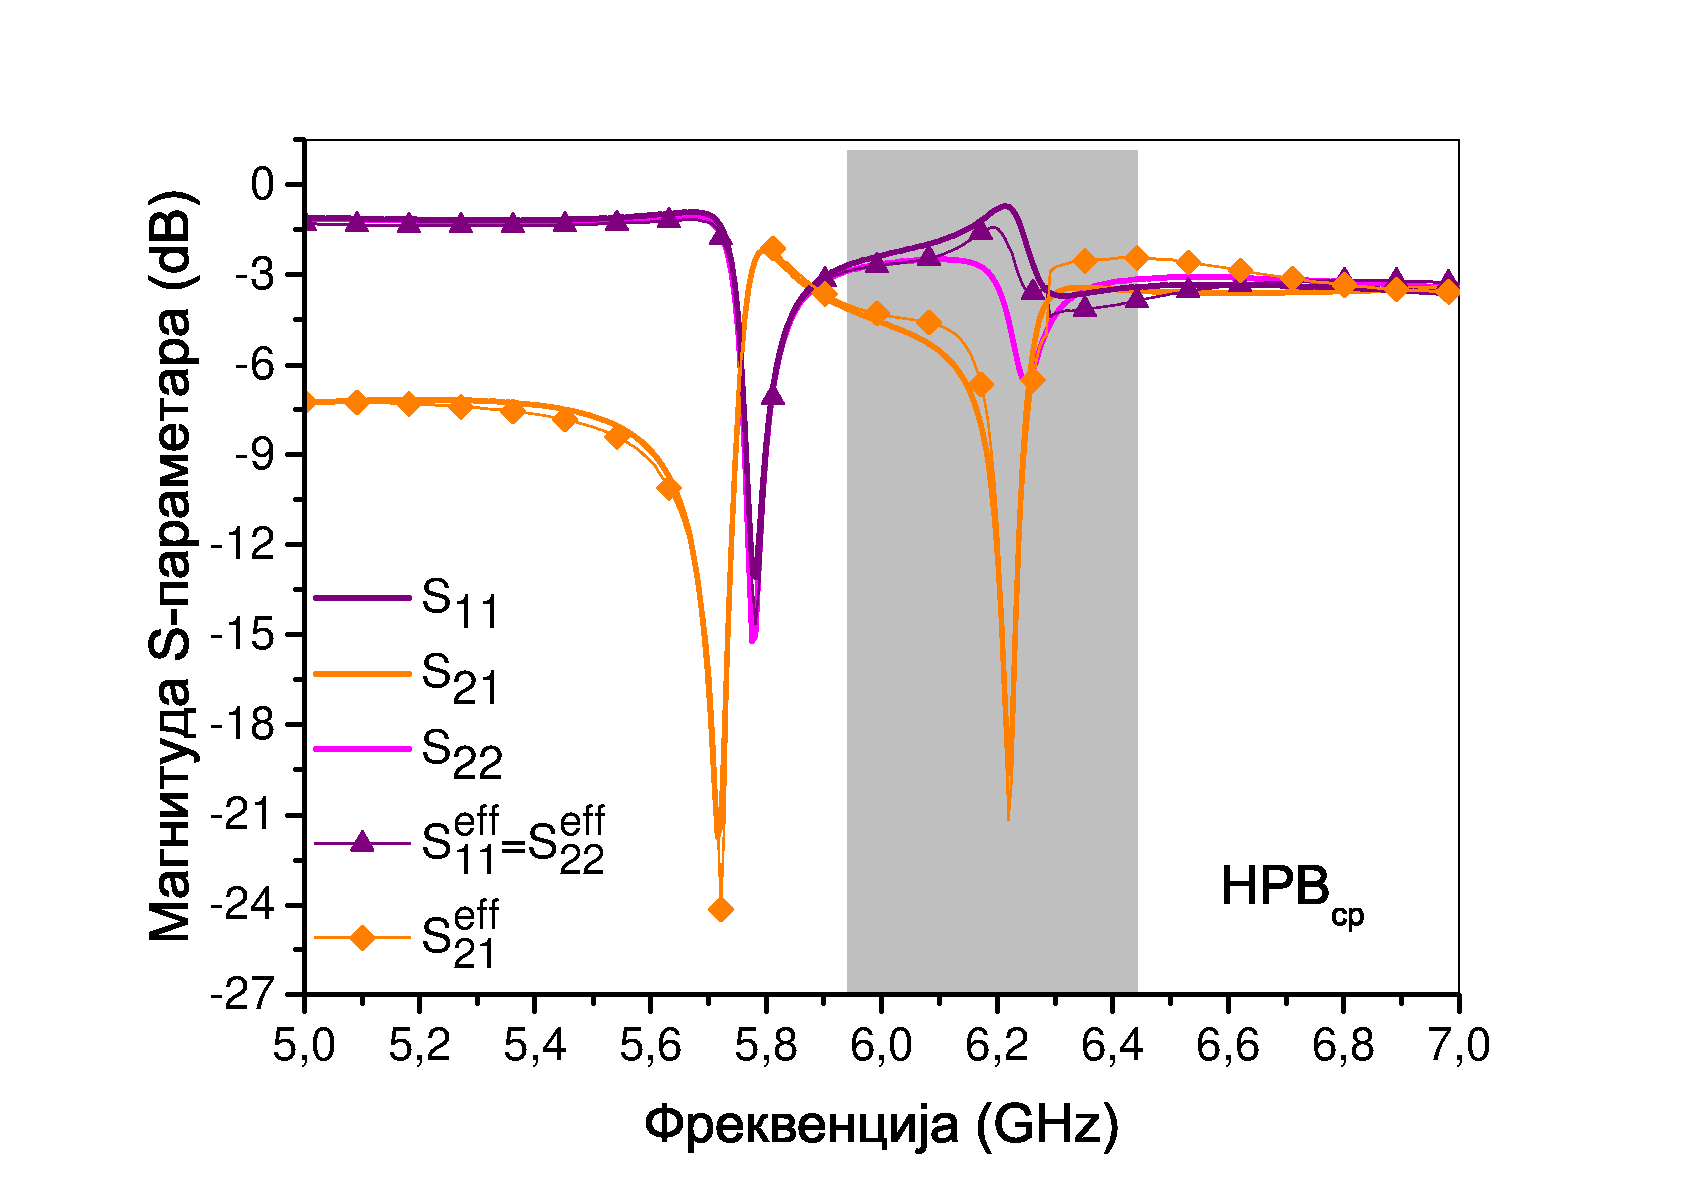
\includegraphics[scale=\SkalaC]{slike/val180nrw_mag.pdf}
\label{val_pod180nrw_mag}}
\subfloat[]{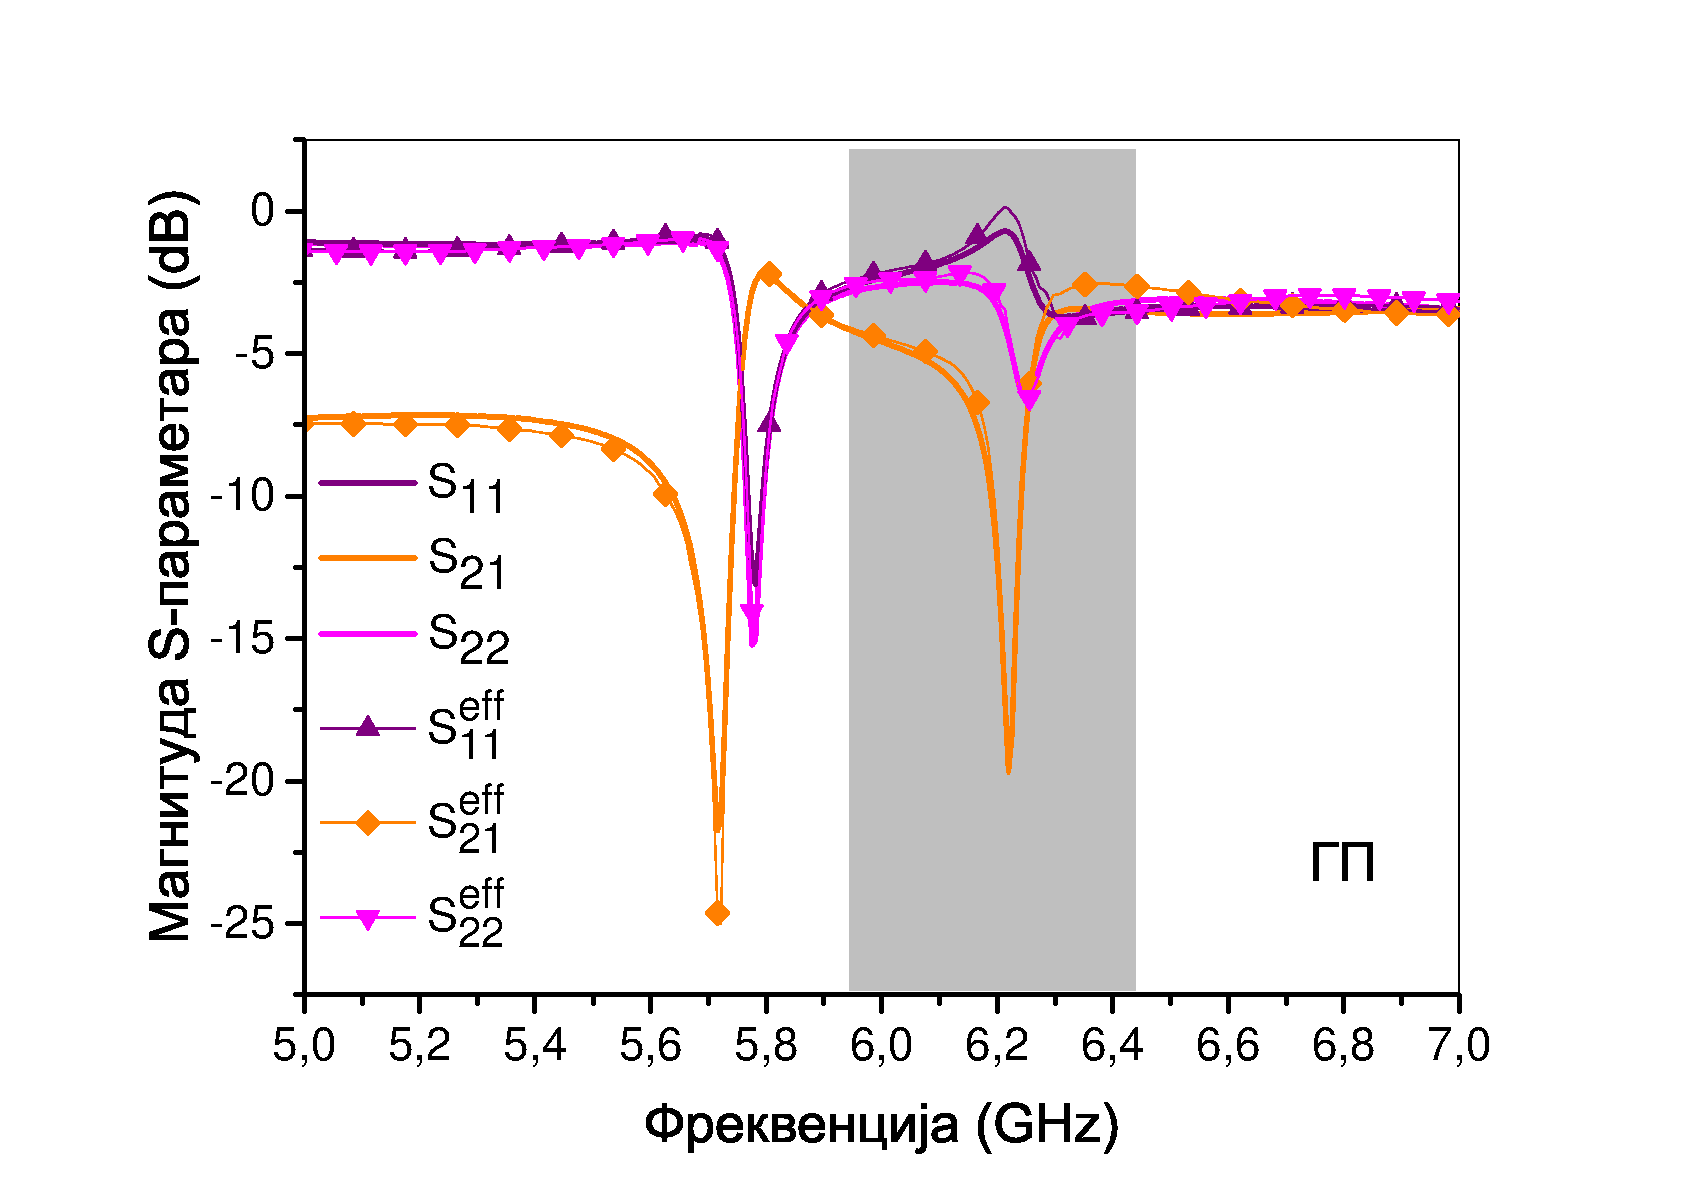
\includegraphics[scale=\SkalaC]{slike/val180ga_mag.pdf}
\label{val_pod180ga_mag}}
\caption{Магнитуда $S$-параметара симулираних и реконструисаних коришћењем ефективних параметара: (а) $НРВ_{СР}$ и (б) ГП екстракције. Осенчени делови означавају опсеге у којима се магнитуда $S_{11}$ и $S_{22}$ разликује.}
\label{val_pod180_mag}
\end{figure}
\begin{figure}[!t]
\centering
\subfloat[]{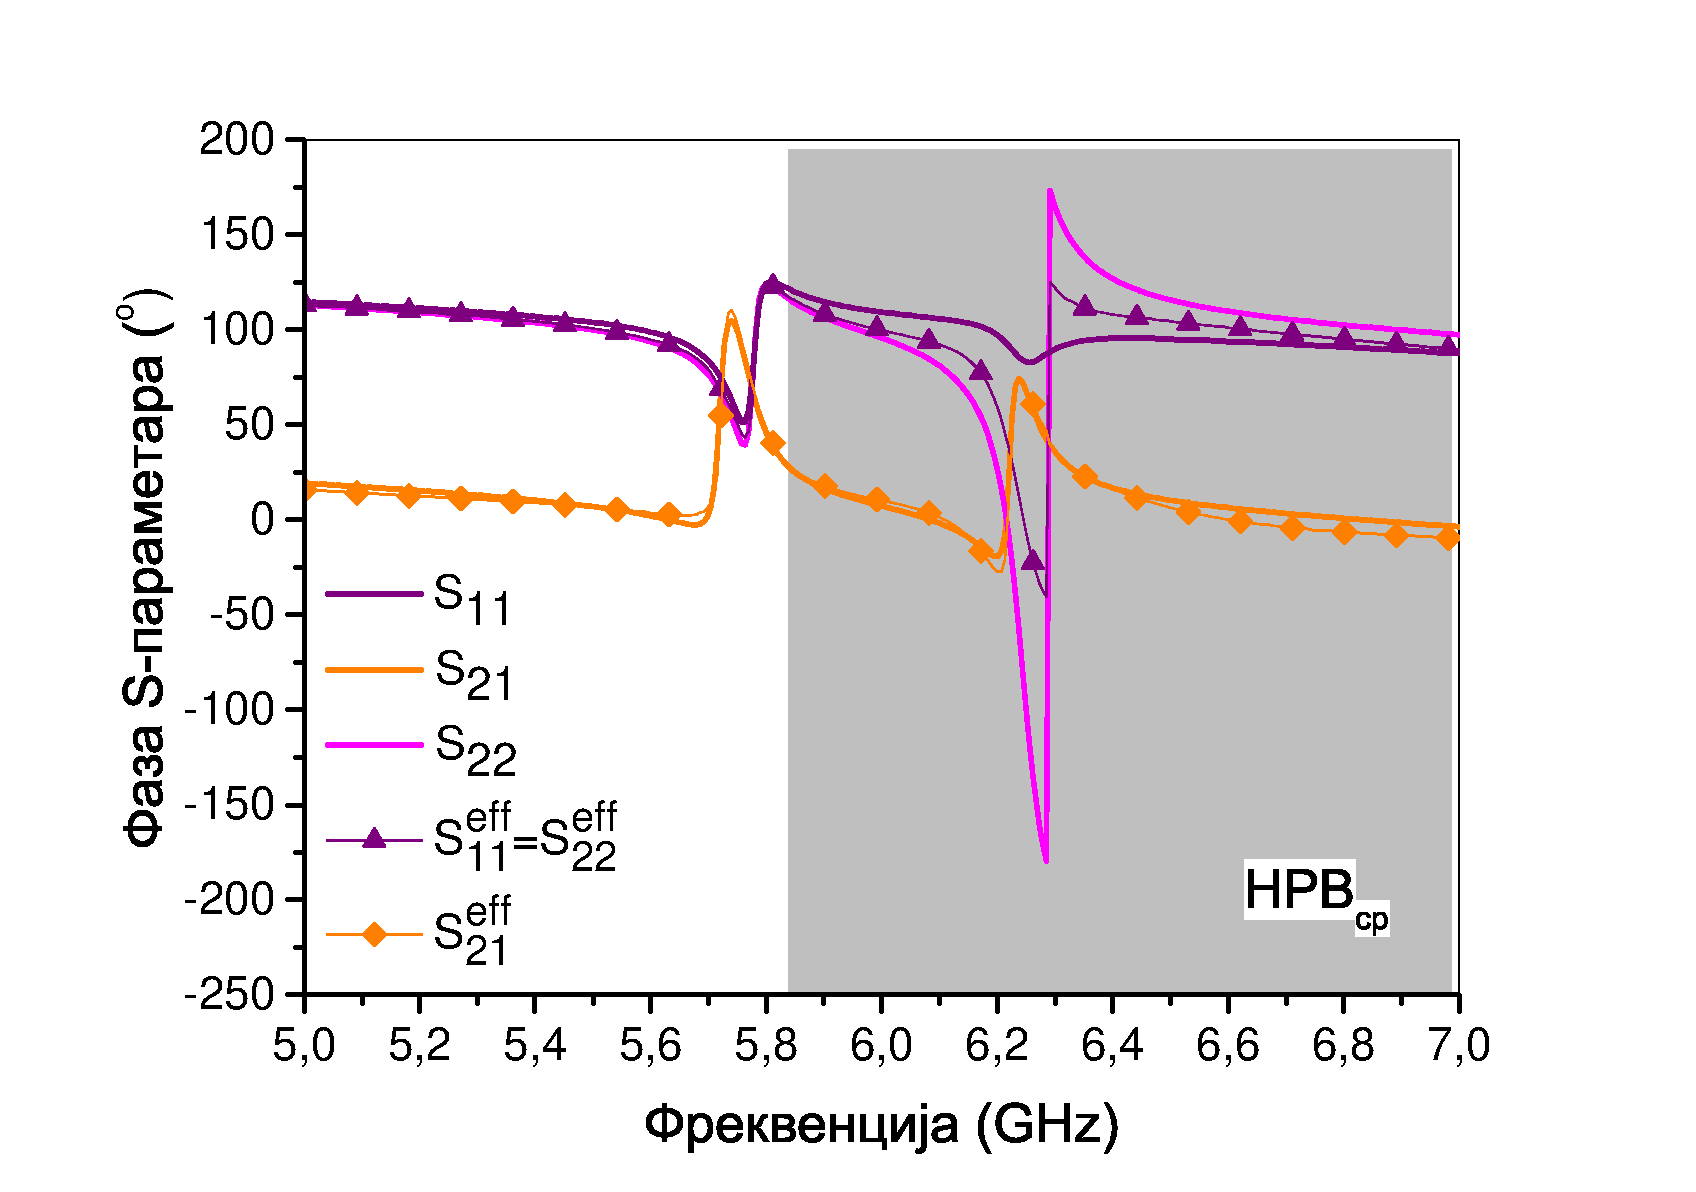
\includegraphics[scale=\SkalaC]{slike/val180nrw_ang.pdf}
\label{val_pod180nrw_ang}}
\subfloat[]{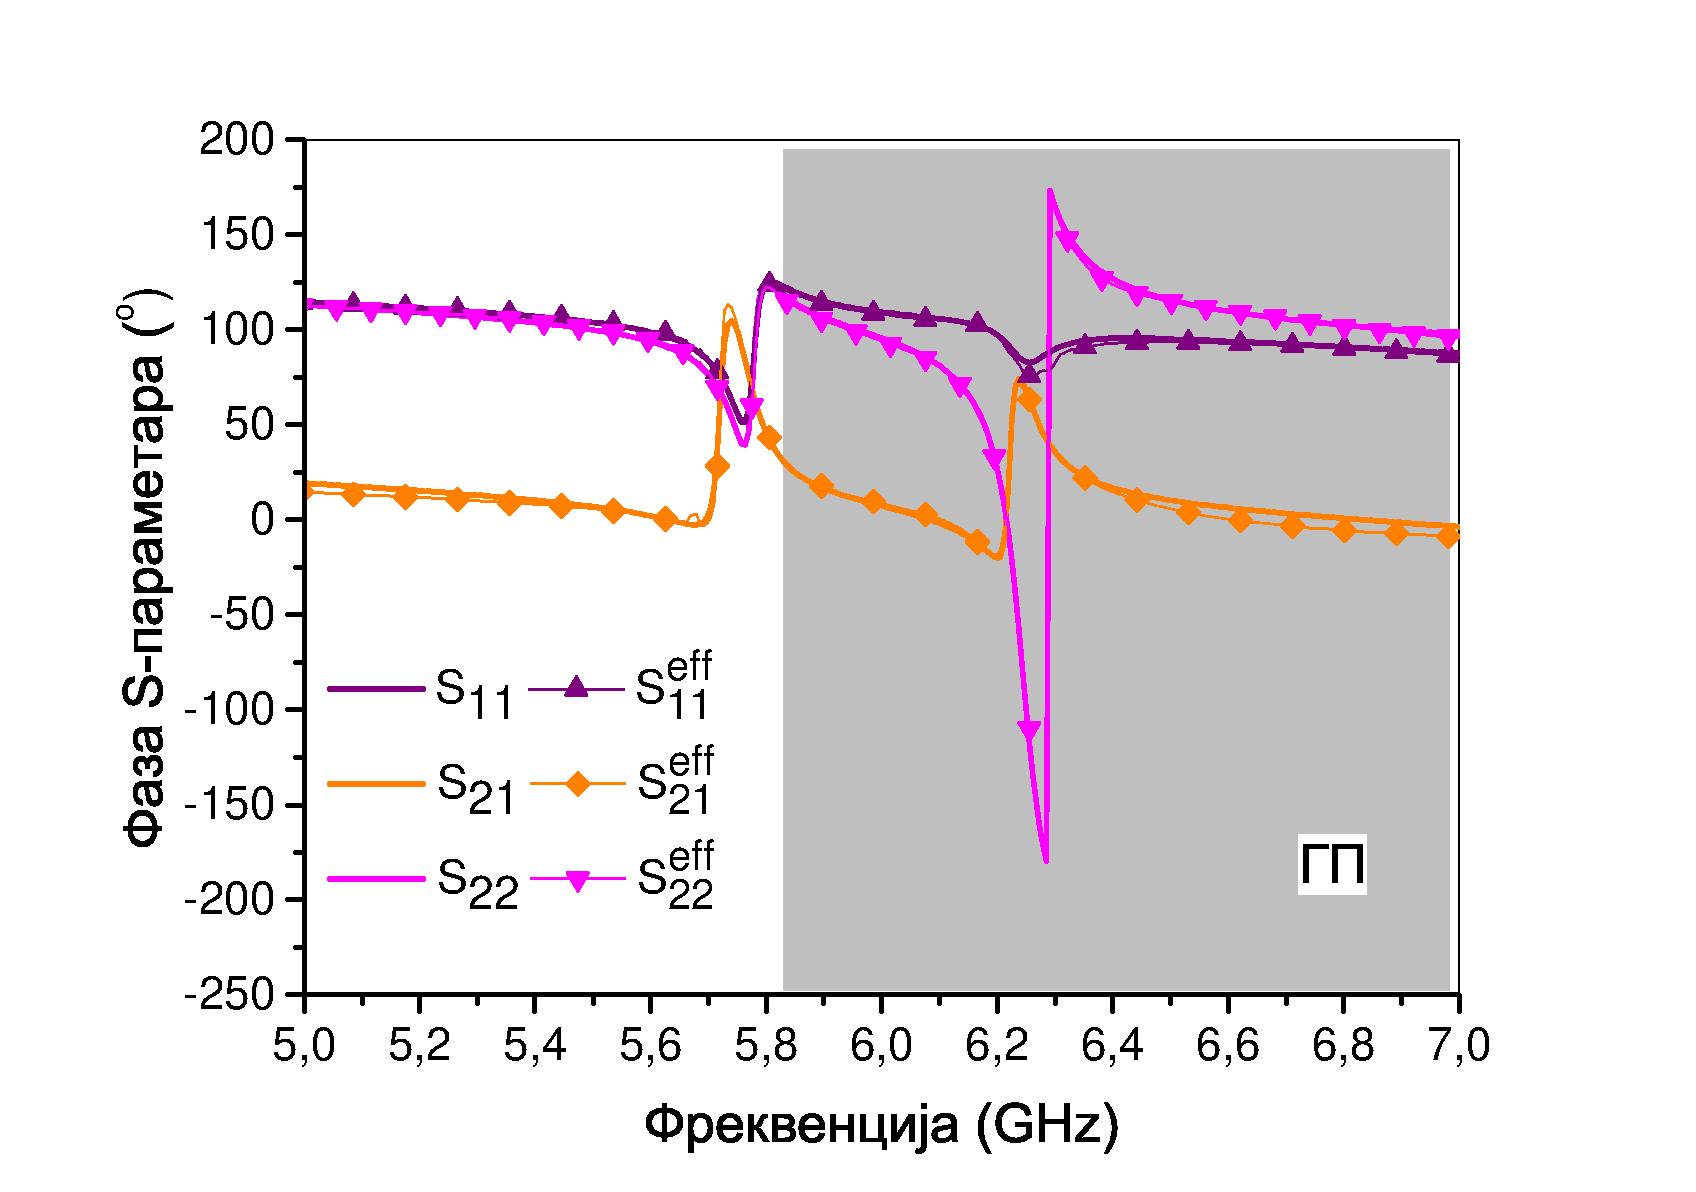
\includegraphics[scale=\SkalaC]{slike/val180ga_ang.pdf}
\label{val_pod180ga_ang}}
\caption{Фаза $S$-параметара симулираних и реконструисаних коришћењем ефективних параметара: (а) $НРВ_{СР}$ и (б) ГП екстракције.}
\label{val_pod180_ang}
\end{figure}

ГП метод, међутим, јасно разликује различите вредности коефицијената рефлексије, које су врло близу оригиналних вредности (видети сл.~\ref{val_pod180ga_mag} и \ref{val_pod180ga_ang}). Јасно се види да ефективни параметри добијени ГП методом омогућавају реконструкцију свих $S$-параметара, што није случај за $НРВ_{СР}$ методу, која омогућава реконструкцију само $S_{21}$, али не и $S_{11}$ и $S_{22}$ у опсезима где је присутна асиметрија. Ван тих опсега, ћелија има симетричан одзив и обе методе раде коректно.

\subsection{Јединичне ћелије са нормалним процепима}
Резултати за јединичну ћелију са нормалним процепом, са горњим процепом ближе воду (видети сл.~\ref{norm1}), упоређени са оригиналним симулацијама, су приказани на сл.~\ref{val_pod90_mag}-\ref{val_pod90_ang}, за $НРВ_{СР}$ и ГП екстракције. Поново, $НРВ_{СР}$ метод (видети сл.~\ref{val_pod90nrw_mag} и \ref{val_pod90nrw_ang}) репродукује само средњу вредност рефлексије, при чему је неслагање у овом случају још уочљивије, услед веће асиметричност ћелије. ГП метод поново блиско репродукује оба коефицијента рефлексије (видети сл.~\ref{val_pod90ga_mag} и \ref{val_pod90ga_ang}). Оба метода испољавају одређена неслагања, посебно у магнитуди $S_{21}$ изнад друге резонансе, која се могу приписати апроксимацији оригиналног вода, на коме се простире квази-ТЕМ мод, са водом у ефективном диелектрику, на коме се простире прави ТЕМ мод.
\begin{figure}[!t]
\centering
\subfloat[]{\includegraphics[scale=\SkalaC]{slike/val90nrw_mag.pdf}
\label{val_pod90nrw_mag}}
\subfloat[]{\includegraphics[scale=\SkalaC]{slike/val90ga_mag.pdf}
\label{val_pod90ga_mag}}
\caption{Магнитуда $S$-параметара симулираних и реконструисаних коришћењем ефективних параметара: (а) $НРВ_{СР}$ и (б) ГП екстракције. Осенчени делови означавају опсеге у којима се магнитуда $S_{11}$ и $S_{22}$ разликује.}
\label{val_pod90_mag}
\end{figure}
\begin{figure}[!t]
\centering
\subfloat[]{\includegraphics[scale=\SkalaC]{slike/val90nrw_ang.pdf}
\label{val_pod90nrw_ang}}
\subfloat[]{\includegraphics[scale=\SkalaC]{slike/val90ga_ang.pdf}
\label{val_pod90ga_ang}}
\caption{Фаза $S$-параметара симулираних и реконструисаних коришћењем ефективних параметара: (а) $НРВ_{СР}$ и (б) ГП екстракције.}
\label{val_pod90_ang}
\end{figure}

\subsection{Ивично спрегнути \emph{физскрипта}}
\begin{figure}[!t]
\centering
\subfloat[]{\includegraphics[scale=\SkalaA]{slike/physcr/pod0/valmag}}
%\hspace*{1cm}
\subfloat[]{\includegraphics[scale=\SkalaA]{slike/physcr/pod90/valmag}}
\caption{Magnitudes of $S$-parameters simulated and recovered using the effective bianisotropic parameters: \labelaslike}
\label{ph:fig8}
\end{figure} 

\begin{figure}[!t]
\centering
\subfloat[]{\includegraphics[scale=\SkalaA]{slike/physcr/pod0/valfaza}}
%\hspace*{1cm}
\subfloat[]{\includegraphics[scale=\SkalaA]{slike/physcr/pod90/valfaza}}
\caption{Phases of $S$-parameters simulated and recovered using the effective bianisotropic parameters: \labelaslike}
\label{ph:fig9}
\end{figure} 

\section{Закључак (ако то уопште иде у поглавље)}

У овом поглављу приказана је генералисана процедура за екстракцију ефективних параметара за метаматеријале на бази водова са асиметричном јединичном ћелијом. За описивање асиметрије, користи се еквивалентни бианизотропни медијум, који поред стандардних ефективних параметара поседује два додатна, $u$ и $\eta$, који су корисни као квантификација асиметричности. (спрега електричних и магнетних дипола, тј. крос-поларизабилност??)

Изведен је нови услов за негативни индекс преламања у бианизотропној средини. У поређењу са критеријумом за изотропне средине, услов је релаксиран у опсезима где су реални и имагинарни део параметра $u$ истог знака, а пооштрен тамо где су различитог знака.

Предложена генералисана процедура и НРВ метод са усредњавањем примењени су на нове дуал-бенд јединичне ћелије. Оне се састоје од БСЦ СРР-ова са процепима помереним у односу на центар одговарајуће ивице, постављеним један изнад другог.

Показано је да јединичне ћелије са паралелним процепима имају асиметрични одзив само око једне од резонанси, док су у остатку опсега симетричне. За разлику од тога, ћелије са нормалним процепима имају изражен асиметрични одзив око обе резонансе. Ефективна пермитивност и пермеабилност, добијене помоћу два метода, знатно се разликују, не само по апсолутним вредностима, већ некад имају и супротне знакове.

Показано је да НРВ процедура са усредњавањем даје тачан индекс преламања, али погрешне ефективне вредности пермитивности, пермеабилности и карактеристичне импедансе, и да се може користити само када је асиметрија веома слаба. Ово је потврђено поступком валидације, у коме је симулиран слој ефективног медијума са одговарајућим параметрима. Применом ГП метода, могуће је реконструисати вредности свих $Ѕ$-параметара, што није случај за параметре добијене НРВ поступком.
